%%                                    %%
%% Generated from MathBook XML source %%
%%    on 2014-10-05T14:37:40-05:00    %%
%%                                    %%
%%   http://mathbook.pugetsound.edu   %%
%%                                    %%
\documentclass[10pt,]{book}
%% Load geometry package to allow page margin adjustments
\usepackage{geometry}
\geometry{letterpaper,total={5.0in,9.0in}}
%% Custom Preamble Entries, early (use latex.preamble.early)
%% Inline math delimiters, \(, \), made robust with next package
\usepackage{fixltx2e}
%% Page Layout Adjustments (latex.geometry)
%% For unicode character support, use the "xelatex" executable
%% If never using xelatex, the next three lines can be removed
\usepackage{ifxetex}
\ifxetex\usepackage{xltxtra}\fi
%% Symbols, align environment, bracket-matrix
\usepackage{amsmath}
\usepackage{amssymb}
%% extpfeil package for certain extensible arrows,
%% as also provided by MathJax extension of the same name
\usepackage{extpfeil}
%% allow more columns to a matrix
%% can make this even bigger by overiding with  latex.preamble.late  processing option
\setcounter{MaxMatrixCols}{30}
%% XML, MathJax Conflict Macros
%% Two nonstandard macros that MathJax supports automatically
%% so we always define them in order to allow their use and
%% maintain source level compatibility
%% This avoids using two XML entities in source mathematics
\newcommand{\lt}{<}
\newcommand{\gt}{>}
%% Semantic Macros
%% To preserve meaning in a LaTeX file
%% Only defined here if required in this document
%% Used for inline definitions of terms
\newcommand{\terminology}[1]{\textbf{#1}}
%% Subdivision Numbering, Chapters, Sections, Subsections, etc
%% Subdivision numbers may be turned off at some level ("depth")
%% A section *always* has depth 1, contrary to us counting from the document root
%% The latex default is 3.  If a larger number is present here, then
%% removing this command may make some cross-references ambiguous
%% The precursor variable $numbering-maxlevel is checked for consistency in the common XSL file
\setcounter{secnumdepth}{1}
%% Environments with amsthm package
%% Theorem-like enviroments in "plain" style, with or without proof
\usepackage{amsthm}
\theoremstyle{plain}
%% Numbering for Theorems, Conjectures, Examples, Figures, etc
%% Controlled by  numbering.theorems.level  processing parameter
%% Always need a theorem environment to set base numbering scheme
%% even if document has no theorems (but has other environments)
\newtheorem{theorem}{Theorem}[chapter]
\renewcommand*{\proofname}{Proof}%% Only variants actually used in document appear here
%% Numbering: all theorem-like numbered consecutively
%% i.e. Corollary 4.3 follows Theorem 4.2
%% Equation Numbering
%% Controlled by  numbering.equations.level  processing parameter
\numberwithin{equation}{section}
%% Figures, Tables, Floats
%% The [H]ere option of the float package fixes floats in-place,
%% in deference to web usage, where floats are totally irrelevant
%% We redefine the figure and table environments, if used
%%   1) New mbxfigure and/or mbxtable environments are defined with float package
%%   2) Standard LaTeX environments redefined to use new environments
%%   3) Standard LaTeX environments redefined to step theorem counter
%%   4) Counter for new enviroments is set to the theorem counter before caption
%% You can remove all this figure/table setup, to restore standard LaTeX behavior
%% HOWEVER, numbering of figures/tables AND theorems/examples/remarks, etc
%% WILL ALL de-synchronize with the numbering in the HTML version
%% You can remove the [H] argument of the \newfloat command, to allow flotation and 
%% preserve numbering, BUT the numbering may then appear "out-of-order"
\usepackage{float}
\newfloat{mbxfigure}{H}{lof}[chapter]
\floatname{mbxfigure}{Figure}
\renewenvironment{figure}%
{\begin{mbxfigure}\setcounter{mbxfigure}{\value{theorem}}\stepcounter{theorem}}%
{\end{mbxfigure}}
%% Raster graphics inclusion, wrapped figures in paragraphs
\usepackage{graphicx}
%% Colors for Sage boxes and author tools (red hilites)
\usepackage[usenames,dvipsnames,svgnames,table]{xcolor}
%% Program listing support, for Sage code or otherwise
\usepackage{listings}
%% We define \listingsfont to provide Bitstream Vera Mono font
%% for program listings, under both pdflate and xelatex
%% If you remove this, define \listingsfont to be \ttfamily perhaps
\ifxetex
\usepackage{fontspec}\newfontface\listingsfont[Path]{fvmr8a.pfb}
\else
\edef\oldtt{\ttdefault}\usepackage[scaled]{beramono}\usepackage[T1]{fontenc}
\renewcommand*\ttdefault{\oldtt}\newcommand{\listingsfont}{\fontfamily{fvm}\selectfont}
\fi
%% End of program listing font definition
%% Sage's blue is 50%, we go way lighter (blue!05 would work)
\definecolor{sageblue}{rgb}{0.95,0.95,1}
%% Sage input, listings package: Python syntax, boxed, colored, line breaking
\lstdefinestyle{sageinput}{language=Python,breaklines=true,breakatwhitespace=true,basicstyle=\footnotesize\listingsfont,columns=fixed,frame=single,backgroundcolor=\color{sageblue},xleftmargin=4ex,xrightmargin=4ex}
%% Sage output, similar, but not boxed, not colored
\lstdefinestyle{sageoutput}{language=Python,breaklines=true,breakatwhitespace=true,basicstyle=\footnotesize\listingsfont,columns=fixed,xleftmargin=8ex,xrightmargin=4ex}
%% hyperref driver does not need to be specified
\usepackage{hyperref}
%% latex.print parameter set to 'yes', all hyperlinks black
\hypersetup{hidelinks}
\hypersetup{pdftitle={Math 2500: Linear Algebra}}
%% If you manually remove hyperref, leave in this next command
\providecommand\phantomsection{}
%% Custom Preamble Entries, late (use latex.preamble.late)
\newtheorem{task}{Task}[chapter]

%% Convenience macros
\newcommand{\augmatrix}[2]{\left(\begin{array}{@{}#1 |c@{}} #2 \end{array}\right)}
%% Title page information for book
\title{Math 2500: Linear Algebra}
\author{}
\date{}
\begin{document}
\frontmatter
%% half-title
\thispagestyle{empty}
\vspace*{\stretch{1}}
\begin{center}
{\Huge Math 2500: Linear Algebra}
\end{center}\par
\vspace*{\stretch{2}}
\clearpage
\thispagestyle{empty}
\clearpage
\maketitle
\clearpage
\thispagestyle{empty}
\vspace*{\stretch{2}}
\vspace*{\stretch{1}}
\clearpage
\setcounter{tocdepth}{1}
\renewcommand*\contentsname{Contents}
\tableofcontents
\chapter{Preface}
This is a set of class notes designed to guide an inquiry-based course
      on linear algebra. This is not a complete resource! Rather, this text is
      meant to accompany the book Introduction to Linear Algebra by
      Gilbert Strang. Industrious students might also use it for a self-study
      course.
    %
\par
An important feature of this text is the integration of the Sage
      Mathematical Software System. Students in this course will learn to use
      Sage to perform long tedious computations (which linear algebra has in
      spades) and create visualizations.
    %
I thank the Sage community, in particular William Stein, for creating
      such a wonderful tool and making it open-source.
    %
\par
I also thank Rob Beezer for creating the MathBook project which makes
      this particular book project available on the web.
    %
\mainmatter
\typeout{************************************************}
\typeout{Chapter 1 Vectors, the Dot Product, and Matrices}
\typeout{************************************************}
\chapter[Vectors, the Dot Product, and Matrices]{Vectors, the Dot Product, and Matrices}\label{chapter-basic-objects}

      This first chapter introduces the basic objects of linear algebra.
      You will meet vectors, the dot product, and matrices.
    %
\par

      Vectors are a generalization of the concept of number. Where real numbers
      can help us model the geometry of points on a line, vectors will allow us to
      model the geometry of a plane, or (three-dimensional) space, or even "spaces"
      with higher dimensions. We begin by learning about the algebra of vectors,
      and making connections to the geometry.
    %
\par

      The dot product is a funny kind of multiplication. It plays an important
      role in mathematics because it captures all of the basics of measurement.
      We shall learn how to use the dot product to measure lengths and angles. By
      its definition, the dot product is connected with the concept of a linear
      equation, so it will make frequent appearances in our work.
    %
\par

      Matrices are another way to generalize the concept of number. (In fact, they
      generalize the concept of vector.) We start here by learning about the
      algebra of matrices. The whole rest of this course will focus on matrices,
      their uses, and their properties.
    %
\par

      A running theme for this course is the use of the Sage mathematical software
      system. In order to get started, the fourth section of this course is
      dedicated to getting started with Sage using the SageMathCloud (SMC). You will
      make an account and run through an introductory workshop with SMC.
      Also, throughout this workbook you will find little embedded pieces of Sage
      code. These are implemented using the Sage SingleCell server. Most of these
      Sage cells are mutable. You can change the content in them and re-evaluate
      your new Sage code. I encourage you to play with these---it is a good way to
      learn the basics of Sage.
    %
\par

      The fifth and final section of the chapter is a short assignment designed to
      consolidate learning. You will get a chance to practice your skills and to
      think more deeply about the concepts you have learned.
    %
\typeout{************************************************}
\typeout{Section 1.1 Vectors}
\typeout{************************************************}
\section[Vectors]{Vectors}\label{vectors}
\typeout{************************************************}
\typeout{Subsection  The Assignment}
\typeout{************************************************}
\subsection[The Assignment]{The Assignment}\label{subsection-1}
\begin{itemize}
\item{}Read section 1.1 of \emph{Strang} (pages 1-7).\item{}Read the following and complete the exercises below.\end{itemize}
\typeout{************************************************}
\typeout{Subsection  Learning Objectives}
\typeout{************************************************}
\subsection[Learning Objectives]{Learning Objectives}\label{subsection-2}
Before class, a student should be able to:
      \begin{itemize}
\item{}Add vectors.\item{}Multiply a vector by a scalar.\item{}Compute linear combinations.\item{}Draw pictures which correspond to the above operations.\end{itemize}

      At some point, a student should be able to:
      \begin{itemize}
\item{}Solve linear combination equations involving unknown coefficients.\item{}Solve linear combination equations involving unknown vectors.\end{itemize}

    %
\typeout{************************************************}
\typeout{Subsection  Some Discussion}
\typeout{************************************************}
\subsection[Some Discussion]{Some Discussion}\label{subsection-3}
Algebraically, a \terminology{vector} is a stack of numbers in a set of
     parentheses or brackets, like this\begin{align*}
\begin{pmatrix} 2 \\ 7 \\ 9 \end{pmatrix}, \text{ or }
          \begin{bmatrix}2 \\ 7 \\ 9 \end{bmatrix}, \text{ or }
          \begin{pmatrix} 2 & 7 & 9 \end{pmatrix}.
\end{align*}
     The individual numbers are called the \terminology{components} or \terminology{entries}
     or \terminology{coordinates} of the vector. For example, \(7\) is the second
     component of the vectors above.%
\par
The first two vectors above are called \terminology{column} vectors
        because they are stacked vertically. The third is called a \terminology{row} vector because it is arranged horizontally. For this class, we will always use column vectors, but to save space, we might sometimes write them as row vectors. It is up to you to make the switch. (We will see later how this matters!)%
\par
Vectors can take lots of different sizes. The vectors above are all \(3\)-vectors. Here is a \(2\)-vector: \[\begin{pmatrix} 71 \\ -12 \end{pmatrix}.\] Here is a \(4\)-vector: \[\begin{pmatrix} \pi \\ 0 \\ -\pi \\ 1\end{pmatrix}.\]%
\par
The main value in using vectors lies in their standard interpretations. Let's focus on \(3\)-vectors for now. The vector \(\left(\begin{smallmatrix} a \\ b \\ c\end{smallmatrix}\right)\) can represent \begin{itemize}
\item{}A point in space described in the standard three-dimensional rectangular coordinate system with \(x\) coordinate equal to \(a\), \(y\)-coordinate equal to \(b\) and \(z\) coordinate equal to \(c\).%
\item{}An arrow in space which points from the origin \((0,0,0)\) to the point \((a,b,c)\).%
\item{}An arrow in space which points from some point \((x,y,z)\) to the point \((x+a,y+b,z+c)\).%
\end{itemize}

        %
\typeout{************************************************}
\typeout{Subsubsection  Operations on Vectors}
\typeout{************************************************}
\subsubsection[Operations on Vectors]{Operations on Vectors}\label{subsubsection-1}
There are two operations on vectors which are of utmost importance for linear algebra. (In fact, if your problem has these operations in it, there is a chance you are doing linear algebra already.)%
\typeout{************************************************}
\typeout{Paragraph  Scalar Multiplication}
\typeout{************************************************}
\paragraph[Scalar Multiplication]{Scalar Multiplication}\label{paragraph-1}
Given a number \(\lambda \in \mathbb{R}\) and a vector \(v = \left(\begin{smallmatrix} a \\ b \\ c \end{smallmatrix}\right)\), we form the new vector \[\lambda v = \left(\begin{smallmatrix} \lambda a \\ \lambda b \\ \lambda c \end{smallmatrix}\right).\]%
\typeout{************************************************}
\typeout{Paragraph  Addition}
\typeout{************************************************}
\paragraph[Addition]{Addition}\label{paragraph-2}
Given a vector \(v = \left(\begin{smallmatrix} a \\ b \\ c \end{smallmatrix}\right)\) and a vector \(w = \left(\begin{smallmatrix} d \\ e \\ f \end{smallmatrix}\right)\) of the same size, we form their \terminology{sum} \[ v+w = \left(\begin{smallmatrix} a+d \\ b+e \\ c+f \end{smallmatrix}\right) \]%
\typeout{************************************************}
\typeout{Paragraph }
\typeout{************************************************}
\paragraph[]{}\label{paragraph-3}
These operations have ``obvious'' generalizations to vectors of different sizes. Because things go entry-by-entry, these are often called \terminology{coordinate-wise} operations.%
\par
Combining these two operations gives us the notion of a \emph{linear combination}. If \(\lambda\) and \(\mu\) are numbers and \(v\) and \(w\) are vectors of a common size, then the vector \[\lambda v + \mu w \] is a linear combination of \(v\) and \(w\).%
\typeout{************************************************}
\typeout{Subsection  Sage Instructions}
\typeout{************************************************}
\subsection[Sage Instructions]{Sage Instructions}\label{subsection-4}
\typeout{************************************************}
\typeout{Paragraph  Basic Constructions}
\typeout{************************************************}
\paragraph[Basic Constructions]{Basic Constructions}\label{paragraph-4}
A vector in Sage is constructed by applying the \verb?vector? command to a list. Lists are entered in square brackets with entries separated by commas, so the typical way to create a vector looks like this:%
\begin{lstlisting}[style=sageinput]
u = vector([1,1,2])
\end{lstlisting}
\par
Notice that nothing was displayed. Sage just put the vector u into memory. We can ask for it by calling it.%
\begin{lstlisting}[style=sageinput]
u
\end{lstlisting}
\begin{lstlisting}[style=sageoutput]
(1, 1, 2)
\end{lstlisting}
\par
Sage defaults to displaying vectors horizontally, which is different from how we normally write them by hand.
              This is okay. You will get used to it quickly.%
\par
Sage knows how to add, multiply by scalars, and form linear combinations, and the notation for it is just as easy as you would expect.%
\begin{lstlisting}[style=sageinput]
v = vector([-1,-1,2])
u + v
\end{lstlisting}
\begin{lstlisting}[style=sageoutput]
(0, 0, 4)
\end{lstlisting}
\begin{lstlisting}[style=sageinput]
pi * u
\end{lstlisting}
\begin{lstlisting}[style=sageoutput]
(pi, pi, 2*pi)
\end{lstlisting}
\begin{lstlisting}[style=sageinput]
3*u + 4*v
\end{lstlisting}
\begin{lstlisting}[style=sageoutput]
(-1, -1, 14)
\end{lstlisting}
\par
If you ask Sage to plot a vector, you get this kind of picture:%
\begin{lstlisting}[style=sageinput]
plot(v)
\end{lstlisting}
\par
And in two dimensions something similar...%
\begin{lstlisting}[style=sageinput]
a = vector([-1,1])
plot(a)
\end{lstlisting}
\par
If you find that you want a vector to have its tail someplace
              that is not the origin, use the \verb?arrow? command.%
\begin{lstlisting}[style=sageinput]
plot(arrow([1,1],[2,3], color='red',
           arrowsize=2, width=2),
     figsize=5, aspect_ratio=1)
\end{lstlisting}
\par
Note that Sage cut off some of this plot! Also, I used some options
              just to show them off. The \verb?arrow? command works in three dimensions,
              too.
            %
\typeout{************************************************}
\typeout{Paragraph  Interactive Demonstrations}
\typeout{************************************************}
\paragraph[Interactive Demonstrations]{Interactive Demonstrations}\label{paragraph-5}
This is a Sage "interact." You can use this to explore the idea of
            linear combinations of \(2\)-vectors.%
\begin{lstlisting}[style=sageinput]
@interact(layout= {'top':[['a','c','e'],['b','d','f'],['l','m']]})
def two_dim_plot(a=input_box(1,width=10), b=input_box(2,width=10),c=input_box(2,width=10), d=input_box(1,width=10),
                 l=input_box(1,width=10), m=input_box(1,width=10), e=input_box(2,width=10),f=input_box(2,width=10)):
    two_dim = arrow([0,0], [a,b], color ='red') + arrow([0,0],[c,d],color='blue')
    two_dim+= arrow([0,0], [l*a,l*b], color='red') + arrow([m*c,m*d],[l*a+m*c,l*b+m*d],color='red')
    two_dim+= arrow([0,0], [m*c,m*d], color='blue') + arrow([l*a,l*b],[l*a+m*c,l*b+m*d],color='blue')
    two_dim+= point([e,f],size=20,color='black',zorder=2)+ arrow([l*a,l*b],[l*a+m*c,l*b+m*d],color='blue')
    two_dim+= text('v = (a,b)', [a-.1,b+.1], color='red') + text('w=(c,d)', [c+.1,d-.1],color='purple')
    two_dim+= text('l*v + m*w', [l*a+m*c+.1, l*b+m*d+.1],color='purple') + text('P=(e,f)', [e+.1,f+.1],color='black')
    two_dim+= arrow([0,0],[l*a+m*c,l*b+m*d],color='purple', arrowsize=1, width=1)
    two_dim.show(axes=True)
\end{lstlisting}
\par
This is a different Sage interact. You can use this one to
                explore linear combinations of \(2\)-vectors.
              %
\begin{lstlisting}[style=sageinput]
@interact(layout= {'top':[['a','c','e'],['b','d','f'],['l','m']]})
def two_dim_plot(a=input_box(1,width=10), b=input_box(2,width=10),c=input_box(2,width=10), d=input_box(1,width=10),
                 l=input_box(1,width=10), m=input_box(1,width=10), e=input_box(2,width=10),f=input_box(2,width=10)):
    two_dim = arrow([0,0], [a,b], color ='red') + arrow([0,0],[c,d],color='blue')
    two_dim+= arrow([0,0], [l*a,l*b], color='red') + arrow([m*c,m*d],[l*a+m*c,l*b+m*d],color='red')
    two_dim+= arrow([0,0], [m*c,m*d], color='blue') + arrow([l*a,l*b],[l*a+m*c,l*b+m*d],color='blue')
    two_dim+= point([e,f],size=20,color='black',zorder=2)+ arrow([l*a,l*b],[l*a+m*c,l*b+m*d],color='blue')
    two_dim+= text('v = (a,b)', [a-.1,b+.1], color='red') + text('w=(c,d)', [c+.1,d-.1],color='purple')
    two_dim+= text('l*v + m*w', [l*a+m*c+.1, l*b+m*d+.1],color='purple') + text('P=(e,f)', [e+.1,f+.1],color='black')
    two_dim+= arrow([0,0],[l*a+m*c,l*b+m*d],color='purple', arrowsize=1, width=1)
    two_dim.show(axes=True)
\end{lstlisting}
\begin{task}
\label{task-1}
Find an example of numbers \(\lambda\) and \(\mu\) so that \[\lambda \begin{pmatrix} 1 \\ 2 \end{pmatrix} = \mu \begin{pmatrix} 2 \\ -1 \end{pmatrix}\] or describe why no such example can exist.%
\end{task}
\begin{task}
\label{task-2}
Find a vector \(b = \left( \begin{smallmatrix} b_1 \\ b_2
                  \end{smallmatrix} \right)\) so that \[ \begin{pmatrix} 2
                  \\ 7 \end{pmatrix} + \begin{pmatrix} b_1 \\ b_2 \end{pmatrix}
                  = \begin{pmatrix} 10 \\ -3 \end{pmatrix}\] or describe why
                  no such example can exist.%
\end{task}
\begin{task}
\label{task-3}
Find a vector \(b = \left( \begin{smallmatrix} b_1 \\ b_2
                  \end{smallmatrix} \right)\) so that this equation has at
                  least one solution \(\lambda\) \[\begin{pmatrix} 1 \\ -2
                  \end{pmatrix} + \lambda \begin{pmatrix} b_1 \\ b_2 \end{pmatrix}
                  = \begin{pmatrix} 2 \\ 3 \end{pmatrix}\] or describe why no
                  such example can exist.%
\end{task}
\begin{task}
\label{task-4}
Give examples of numbers \(a\) and \(b\) such that \[ a \begin{pmatrix} 2 \\ 1 \end{pmatrix} + b \begin{pmatrix} 1 \\ 1 \end{pmatrix} = \begin{pmatrix} 7 \\ 5 \end{pmatrix}\] or explain why no such numbers exist.%
\end{task}
In the situations like the last exercise, the pair of numbers \(a, b\) is called a \terminology{solution} to the equation.%
\begin{task}
\label{task-5}
Give an example of a vector \(X = \left( \begin{smallmatrix} x \\ y \end{smallmatrix} \right)\) so that the equation \[a \begin{pmatrix} 2 \\ 1 \end{pmatrix} + b X = \begin{pmatrix}7 \\ 5 \end{pmatrix} \] has no solution \((a,b)\), or explain why no such example exists.%
\end{task}
\begin{task}
\label{task-6}
Give an example of a number \(\lambda\) so that \[\lambda \begin{pmatrix} 7 \\ -1 \\ 2 \end{pmatrix} + 3 \begin{pmatrix} 0 \\ 0 \\ 1 \end{pmatrix} = \begin{pmatrix} 49 \\ -7 \\ 20 \end{pmatrix}\] or explain why no such number exists.%
\end{task}
\begin{task}
\label{task-7}
Give an example of numbers \(\lambda\) and \(\mu\) which are a solution to the equation \[ \lambda \begin{pmatrix} 7 \\ -1 \\ 2 \end{pmatrix} + \mu \begin{pmatrix} 0 \\ 0 \\ 1 \end{pmatrix} = \begin{pmatrix} 49 \\ -7 \\ 20 \end{pmatrix}\] or explain why no such solution exists.%
\end{task}
\begin{task}
\label{task-8}
Give an example of a vector \(w = \begin{pmatrix} x \\ y \\
                  z \end{pmatrix}\) so that the equation \[a \begin{pmatrix}
                  1 \\ 1 \\ 0 \end{pmatrix} + b \begin{pmatrix} 0 \\ 0 \\ 1
                  \end{pmatrix} = \begin{pmatrix} x \\ y \\ z \end{pmatrix}\]
                  has no solution \((a,b)\), or explain why no such vector
                  exists.%
\end{task}
\begin{task}
\label{task-9}
Give an example of a vector \(w = \begin{pmatrix} x \\ y \\ z
                  \end{pmatrix}\) so that the equation \[ a \begin{pmatrix}
                  1 \\ 1 \\ 0 \end{pmatrix} + b \begin{pmatrix} 0 \\ 0 \\ 1
                  \end{pmatrix} = \begin{pmatrix} x \\ y \\ z \end{pmatrix}\]
                  has exactly one solution \((a,b)\), or explain why no such
                  vector exists.%
\end{task}
\begin{task}
\label{task-10}
Give an example of a vector \(X =
                  \begin{pmatrix} x \\ y \\ z\end{pmatrix}\) such that the
                  equation \[ a \begin{pmatrix} 1 \\ 1 \\ 0 \end{pmatrix} + b
                  \begin{pmatrix} 0 \\ 0 \\ 1\end{pmatrix} + c \begin{pmatrix} 1
                  \\ 1 \\ 1\end{pmatrix} = \begin{pmatrix}x \\ y \\ z \end{pmatrix}
                \] has no solutions \((a,b,c)\), or explain why no such vector
                  exists.%
\end{task}
\begin{task}
\label{task-11}
Give an example of a vector \(X = \begin{pmatrix} x \\ y \\ z\end{pmatrix}\) such that the equation \[ a \begin{pmatrix} 1 \\ 1 \\ 0 \end{pmatrix} + b \begin{pmatrix} 0 \\ 0 \\ 1\end{pmatrix} + c \begin{pmatrix} 1 \\ 1 \\ 1\end{pmatrix} = \begin{pmatrix}x \\ y \\ z \end{pmatrix}\] has exactly one solution, or explain why no such vector exists.%
\end{task}
\begin{task}
\label{task-12}
Give an example of a vector \(X = \begin{pmatrix} x \\ y \\ z\end{pmatrix}\) such that the equation \[ a \begin{pmatrix} 1 \\ 0 \\ 2 \end{pmatrix} + b \begin{pmatrix} 0 \\ -1 \\ 0\end{pmatrix} + c \begin{pmatrix} x \\ y \\ z\end{pmatrix} = \begin{pmatrix}3 \\ 7 \\ 7 \end{pmatrix}\] has no solutions, or explain why no such vector exists.%
\end{task}
\clearpage
\typeout{************************************************}
\typeout{Section 1.2 The Dot Product}
\typeout{************************************************}
\section[The Dot Product]{The Dot Product}\label{dot-product}
\typeout{************************************************}
\typeout{Subsection  The Assignment}
\typeout{************************************************}
\subsection[The Assignment]{The Assignment}\label{subsection-5}
\begin{itemize}
\item{}Read section 1.2 of \emph{Strang}\item{}Read the following and complete the exercises below.\end{itemize}
\typeout{************************************************}
\typeout{Subsection  Learning Objectives}
\typeout{************************************************}
\subsection[Learning Objectives]{Learning Objectives}\label{subsection-6}

      Before class, a student should be able to
      \begin{itemize}
\item{}Compute the dot product of two given vectors.\item{}Compute the length of a given vector.\item{}Normalize a given vector.\item{}Recognize that \(u \cdot v =0\) is the same as "\(u\) and \(
            v\) are orthogonal."\item{}
          Compute the angle between two given vectors using the cosine formula.
        \end{itemize}

      At some point, a student should be able to
      \begin{itemize}
\item{}
          Interpret the statements \(u\cdot v < 0 \) and \(u \cdot v > 0\)
          geometrically.
        \item{}Pass back and forth between linear equations and equations involving
          dot products.
        \item{}Make pictures of level sets of the dot product operation.\end{itemize}

    %
\typeout{************************************************}
\typeout{Subsection  Discussion}
\typeout{************************************************}
\subsection[Discussion]{Discussion}\label{subsection-7}

      The dot product is a wonderful tool for encoding the geometry of Euclidean
      space, but it can be a bit mysterious at first. As Strang shows,
      it somehow holds all of the information you need to measure lengths and
      angles.
    %
\par

      What does this weird thing have to do with linear algebra? A dot product
      with a "variable vector" is a way of writing a linear equation. For example,
      \begin{gather*}
\begin{pmatrix} 7 \\ 3 \\ -2 \end{pmatrix} \cdot \begin{pmatrix}
        x \\ y \\ z \end{pmatrix} = 7x+3y-2z.
\end{gather*}
      Sometimes this will allow us to connect linear algebra to geometry, and use
      geometric thinking to answer algebraic questions.
    %
\typeout{************************************************}
\typeout{Subsection  Sage and the dot product}
\typeout{************************************************}
\subsection[Sage and the dot product]{Sage and the dot product}\label{subsection-8}
\typeout{************************************************}
\typeout{Subsubsection  Basic Commands}
\typeout{************************************************}
\subsubsection[Basic Commands]{Basic Commands}\label{subsubsection-2}

      Sage has a built-in dot product command \verb?u.dot_product(v)?. This
      will return the dot product of the vectors \(u\) and \(v\).
    %
\begin{lstlisting}[style=sageinput]
u = vector([1,1,1]); v = vector([-1,0,1])
u.dot_product(v)
\end{lstlisting}
\begin{lstlisting}[style=sageoutput]
0
\end{lstlisting}
\par

      It also has a built-in command for computing lengths. Here sage uses the
      synonym "norm": \verb?u.norm()?. Of course, you can also call this like
      a function instead of like a method: \verb?norm(u)?.
    %
\begin{lstlisting}[style=sageinput]
u.norm(), v.norm()
\end{lstlisting}
\begin{lstlisting}[style=sageoutput]
(sqrt(3), sqrt(2))
\end{lstlisting}
\par

      There is no built-in command for angles. You just have to compute them
      using the cosine formula, like below. (I will break up the computation,
      but it is easy to do it all with one line.)
    %
\begin{lstlisting}[style=sageinput]
num = u.dot_product(v)
den = u.norm() * v.norm()
angle = arccos(num / den)
angle
\end{lstlisting}
\begin{lstlisting}[style=sageoutput]
1/2*pi
\end{lstlisting}
\par

      Of course, Sage's \verb?arccos? command returns a result in \emph{radians}.
      To switch to degrees, you must convert.
    %
\begin{lstlisting}[style=sageinput]
angle*180/pi
\end{lstlisting}
\begin{lstlisting}[style=sageoutput]
90
\end{lstlisting}
\par
Often, it is helpful to normalize a vector. You can do this with the
      \verb?normalized? method like this:
    %
\begin{lstlisting}[style=sageinput]
u.normalized()
\end{lstlisting}
\begin{lstlisting}[style=sageoutput]
(1/3*sqrt(3), 1/3*sqrt(3), 1/3*sqrt(3))
\end{lstlisting}
\typeout{************************************************}
\typeout{Subsubsection  Sage Interacts}
\typeout{************************************************}
\subsubsection[Sage Interacts]{Sage Interacts}\label{subsubsection-3}
Interacts would go here...%
\typeout{************************************************}
\typeout{Subsection  Exercises about the Dot Product}
\typeout{************************************************}
\subsection[Exercises about the Dot Product]{Exercises about the Dot Product}\label{subsection-9}
\begin{task}
\label{task-13}
What shape is the set of solutions \(\left(\begin{smallmatrix} x \\ y
        \end{smallmatrix}\right)\) to the equation\[
            \begin{pmatrix} 3 \\ 7\end{pmatrix} \cdot \begin{pmatrix} x \\ y
            \end{pmatrix} = 5?
        \]
        %
\par
That is, if we look at all possible vectors \(\left(\begin{smallmatrix}
          x \\ y \end{smallmatrix}\right)\) which make the equation true, what shape
          does this make in the plane?%
\par
What happens if we change the vector \(\left(\begin{smallmatrix} 3
          \\ 7 \end{smallmatrix}\right)\) to some other vector? What happens
          if we change the number \(5\) to some other number?
        %
\par
What happens if instead of \(2\)-vectors, we use \(3\)-vectors?
        %
\end{task}
\begin{task}
\label{task-14}
Find an example of two \(2\)-vectors \(v\) and \(w\)
      so that \(\left(\begin{smallmatrix}1 \\ 2 \end{smallmatrix}\right)\cdot v
      =0\) and \(\left(\begin{smallmatrix}1 \\ 2 \end{smallmatrix}\right)\cdot
      w = 0\), or explain why such an example is not possible.
      \end{task}
\begin{task}
\label{task-15}
Let \(v = \left(\begin{smallmatrix}3\\-1
        \end{smallmatrix}\right)\). Find an example of a pair of vectors
        \(u\) and \(w\) such that \(v \cdot u < 0\) and
        \(v \cdot w < 0\) and \(w \cdot u = 0\), or explain why no such
        pair of vectors can exist.
      \end{task}
\begin{task}
\label{task-16}
Find an example of three \(2\)-vectors \(u\), \(v\),
        and \(w\) so that \( u \cdot v < 0\) and \(u\cdot w < 0 \)
        and \(v \cdot w < 0\), or explain why no such example exists.
      \end{task}
\begin{task}
\label{task-17}

        Find an example of a number \(c\) so that \[
        \begin{pmatrix} 1 \\ -1 \end{pmatrix} \cdot \begin{pmatrix} x \\ y
          \end{pmatrix} = c
        \] has the vector \(\left(\begin{smallmatrix}4 \\ 7 \end{smallmatrix}\right)\)
        as a solution, or explain why no such number exists.
      \end{task}
\begin{task}
\label{task-18}

        Let \(v = \left(\begin{smallmatrix}2\\1\end{smallmatrix}\right)\) and
        \(w=\left(\begin{smallmatrix}-3\\4\end{smallmatrix}\right)\). Find
        an example of a number \(c\) so that \begin{gather*}
v \cdot \begin{pmatrix}1\\-1\end{pmatrix} = c \quad\text{ and }
        \quad w \cdot \begin{pmatrix}1\\-1\end{pmatrix} = c,
\end{gather*}
        or explain why this is not possible.
      \end{task}
\begin{task}
\label{task-19}

        Let \(P = \left(\begin{smallmatrix}-3\\4\end{smallmatrix}\right)\).
        Find an example of numbers \(c\) and \(d\) so that \begin{gather*}
\begin{pmatrix} 2\\-1\end{pmatrix}\cdot P = c \quad\text{ and }
        \quad \begin{pmatrix} 1\\-1\end{pmatrix}\cdot P = d,
\end{gather*}
        or explain why no such example is possible.
      \end{task}
Now we move to three dimensions!%
\begin{task}
\label{task-20}

        Let \(V = \left(\begin{smallmatrix}1\\1\\1\end{smallmatrix}\right)\).
        Find a unit vector of the form \(X = \left(\begin{smallmatrix}x\\y\\0
        \end{smallmatrix}\right)\) so that \(V\cdot X = \sqrt{2}\), or explain
        why no such vector exists.
      \end{task}
\begin{task}
\label{task-21}

        Find an example of numbers \(c\), \(d\), and \(e\) so that there
        is no solution vector \(X = \left(\begin{smallmatrix}x\\y\\z
        \end{smallmatrix}\right)\) which simultaneously satisfies the three
        equations \begin{gather*}
\begin{pmatrix} 1\\1\\1\end{pmatrix}\cdot X = c, \qquad
          \begin{pmatrix} 2\\2\\2\end{pmatrix}\cdot X = d, \qquad
          \begin{pmatrix} 0\\0\\1\end{pmatrix}\cdot X = e,
\end{gather*}
          or explain why no such numbers exist.
      \end{task}
\begin{task}
\label{task-22}

        Find an example of numbers \(c\), \(d\), and \(e\) so that there
        is no solution vector \(X = \left(\begin{smallmatrix}x\\y\\z
        \end{smallmatrix}\right)\) which simultaneously satisfies the three
        equations \begin{gather*}
\begin{pmatrix} 1\\1\\1\end{pmatrix}\cdot X = c, \qquad
          \begin{pmatrix} 0\\1\\1\end{pmatrix}\cdot X = d, \qquad
          \begin{pmatrix} 0\\0\\1\end{pmatrix}\cdot X = e,
\end{gather*}
          or explain why no such numbers exist.
      \end{task}
\clearpage
\typeout{************************************************}
\typeout{Section 1.3 Matrices}
\typeout{************************************************}
\section[Matrices]{Matrices}\label{matrices}
\typeout{************************************************}
\typeout{Subsection  The Assignment}
\typeout{************************************************}
\subsection[The Assignment]{The Assignment}\label{subsection-10}
\begin{itemize}
\item{}Read \emph{Strang} section 1.3 (pages 22-27).\item{}Read the following and complete the exercises below.\end{itemize}
\typeout{************************************************}
\typeout{Subsection  Learning Goals}
\typeout{************************************************}
\subsection[Learning Goals]{Learning Goals}\label{subsection-11}
Before class starts, a student should be able to:
      \begin{itemize}
\item{}multiply a matrix times a vector
          \begin{itemize}
\item{}as a linear combination of columns\item{}as a set of dot products, row times column\end{itemize}

        \item{}translate back and forth between our three representations
          \begin{itemize}
\item{}a system of linear equations,\item{}a linear combination of vectors equation, and\item{}a matrix equation \(Ax=b\).\end{itemize}

        \item{}Correctly identify the rows and columns of a matrix\item{}describe what is meant by a lower triangular matrix\end{itemize}

    At some point, as student should be comfortable with these concepts, which
    get a very brief informal introduction in this section:
    \begin{itemize}
\item{}linear dependence and linear independence\item{}the inverse of a matrix\end{itemize}

  %
\typeout{************************************************}
\typeout{Subsection  Discussion}
\typeout{************************************************}
\subsection[Discussion]{Discussion}\label{subsection-12}

      A \terminology{matrix} is a two-dimensional array of numbers like this:\[
        A = \begin{pmatrix} 2 & 1 \\ 1 & 1 \end{pmatrix}.
      \]
      Sometimes it helps to think of a matrix as a collection of its \terminology{rows}
      which are read across:\[
        M = \begin{pmatrix} \longrightarrow \\ \longrightarrow \end{pmatrix}
      \]
      and sometimes it helps to think of a matrix as a collection of its
      \terminology{columns} which are read down:\[
        M = \begin{pmatrix} \downarrow & \downarrow \end{pmatrix}.
      \]
    %
\par

      It is often more clear to describe a matrix by giving the sizes of its
      rows and columns. An \(m\) by \(n\) matrix is one having \(m\)
      rows and \(n\) columns. It is really easy to get these reversed, so be
      careful. For example, this is a \(2\times 3\) matrix, because it has
      two rows and three columns:\[
        B = \begin{pmatrix} 1 & 1 & 2 \\ 3 & 5 & 8 \end{pmatrix}
      \]
      A matrix is called a \terminology{square} matrix when the number of rows and
      the number of columns is equal. The matrix \(A\) that I wrote down
      above is square because it is a \(2\times 2\) matrix.
    %
\typeout{************************************************}
\typeout{Subsubsection  Multiplying Matrices and Vectors}
\typeout{************************************************}
\subsubsection[Multiplying Matrices and Vectors]{Multiplying Matrices and Vectors}\label{subsubsection-4}

        It is possible to multiply a matrix by a vector like this:\[
          \begin{pmatrix} 1 & 1 & 2 \\ 3 & 5 & 8 \end{pmatrix}
          \begin{pmatrix} 13 \\ 21 \\ 34 \end{pmatrix} =
          \begin{pmatrix} 102 \\ 416 \end{pmatrix}
        \]
        For this to work, it is absolutely crucial that the sizes match up
        properly. If the matrix is \(m\) by \(n\), then the vector must have
        size \(n\). In the above example \(m = 2\) and \(n=3\).
      %
\par

        Later, we shall see that the word "multiplication" is not really the
        best choice here. It is better to think of the matrix as "acting on"
        the vector and turning it into a new vector. For now, the word
        multiplication will serve.
      %
\par

        How exactly does one define this matrix--vector multiplication?
      %
\typeout{************************************************}
\typeout{Paragraph  Linear Combination of Columns Approach}
\typeout{************************************************}
\paragraph[Linear Combination of Columns Approach]{Linear Combination of Columns Approach}\label{paragraph-6}

          The first way to perform the matrix-vector multiplication is to think
          of the vector as holding some coefficients for forming a linear
          combination of the columns of the matrix. In our example, it looks
          like this:\[
            \begin{pmatrix} 1 & 1 & 2 \\ 3 & 5 & 8 \end{pmatrix}
            \begin{pmatrix} 13 \\ 21 \\ 34 \end{pmatrix} =
            13 \begin{pmatrix} 1 \\ 3 \end{pmatrix} + 21 \begin{pmatrix} 1 \\ 5
            \end{pmatrix} + 34 \begin{pmatrix} 2 \\ 8 \end{pmatrix} =
            \begin{pmatrix} 102 \\ 416 \end{pmatrix}
          \]
        %
\typeout{************************************************}
\typeout{Paragraph  Dot Products with the Rows Approach}
\typeout{************************************************}
\paragraph[Dot Products with the Rows Approach]{Dot Products with the Rows Approach}\label{paragraph-7}

          The second way is to think of the matrix as a bundle of vectors lying
          along the rows of the matrix, and use the dot product. In our example
          above, this means that we consider the vectors\[
            r_1 = \begin{pmatrix} 1 \\ 1 \\ 2 \end{pmatrix}, \quad
            r_2 = \begin{pmatrix} 3 \\ 5 \\ 8 \end{pmatrix}, \text{ and }
            v = \begin{pmatrix} 13 \\ 21 \\ 34 \end{pmatrix}
          \]
          (notice I've rewritten the rows as columns) and then perform this
          kind of operation:\[
            \begin{pmatrix} 1 & 1 & 2 \\ 3 & 5 & 8 \end{pmatrix}
            \begin{pmatrix} 13 \\ 21 \\ 34 \end{pmatrix} = \begin{pmatrix} r_1
            \\ r_2 \end{pmatrix} v =  \begin{pmatrix} r_1 \cdot v \\ r_2 \cdot
            v \end{pmatrix} =
            \begin{pmatrix} 102 \\ 416 \end{pmatrix} .
          \]
        %
\par

      Two important remarks:
      \begin{itemize}
\item{}
          Note that these operations only make sense if the sizes match up properly.
        \item{}
          Note that the two versions of the operation give you the same results.
        \end{itemize}

      %
\typeout{************************************************}
\typeout{Subsubsection  Matrix Equations}
\typeout{************************************************}
\subsubsection[Matrix Equations]{Matrix Equations}\label{subsubsection-5}

        There are many situations in linear algebra that can be rewritten in
        the form of an equation that looks like this:\[
          A v = b
        \]
        where \(A\) is a matrix, and \(v\) and \(b\) are vectors. The
        interesting case is when we know \(A\) and \(b\), but we want to
        find the unknown \(v\). We will call this a
        \terminology{matrix-vector equation}.
      %
\par

        Let's consider the case where you are given some \terminology{square}
        matrix \(A\). Sometimes one can find another matrix \(B\) so that
        no matter what vector \(b\) is chosen in the matrix-vector equation
        above, the  solution vector takes the form \(v = Bb\). When this
        happens, we say that \(A\) is \terminology{invertible} and call \(B\)
        the \terminology{inverse} of \(A\). It is common to use the notation
        \(A^{-1}\) in place of \(B\). This is a wonderful situation to be
        in! Eventually, we will want to figure out some test for when a given
        matrix is invertible, and find some ways to compute the inverse.
      %
\typeout{************************************************}
\typeout{Subsubsection  A Note about Vectors}
\typeout{************************************************}
\subsubsection[A Note about Vectors]{A Note about Vectors}\label{subsubsection-6}

        This reading also has a brief introduction to the idea of a set of
        vectors being \terminology{linearly depedent} or \terminology{linearly independent}.
        Strang is coy about the precise definition, so here it is:
      %
\par

        A set of vectors \(v_1, v_2, \dots, v_n\) is called \terminology{linearly
        depdendent} when there is some choice of numbers
        \(a_1, a_2, \dots, a_n\) which are not all zero so that the
        linear combination\[
          a_1 v_1 + a_2 v_2 + \dots + a_n v_n = 0
        \]
        A set of vectors which is not linearly dependent is called
        \terminology{linearly independent}.
      %
\par

        This is a little funny the first time you read it. Note that for any
        set of vectors, you can make a linear combination of those vectors
        come out as \(0\). Simply choose all of the coefficients to be
        zero. But that is so easy to do we call it \terminology{trivial}. What the
        definition is asking is that we find a \emph{nontrival linear
        combination of the vectors to make zero}.
      %
\typeout{************************************************}
\typeout{Subsection  Sage and Matrices}
\typeout{************************************************}
\subsection[Sage and Matrices]{Sage and Matrices}\label{subsection-13}

      Sage has many useful commands for working with linear algebra, and
      given the central role played by matrices in this subject, there are
      lots of things Sage can do with matrices. We'll focus here on just basic
      construction and matrix--vector multiplication.
    %
\typeout{************************************************}
\typeout{Subsubsection  The matrix construction command}
\typeout{************************************************}
\subsubsection[The matrix construction command]{The matrix construction command}\label{subsubsection-7}
The command to construct a matrix is pretty straightforward. One types
        \verb?matrix(r, c, [list of entries])? where \verb?r? is
        the number of rows and \verb?c? is the number of columns. The entries
        should be read across the rows starting with the top row.
      %
\begin{lstlisting}[style=sageinput]
A = matrix(2,3, [1,2,3,5,8,13]); A
\end{lstlisting}
\begin{lstlisting}[style=sageoutput]
[ 1  2  3]
[ 5  8 13]
\end{lstlisting}
\par
If you wish, you can structure that list of entries to be a list of lists,
        where each sublist is a row in your matrix.
      %
\begin{lstlisting}[style=sageinput]
B = matrix(2,3, [[1,2,3], [5,8,13]]); B
\end{lstlisting}
\begin{lstlisting}[style=sageoutput]
[ 1  2   3]
[ 5  8  13]
\end{lstlisting}
\par

        Every once in a while, it might matter to you what kinds of numbers you
        put into the matrix. Sage will let you specify them by putting in an optional
        argument like this: \verb?matrix(number type, r, c, [list of entries])?
      %
\begin{lstlisting}[style=sageinput]
C = matrix(ZZ, 2, 2, [2,1,1,1])
C # the best matrix
\end{lstlisting}
\begin{lstlisting}[style=sageoutput]
[2 1]
[1 1]
\end{lstlisting}
\par

        The notation \verb?ZZ? means "integers." There are other sets of numbers
        here:
        \begin{itemize}
\item{}\verb?QQ? the rational numbers (with exact arithmetic)\item{}\verb?RR? the real numbers (with computer precision arithmetic)\item{}\verb?CC? the complex numbers\item{}\verb?AA? the set of all algebraic numbers, that is, all of the
            numbers that are roots of some polynomial with integer coefficients
          \end{itemize}

        You can find out what kind of entries a matrix thinks it has by calling the
        \verb?.parent()? method on it.
      %
\begin{lstlisting}[style=sageinput]
A.parent()
# this should say something about the integers
\end{lstlisting}
\begin{lstlisting}[style=sageoutput]
Full MatrixSpace of 2 by 3 dense matrices over Integer Ring
\end{lstlisting}
\begin{lstlisting}[style=sageinput]
D = matrix(QQ, 3,3, [[1,0,1],[2/3, 1, 0],[0,0,9/5]])
# this should say something about the rationals
D.parent()
\end{lstlisting}
\begin{lstlisting}[style=sageoutput]
[  1   0   1]
[2/3   1   0]
[  0   0 9/5]
Full MatrixSpace of 3 by 3 dense matrices over Rational Field
\end{lstlisting}
\typeout{************************************************}
\typeout{Subsubsection  Building a matrix from rows or columns}
\typeout{************************************************}
\subsubsection[Building a matrix from rows or columns]{Building a matrix from rows or columns}\label{subsubsection-8}

        It is possible to build a matrix by bundling together a bunch of vectors,
        too. Let's start with an example made using rows.
      %
\begin{lstlisting}[style=sageinput]
v1 = vector([2,1]); v2= vector([3,4])
# construct E with rows v1 and v2, then display
E = matrix([ v1, v2]); E
\end{lstlisting}
\begin{lstlisting}[style=sageoutput]
[2 1]
[3 4]
\end{lstlisting}
\par

        Sage prefers rows. I wish it were the other way, but I am sure there is
        a good reason it prefers rows. If you want to make a matrix whose columns
        are the vectors \verb?v1? and \verb?v2?, you can use the
        \verb?transpose? method. We'll talk more about the operation of transpose
        later, but it basically "switches rows for columns and vice versa."
      %
\begin{lstlisting}[style=sageinput]
F = matrix([v1,v2]).transpose(); F
\end{lstlisting}
\begin{lstlisting}[style=sageoutput]
[2 3]
[1 4]
\end{lstlisting}
\typeout{************************************************}
\typeout{Subsubsection  Matrix action on vectors}
\typeout{************************************************}
\subsubsection[Matrix action on vectors]{Matrix action on vectors}\label{subsubsection-9}

        Of course, Sage knows how to perform the action of a matrix on a vector.
      %
\begin{lstlisting}[style=sageinput]
C; v1
\end{lstlisting}
\begin{lstlisting}[style=sageoutput]
[2 1]
[1 1]
(2, 1)
\end{lstlisting}
\begin{lstlisting}[style=sageinput]
C*v1
\end{lstlisting}
\begin{lstlisting}[style=sageoutput]
(5, 3)
\end{lstlisting}
\par
And if you get the sizes wrong, it will return an error.%
\begin{lstlisting}[style=sageinput]
A; v1
\end{lstlisting}
\begin{lstlisting}[style=sageoutput]
[ 1  2  3]
[ 5  8 13]
(2, 1)
\end{lstlisting}
\begin{lstlisting}[style=sageinput]
A*v1
\end{lstlisting}
\begin{lstlisting}[style=sageoutput]
Error in lines 1-1
...
TypeError: unsupported operand parent(s) for '*': 'Full MatrixSpace of 2 by 3 dense matrices over Integer Ring' and 'Ambient free module of rank 2 over the principal ideal domain Integer Ring'
\end{lstlisting}
\par
If you really need it, Sage can tell you about inverses.%
\begin{lstlisting}[style=sageinput]
A.is_invertible()
\end{lstlisting}
\begin{lstlisting}[style=sageoutput]
False
\end{lstlisting}
\begin{lstlisting}[style=sageinput]
C.is_invertible()
\end{lstlisting}
\begin{lstlisting}[style=sageoutput]
True
\end{lstlisting}
\begin{lstlisting}[style=sageinput]
C.inverse()
\end{lstlisting}
\begin{lstlisting}[style=sageoutput]
[ 1 -1]
[-1  2]
\end{lstlisting}
\typeout{************************************************}
\typeout{Subsection  Exercises}
\typeout{************************************************}
\subsection[Exercises]{Exercises}\label{subsection-14}
\begin{task}
\label{task-23}

          Make an example of a matrix \(\left(\begin{smallmatrix} 1 &
          \bullet \\ -1 & \bullet \end{smallmatrix}\right)\) so that the
          equation\[
          \begin{pmatrix} 1 & \bullet \\ -1 & \bullet \end{pmatrix}
          \begin{pmatrix} x \\ y \end{pmatrix} = \begin{pmatrix} 1 \\ -1
          \end{pmatrix}
          \]
          has exactly one solution, or explain why this is not possible.
        %
\par

          Interpret this as a statement about \(2\)-vectors and draw the
          picture which corresponds.
        %
\end{task}
\begin{task}
\label{task-24}

          Make an example of a matrix \(\left(\begin{smallmatrix} 4 &
          8 & \bullet \\ 3 & 6 & \bullet \\ 1 & 2 &
          \bullet \end{smallmatrix}\right)\) so that the equation\[
            \begin{pmatrix} 4 & 8 & \bullet \\ 3 & 6 & \bullet \\ 1 & 2 & \bullet \end{pmatrix} \begin{pmatrix} x \\ y \\ z \end{pmatrix} = \begin{pmatrix} 8 \\ 6 \\ 2 \end{pmatrix}
          \]
          has exactly one solution, or explain why this is not possible.
        %
\par

          Interpret this as a statment about \(3\)-vectors and draw the
          picture which corresponds.
        %
\end{task}
\begin{task}
\label{task-25}

          Make an example of a matrix \(\left( \begin{smallmatrix} 2 & -1 \\
          \bullet & \bullet \end{smallmatrix}\right)\) so that the equation\[
            \begin{pmatrix} 2 & -1 \\ \bullet & \bullet \end{pmatrix}
            \begin{pmatrix} x \\ y \end{pmatrix} = \begin{pmatrix} 7 \\ 3
            \end{pmatrix}
          \]
          has exactly one solution, or explain why this is not possible.
        %
\par

          Interpret this as a statement about a pair of lines in the plane and
          draw the picture which corresponds.
        %
\end{task}
\begin{task}
\label{task-26}

          Make an example of a matrix \(\left( \begin{smallmatrix} 1 & 0
          & 1\\ 1 & 1 & 3 \\ \bullet & \bullet & \bullet
          \end{smallmatrix}\right)\) so that the equation\[
            \begin{pmatrix} 1 & 0 & 1\\ 1 & 1 & 3 \\ \bullet
            & \bullet & \bullet \end{pmatrix}\begin{pmatrix} x \\ y \\ z
            \end{pmatrix} = \begin{pmatrix} 1 \\ 1 \\ 1 \end{pmatrix}
          \]
          has no solutions, or explain why this is not possible.
        %
\par

          Interpret this as a statement about a planes in space and
          draw the picture which corresponds.
        %
\end{task}
\begin{task}
\label{task-27}

          Find a triple of numbers \(x\), \(y\), and \(z\) so that the
          linear combination\[
            x \begin{pmatrix} 1 \\ 2 \\ 3 \end{pmatrix} +
            y \begin{pmatrix} 4 \\ 5\\ 6 \end{pmatrix} +
            z \begin{pmatrix} 7 \\ 8 \\ 9 \end{pmatrix}
          \]
          yields the zero vector, or explain why this is not possible.
        %
\par

          Rewrite the above as an equation which involves a matrix.
        %
\par

          Plot the three vectors and describe the geometry of the situation.
        %
\end{task}
\begin{task}
\label{task-28}

          The vectors\[
            r_1 = \begin{pmatrix} 1 \\ 4 \\ 7 \end{pmatrix}, \qquad
            r_2 = \begin{pmatrix} 2 \\ 5 \\ 8 \end{pmatrix}, \quad \text{ and } \quad
            r_3 = \begin{pmatrix} 3 \\ 6 \\ 9 \end{pmatrix}
          \]
          are linearly dependent because they lie in a common plane (through
          the origin). Find a normal vector to this plane.
        %
\par

          Since the vectors are linearly dependent, there must be (infinitely)
          many choices of scalars \(x\), \(y\), and \(z\) so that
          \(x r_1 + y r_2 + z r_3 = 0\). Find two sets of such numbers.
        %
\end{task}
\begin{task}
\label{task-29}

          Consider the equation\[
            \begin{pmatrix} 2 & 1 \\ 1 & 1 \end{pmatrix}
            \begin{pmatrix} x \\ y \end{pmatrix} = \begin{pmatrix} b_1 \\ b_2
            \end{pmatrix}.
          \]
          We are interested in being able to solve this for \(x\) and \(y\)
          for any given choice of the numbers \(b_1\) and \(b_2\).
          Figure out a way to do this by writing \(x\) and \(y\) in terms
          of \(b_1\) and \(b_2\).
        %
\par

          Rewrite your solution in the form\[
            \begin{pmatrix} x \\ y \end{pmatrix} = b_1 \begin{pmatrix}
            \bullet \\ \bullet\end{pmatrix} + b_2 \begin{pmatrix}  \bullet
            \\ \bullet \end{pmatrix}.
          \]
        %
\par

          How is this related to the inverse of the matrix
          \(A = \left( \begin{smallmatrix} 2 & 1 \\ 1 & 1
          \end{smallmatrix} \right)\)?
        %
\end{task}
\begin{task}
\label{task-30}

          Find an example of a number \(c\) and a vector \(\left(
          \begin{smallmatrix} b_1 \\ b_2 \end{smallmatrix}\right)\)
          so that the equation\[
            \begin{pmatrix} 3 & 51 \\ c & 17 \end{pmatrix}
            \begin{pmatrix} x \\ y \end{pmatrix} =
            \begin{pmatrix} b_1 \\ b_2 \end{pmatrix}
          \]
          does not have a solution, or explain why no such example exists.
        %
\par

          Explain your solution in terms of
          \begin{itemize}
\item{}lines in the plane,\item{}\(2\)-vectors and linear combinations, and\item{}invertibility of a matrix.\end{itemize}

        %
\end{task}
\clearpage
\typeout{************************************************}
\typeout{Section 1.4 Getting Started with Sage}
\typeout{************************************************}
\section[Getting Started with Sage]{Getting Started with Sage}\label{start-sage}
\typeout{************************************************}
\typeout{Subsection  The Assignment}
\typeout{************************************************}
\subsection[The Assignment]{The Assignment}\label{subsection-15}
It it is time to get comfortable with the basics of using Sage. Begin by
      setting up an account with SageMathCloud.%
\begin{itemize}
\item{}Be sure that you have login access to computers in student labs across
          campus. Before class, drop by a campus lab and make sure your credentials
          work properly and you can sign in to a machine. For our tutorial session
          we will use one of the labs on the first floor of Wright Hall, so one
          of those would make a good choice.%

        \item{}Go to the course web site and follow the links to the Sage Intro
          workshop.%

        \item{}Complete the first two steps of the workshop set up process:
          \begin{enumerate}
\item{}Start: where you make an account at SageMathCloud.\item{}Get: where you create your first "project" and populate it with
              files for a tutorial.\end{enumerate}
%

        \end{itemize}
\typeout{************************************************}
\typeout{Subsection  Learning Objectives}
\typeout{************************************************}
\subsection[Learning Objectives]{Learning Objectives}\label{subsection-16}
At the end of this assignment, a student should have an account at
        SageMathCloud and should be able to log into the service without trouble.
        The student will also have a first project with some files.%
\clearpage
\typeout{************************************************}
\typeout{Section 1.5 Going Further with the Basic Objects}
\typeout{************************************************}
\section[Going Further with the Basic Objects]{Going Further with the Basic Objects}\label{basic-objects-going-further}
\typeout{************************************************}
\typeout{Subsection  The Assignment}
\typeout{************************************************}
\subsection[The Assignment]{The Assignment}\label{subsection-17}
\begin{itemize}
\item{}
        Go back through the exercises in this chapter. Complete any items you
        did not complete the first time through. Prepare any that we have not
        discussed in class so that you will be ready to present them.
      \end{itemize}
\typeout{************************************************}
\typeout{Subsection  Discussion}
\typeout{************************************************}
\subsection[Discussion]{Discussion}\label{subsection-18}
Now we take a short break to revisit and consolidate the learning you
      have done so far. Revisit the reading and the exercises you have done in
      Chapter One: Basic Objects. The important feature of this work should be
      learning to think about your own thinking. This sort of \terminology{meta-cognition}
      characterizes expert learners. Eventually, you want to be able to monitor
      your work at all times and recognize when you understand deeply and when
      you do not. This will allow you to self-correct.
    %
\par
To help you get started with meta-cognition, I listed learning goals in
      each section. To go further, you need to explicitly go through the process
      of reviewing what you can do and what you cannot. Here are some prompts to
      help you get started with this process.
      \begin{itemize}
\item{}
          Review the learning goals from each section. Can you do the things
          described? Can you do them sometimes, or have you mastered them so you
          can do them consistently?
        \item{}
          Look through all of the tasks and go deeper into them. Can you
          connect each exercise to one of our pictures? Try to build a mental
          model of how the exercise and its solution work.
        \item{}
          If your first solution to an exercise involve a ``guess-and-check''
          approach, can you now complete the exercise in a \emph{purposeful}
          and systematic manner?
        \item{}
          Make a list of concepts or exercises that are not clear to you. Phrase
          each item in your list as a question, and make each question as
          specific as possible. Talk with fellow students or your
          instructor until you can answer your own questions.
        \end{itemize}

    %
\clearpage
\typeout{************************************************}
\typeout{Chapter 2 Linear Equations}
\typeout{************************************************}
\chapter[Linear Equations]{Linear Equations}\label{chapter-2}

      This chapter is dedicated to the first major problem of
      linear algebra: solving systems of linear equations. Restated as a set of
      questions, we will consider these.
    %
\begin{itemize}
\item{}
        What is the set of solutions to a given system of linear equations?
      \item{}
        When does a given system have solution, and when does it not?
      \item{}
        If there is a solution, how many solutions are there?
      \item{}
        What ways do we have of describing the collection of solutions?
      \item{}
        Is there a computationally effective way to find those solutions?
      \end{itemize}
\par

      Though we begin with the first question, we answer the last one first. As
      we explore the process of finding solutions, we will start to build the
      tools we need to finish answering the other questions in a later chapter.
      In this chapter, we aim to get as complete understanding as we can for at
      least a special case: \terminology{square systems}.
    %
\par

      We will begin with a study of the two ways that vectors let us make pictures
      of systems of linear equations. Then we take up a basic process for finding
      solutions, where matrices will appear as a convenient notational device.
      But as we dig a little further, matrices will become interesting in their
      own way, so we will study those. But what we study will relate back to
      the fundamental issue of solving systems of linear equations.
    %
\par

      This chapter has two short review sections in it. One just after we learn
      about elimination, and another at the end of the chapter.
    %
\typeout{************************************************}
\typeout{Section 2.1 Three Geometric Models}
\typeout{************************************************}
\section[Three Geometric Models]{Three Geometric Models}\label{three-pictures}
\typeout{************************************************}
\typeout{Subsection  The Assignment}
\typeout{************************************************}
\subsection[The Assignment]{The Assignment}\label{subsection-19}
\begin{itemize}
\item{}
        Read section 2.1 of \emph{Strang} (pages 31-40).
      \item{}
        Read the following and complete the exercises below
      \end{itemize}
\typeout{************************************************}
\typeout{Subsection  Learning Goals}
\typeout{************************************************}
\subsection[Learning Goals]{Learning Goals}\label{subsection-20}

      Before class, a student should be able to:
    %
\begin{itemize}
\item{}Translate back and forth between the three algebraic representations:
        \begin{itemize}
\item{}
            A system of linear equations.
          \item{}
            An equation involving a linear combination of vectors.
          \item{}
            A matrix equation.
          \end{itemize}

      \item{}
        Can write down the \(n \times n\) \terminology{identity matrix}.
      \end{itemize}
\par

      Sometime in the near future, a student should be able to:
    %
\begin{itemize}
\item{}Given a system, interpret and plot the ``row picture''.\item{}Given a system, interpret and plot the ``column picture''.\item{}Use a matrix as a model of a \terminology{transformation}, including stating
        the \terminology{domain} and the \terminology{range}.\end{itemize}
\typeout{************************************************}
\typeout{Subsection  Discussion}
\typeout{************************************************}
\subsection[Discussion]{Discussion}\label{subsection-21}

      Now we have a little experience with vectors and related things, it is
      time to be aware of what we have done so we can use it as a foundation for
      future work. So far, we have talked about two geometric interpretations
      for a system of linear equations, the \terminology{row picture} and the
      \terminology{column picture}.
    %
\par

      Does the following picture make sense to you?
    %
\begin{figure}
\centering
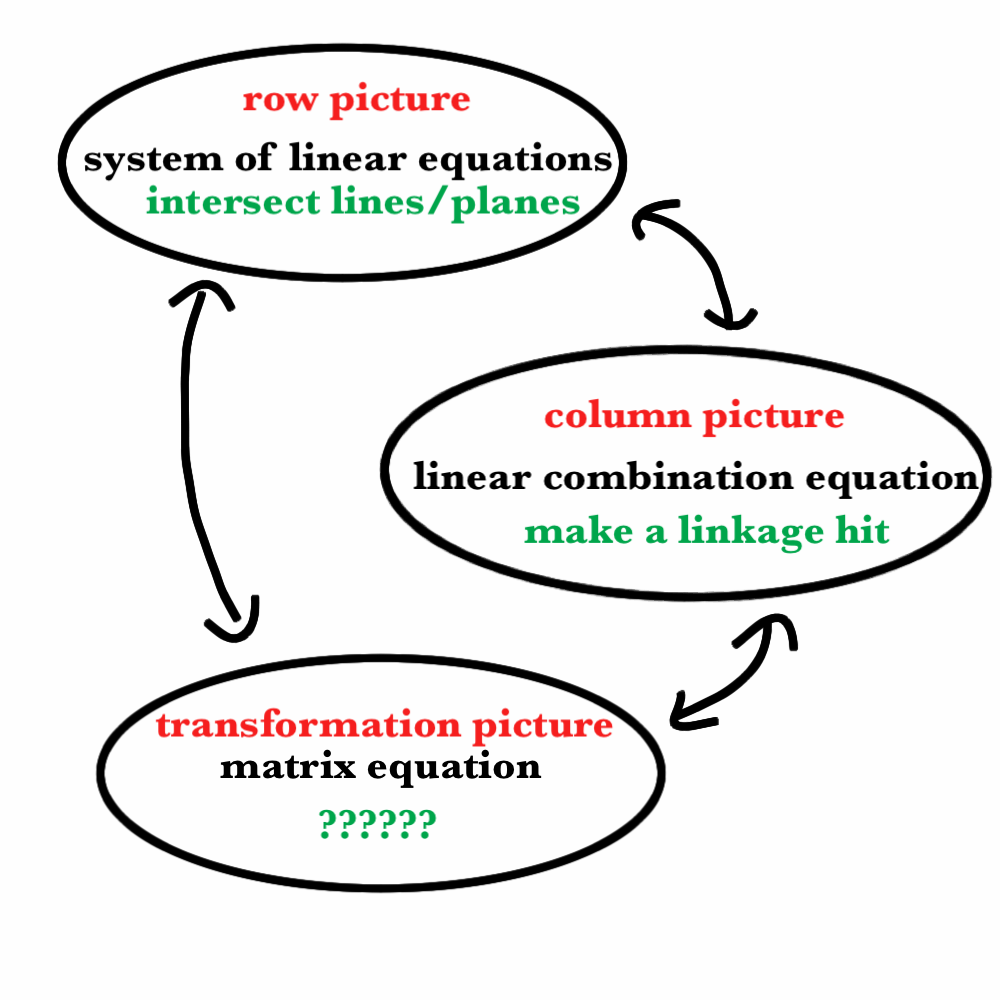
\includegraphics[width=350pt,]{images/ThreePics.png}\caption{The three geometric models of linear algebra\label{figure-1}}
\end{figure}
\par

      A deep understanding of linear algebra will involve a level of comfort with
      each of these three views of the subject in the diagram, and also the ability
      to pass back and forth between them.
    %
\typeout{************************************************}
\typeout{Subsubsection  The Transformational View}
\typeout{************************************************}
\subsubsection[The Transformational View]{The Transformational View}\label{subsubsection-10}

        We have seen that matrices can be made to "act upon" vectors by a kind of
        multiplication. In particular, if \(A\) is an \(m\times n\) matrix,
        then \(A\) can be multiplied (on the left) with a column vector of size
        \(n\), and the result is a column vector of size \(m\).
      %
\par

        This makes \(A\) into a kind of \terminology{function}. (We will use
        the synonyms \terminology{mapping} or \terminology{transformation}, too.)
        For every vector \(v\) of size \(n\), the matrix \(A\) allows
        us to compute a new vector \(T_A(v) = Av\) of size \(m\). This is
        the basic example of what we will eventually call a \terminology{linear
        transformation}.\begin{align*}
\mathbb{R}^m & \xrightarrow[]{T_A} \mathbb{R}^n\\
v & \xmapsto[]{\phantom{T_A}} Av.
\end{align*}
        One of our long term goals is to find a way to think about the geometry
        of linear algebra from this viewpoint, too.
      %
\typeout{************************************************}
\typeout{Subsection  Sage and Plotting for Linear Algebra}
\typeout{************************************************}
\subsection[Sage and Plotting for Linear Algebra]{Sage and Plotting for Linear Algebra}\label{subsection-22}
There are a few new Sage commands that might be useful here. We have
      already seen how to take linear equations and turn them into vectors
      and then turn the vector equation into a matrix equation. But Sage can
      help us move in the other direction, too.
    %
\par

      The keys are commands to pull out the rows and columns from a given matrix.
      Let's start with a simple situation where the matrix equation is
      \[
        \begin{pmatrix} 2 & 1 \\ 1 & 1 \end{pmatrix}
        \begin{pmatrix} x & y \end{pmatrix} =
        \begin{pmatrix} 3 & 4 \end{pmatrix}.
      \]
    %
\begin{lstlisting}[style=sageinput]
A = matrix(QQ, 2,2, [2,1,1,1]); A
\end{lstlisting}
\begin{lstlisting}[style=sageoutput]
[2 1]
[1 1]
\end{lstlisting}
\begin{lstlisting}[style=sageinput]
x, y = var('x y')
X = vector([x,y]); X
\end{lstlisting}
\begin{lstlisting}[style=sageoutput]
(x, y)
\end{lstlisting}
\begin{lstlisting}[style=sageinput]
b = vector([3,4]); b
\end{lstlisting}
\begin{lstlisting}[style=sageoutput]
(3, 4)
\end{lstlisting}
\par

      To get Sage to pull out the columns, we can use the \verb?.columns()?
      method. If we want just one column, we can use the \verb?.column()? method,
      but then we have to remember to specify which column we want.
    %
\begin{lstlisting}[style=sageinput]
A.columns() # this will return a list
\end{lstlisting}
\begin{lstlisting}[style=sageoutput]
[(2, 1), (1, )]
\end{lstlisting}
\begin{lstlisting}[style=sageinput]
A.column(1)
\end{lstlisting}
\begin{lstlisting}[style=sageoutput]
(1, 1)
\end{lstlisting}
\par

      \emph{Big important note:} Sage always numbers lists starting with zero.
      so the first element of every list is the \(0\) entry, and the second
      element is the \(1\) entry.
    %
\par

      Now it is possible to make Sage do things like this:
    %
\begin{lstlisting}[style=sageinput]
column_plot = plot(A.column(0), color='red')
column_plot+= plot(A.column(1), color='blue')
column_plot+= plot(b, color='purple')
show(column_plot, figsize=5, aspect_ratio=1)
\end{lstlisting}
\par

      This is an example of the a column picture.
    %
\par

      One can also pull out the rows with corresponding row methods. And if you
      recall the way that matrix multiplication works if you think of rows, you
      can make a row picture.
    %
\begin{lstlisting}[style=sageinput]
A.rows()
\end{lstlisting}
\begin{lstlisting}[style=sageoutput]
[(2, 1), (1, 1)]
\end{lstlisting}
\begin{lstlisting}[style=sageinput]
expr1 = A.row(0).dot_product(X) == b[0]
expr2 = A.row(1).dot_product(X) == b[1]

print expr1
print expr2
\end{lstlisting}
\begin{lstlisting}[style=sageoutput]
2*x + y == 3
x + y == 4
\end{lstlisting}
\par

      And now the picture:
    %
\begin{lstlisting}[style=sageinput]
row_plot = implicit_plot(expr1, [x,-5,5], [y,-1,9], color='blue')
row_plot+= implicit_plot(expr2, [x,-5,5], [y,-1,9], color='red')
show(row_plot, axes=True)
\end{lstlisting}
\typeout{************************************************}
\typeout{Subsection  Exercises}
\typeout{************************************************}
\subsection[Exercises]{Exercises}\label{subsection-23}
\begin{task}
\label{task-31}

        Make an example of a system of linear equations which some students might
        find challenging to change into an equation involving a linear combination.
        Explain what the challenge is and how you can think clearly to overcome it.
      \end{task}
\begin{task}
\label{task-32}

        Make an example of a linear combination equation which some students might
        find challenging to change into a system of linear equations. Explain
        what the challenge is and how you can think clearly to overcome it.
      \end{task}
\begin{task}
\label{task-33}

        Consider the matrix equation\[
        \begin{pmatrix}1 & 2 & 4 \\ 2 & 0 & 1 \end{pmatrix}
          \begin{pmatrix} x \\ y \\ z \end{pmatrix} = \begin{pmatrix} -1 \\ 3
          \end{pmatrix}.
        \]\begin{enumerate}
\item{}
            Draw a diagram representing the row picture of this matrix equation.
          \item{}
            Draw a diagram representing the column picture of this matrix equation.
          \end{enumerate}
\end{task}
\begin{task}
\label{task-34}

        Make an example of a system of linear equations so that the
        corresponding column picture is about linear combinations of four 2-vecs
        becoming the zero vector.
      \end{task}
\begin{task}
\label{task-35}

        Find a linear combination equation so that the corresponding system of
        linear equations corresponds to finding the intersection of three lines
        in the plane.
      \end{task}
\begin{task}
\label{task-36}

        Find an example of a vector \(b\) so that the equation\[
          \begin{pmatrix} -1 & 2 \\ 5 & -9 \end{pmatrix} v = b
        \]
        has no solution \(v\), or explain why it is impossible to find
        such an example.
      \end{task}
\begin{task}
\label{task-37}

        In each of the below, find an example of a matrix \(B\) which has the
        described effect.
        \begin{enumerate}
\item{}
            \(
              B\begin{pmatrix} x \\ y \end{pmatrix} = \begin{pmatrix}y \\ x \end{pmatrix}
            \)
          \item{}
            Rotates vectors through \(45^{\circ}\) counter-clockwise.
          \item{}
            Reflects vectors across the \(y\)axis.
          \item{}
            \(
              B\begin{pmatrix} x \\ y \end{pmatrix} =
              \begin{pmatrix} x+y \\ y \end{pmatrix}.
            \)
          \end{enumerate}
\end{task}
\clearpage
\typeout{************************************************}
\typeout{Section 2.2 Solving Systems}
\typeout{************************************************}
\section[Solving Systems]{Solving Systems}\label{elimination}
\typeout{************************************************}
\typeout{Subsection  The Assignment}
\typeout{************************************************}
\subsection[The Assignment]{The Assignment}\label{subsection-24}
\begin{itemize}
\item{}Read section 2.2 of Strang (pages 45-51).\item{}Read the following and complete the exercises below.\end{itemize}
\typeout{************************************************}
\typeout{Subsection  Learning Goals}
\typeout{************************************************}
\subsection[Learning Goals]{Learning Goals}\label{subsection-25}

      Before class, a student should be able to do the following things.
    %
\begin{itemize}
\item{}Clearly state and use the following vocabulary words: pivot, multiplier,
        triangular matrix, back substitution, singular, non-singular
      \end{itemize}
\par

      Sometime after class, a student should be able to the following things.
    %
\begin{itemize}
\item{}Perform elimination to put a system of linear equations into triangular form.\item{}Solve small systems by hand.\item{}Explain the two failure modes for elimination, and describe which leads to
        no solutions, and which leads to infinitely many solutions.\item{}Solve larger systems with the help of a computer algebra package (Sage).\end{itemize}
\typeout{************************************************}
\typeout{Subsection  Discussion: Elimination for Solving Systems of Linear Equations}
\typeout{************************************************}
\subsection[Discussion: Elimination for Solving Systems of Linear Equations]{Discussion: Elimination for Solving Systems of Linear Equations}\label{subsection-26}

        Now we begin the process of learning how to solve a system of linear
        equations systematically through a process called \terminology{elimination}.
      %
\typeout{************************************************}
\typeout{Subsubsection  Some terminology}
\typeout{************************************************}
\subsubsection[Some terminology]{Some terminology}\label{subsubsection-11}
A typical system looks something like this:
          \[
            \left\{ \begin{array}{rrrrrrrr}
                  3 x_1 & +&  2 x_2 & - & \pi x_3 & = & 0 \\
                  -4 x_1 & -& 33 x_2 & + & x_3 & = & 12
                  \end{array}\right.
          \]
          This situation is \emph{two} equations in \emph{three} unknowns.
          The unknowns here are the three numbers \(x_1\), \(x_2\) and
          \(x_3\) for which we search. Usually, we bundle the numbers
          together as a vector \((x_1, x_2, x_3)\). If we can find a vector
          which makes all of the equations true simultaneously, we call that
          vector a \terminology{solution}.
        %
\par

          Keep in mind that the process involves eliminating instances of the
          variable below \terminology{pivots}. Strang describes the process
          pretty well, and gives good examples. What Strang describes in this
          section is sometimes called \terminology{the forward pass} elimination.
        %
\par

          Watch out for situations which are \terminology{singular} in that they
          have fewer pivots than unknowns. A system is called
          \terminology{non-singular} if it has as many pivots as unknowns.
        %
\typeout{************************************************}
\typeout{Subsubsection  Keeping track of things}
\typeout{************************************************}
\subsubsection[Keeping track of things]{Keeping track of things}\label{subsubsection-12}

          Playing with all of the equations is nice, but all that really
          matters is the collection of coefficients, and the numbers on the
          right hand sides of the equal signs. Experienced solvers get tired
          of copying notation from line to line in a computation, so they only
          keep track of the matrix of coefficients, \terminology{augmented} by
          the vector on the right-hand side. In the example above, that
          augmented matrix is
          \[
            \augmatrix{ccc}{
            3 & 2 & -\pi & 0 \\ -4 & -33 & 1 & 12
            }
          \]
          All of the row operations can be performed on just this augmented
          matrix, without losing any of the essential information.
        %
\typeout{************************************************}
\typeout{Subsection  Sage and Row Operations}
\typeout{************************************************}
\subsection[Sage and Row Operations]{Sage and Row Operations}\label{subsection-27}

        The process of elimination for systems of equations involves performing
        operations on the equations. When translated to matrix form, it involves
        operations on the rows of the coefficient matrix. The corresponding
        matrix methods come in two types.
      %
\par

        The first type of method modifies the matrix ``in place'', which means
        that it \emph{Changes the input matrix}.
      %
\begin{itemize}
\item{}\verb?A.rescale_row(r, num)? multiplies row \verb?r? by the factor of \verb?num?.\item{}\verb?A.swap_rows(r1, r2)? switches the places of rows \verb?r1? and \verb?r2?.\item{}\verb?A.add_multiple_of_row(target, useful, num)?. This adds \verb?num?
          times row \verb?useful? to row \verb?target?.\end{itemize}
\par

        Throughout, please remember that Sage uses \(0\)-based indexing! So
        the rows are labeled \verb?0, 1, 2, ...?
      %
\begin{lstlisting}[style=sageinput]
A = matrix(QQ, 3,3, [0,2,4, 1,1,5, 6,2,5]); A
\end{lstlisting}
\begin{lstlisting}[style=sageoutput]
[0 2 4]
[1 1 5]
[6 2 5]
\end{lstlisting}
\begin{lstlisting}[style=sageinput]
A.swap_rows(0,1); A
\end{lstlisting}
\begin{lstlisting}[style=sageoutput]
[1 1 5]
[0 2 4]
[6 2 5]
\end{lstlisting}
\begin{lstlisting}[style=sageinput]
A.add_multiple_of_row(2,0,-6)
A # this should add -6 times row 0 to row 2
\end{lstlisting}
\begin{lstlisting}[style=sageoutput]
[  1   1   5]
[  0   2   4]
[  0  -4 -25]
\end{lstlisting}
\begin{lstlisting}[style=sageinput]
A.rescale_row(1,1/2); A
\end{lstlisting}
\begin{lstlisting}[style=sageoutput]
[  1   1   5]
[  0   1   2]
[  0  -4 -25]
\end{lstlisting}
\begin{lstlisting}[style=sageinput]
A.add_multiple_of_row(2,1,4)
A # this should add 4 times row 2 to row 2
\end{lstlisting}
\begin{lstlisting}[style=sageoutput]
[  1   1   5]
[  0   1   2]
[  0   0 -17]
\end{lstlisting}
\begin{lstlisting}[style=sageinput]
A.rescale_row(2,-1/17); A
\end{lstlisting}
\begin{lstlisting}[style=sageoutput]
[1 1 5]
[0 1 2]
[0 0 1]
\end{lstlisting}
\par

        This just did the whole process of \terminology{forward pass elimination}.
        (Well, we did a bit more than Strang would. He wouldn't rescale the rows.)
      %
\par

        Sometimes you do not want to change the matrix \verb?A?. If instead, you
        want to leave \verb?A? alone, you can use these methods, which return
        a new object and do not change \verb?A?.
      %
\begin{itemize}
\item{}\verb?A.with_rescaled_row(r, num)?\item{}\verb?A.with_swapped_rows(r1, r2)?\item{}\verb?A.with_added_multiple_of_row(t, u, num)?\end{itemize}
\par

        Let's do the same operations as above, but without changing \verb?A?.
        This will mean making a bunch of new matrices. In fact, let's also change
        the name of our matrix to \verb?B?
      %
\begin{lstlisting}[style=sageinput]
B = matrix(QQ, 3,3, [0,2,4, 1,1,5, 6,2,5]); B
\end{lstlisting}
\begin{lstlisting}[style=sageoutput]
[0 2 4]
[1 1 5]
[6 2 5]
\end{lstlisting}
\begin{lstlisting}[style=sageinput]
B1 = B.with_swapped_rows(0,1); B1
\end{lstlisting}
\begin{lstlisting}[style=sageoutput]
[1 1 5]
[0 2 4]
[6 2 5]
\end{lstlisting}
\begin{lstlisting}[style=sageinput]
B2 = B1.with_added_multiple_of_row(2,0,-6)
B2 # this should add -6 times row 0 to row 2
\end{lstlisting}
\begin{lstlisting}[style=sageoutput]
[  1   1   5]
[  0   2   4]
[  0  -4 -25]
\end{lstlisting}
\begin{lstlisting}[style=sageinput]
B3 = B2.with_rescaled_row(1,1/2); B3
\end{lstlisting}
\begin{lstlisting}[style=sageoutput]
[  1   1   5]
[  0   1   2]
[  0  -4 -25]
\end{lstlisting}
\begin{lstlisting}[style=sageinput]
B4 = B3.with_added_multiple_of_row(2,1,4)
B4 # this should add 4 times row 2 to row 2
\end{lstlisting}
\begin{lstlisting}[style=sageoutput]
[  1   1   5]
[  0   1   2]
[  0   0 -17]
\end{lstlisting}
\begin{lstlisting}[style=sageinput]
B5 = B4.with_rescaled_row(2,-1/17); B5
\end{lstlisting}
\begin{lstlisting}[style=sageoutput]
[1 1 5]
[0 1 2]
[0 0 1]
\end{lstlisting}
\par

        This second option has some advantages. At any point, you can revise your
        work, because the original matrix is still in memory, and so are all of
        the intermediate steps. Let's display all six of the matrices at once to
        see that they all still exist.
      %
\begin{lstlisting}[style=sageinput]
B, B1, B2, B3, B4, B5
\end{lstlisting}
\typeout{************************************************}
\typeout{Subsection  Exercises}
\typeout{************************************************}
\subsection[Exercises]{Exercises}\label{subsection-28}
\begin{task}
\label{task-38}

          Use the elimination method to transform this system into an easier
          one. (Can you make it triangular?) Circle the pivots in the final
          result.
          \[
            \left\{
            \begin{array}{rrrrrrr}
            2x & + & 3y & + &  z & = & 8\\
            4x & + & 7y & + & 5z & = & 20 \\
               & - & 2y & + & 2z & = & 0
            \end{array}\right.
          \]
          What two operations do you use to do this efficiently? Now use back
          substitution to solve the system.
        \end{task}
\begin{task}
\label{task-39}

            \emph{(Sage Exercise)}:
            Because the last system can be transformed in two operations, there
            are three equivalent systems generated through the process
            (the original, the intermediate, and the final).
          %
\par

            Make row picture plots for each of the three systems. [Hint: Sage]
            How do the operations transform the pictures?
          %
\end{task}
\begin{task}
\label{task-40}

          Suppose that a system of three equations in three unknowns has two
          solutions \((a,b,c)\) and \((A,B,C)\). Explain why the system must have
          other solutions than these two. Describe clearly two other solutions
          in terms of \(a,b,c,A,B,C\).
        \end{task}
\begin{task}
\label{task-41}

          Find three examples of numbers \(a\) so that elimination will fail to
          give three pivots for this coefficient matrix:
          \[
            A = \begin{pmatrix}
            a & 2 & 3 \\ a & a & 4 \\ a & a & a
            \end{pmatrix}
          \]\end{task}
\begin{task}
\label{task-42}

          How many ways can two lines in the plane meet? Make examples to
          represent as many \emph{qualitatively different} situations as you can.
        \end{task}
\begin{task}
\label{task-43}

          Complete the following to make an example of a system of two equations
          in two unknowns which is singular but still has a solution, or explain why
          no such example exists.
          \[
            \left\{
            \begin{array}{ccccc}
            2x & + & 3y & = & 1 \\
            \bullet x & + & \bullet y & = & \bullet
            \end{array}\right.
          \]\end{task}
\begin{task}
\label{task-44}

          Complete the following to a system of three equations in three
          unknowns which is singular and does not have a solution, or explain
          why no such example exists.
          \[
            \left\{
            \begin{array}{ccccccc}
               &  & 3y & - & z & = & 1 \\
            2x & - & y & + & 3z & = & 0 \\
            \bullet x & + & \bullet y & + &\bullet z &  = & \bullet
            \end{array}\right.
          \]\end{task}
\begin{task}
\label{task-45}

          Complete the following to a system of three equations in three
          unknowns which is singular but still has a solution, or explain why
          no such example exists.
          \[
            \left\{
            \begin{array}{ccccccc}
            x & + & y & + & z & = & 1 \\
            2x & + & y & + & 2z & = & 0 \\
            \bullet x & + & \bullet y & + &\bullet z &  = & \bullet
            \end{array}\right.
          \]\end{task}
\begin{task}
\label{task-46}

          How many ways can three planes in three dimensional space meet? Make
          examples to represent as many \emph{qualitatively different}
          situations as you can.
        \end{task}
\clearpage
\typeout{************************************************}
\typeout{Section 2.3 Elimination using Matrices}
\typeout{************************************************}
\section[Elimination using Matrices]{Elimination using Matrices}\label{matrix-elimination}
\typeout{************************************************}
\typeout{Subsection  The Assignment}
\typeout{************************************************}
\subsection[The Assignment]{The Assignment}\label{subsection-29}
\begin{itemize}
\item{}Read section 2.3 of \emph{Strang}.\item{}Read the discussion below and work out the exercises.\end{itemize}
\typeout{************************************************}
\typeout{Subsection  Learning Goals}
\typeout{************************************************}
\subsection[Learning Goals]{Learning Goals}\label{subsection-30}

        Before class, a student should be able to:
      %
\begin{itemize}
\item{}
          Translate a system of linear equations into the form of an augmented matrix
          and back.
        \item{}
          Perform the forward pass elimination process to an augmented matrix.
        \item{}
          Multiply a pair of square matrices having the same size.
        \item{}
          Identify the matrix which performs the operation ``add a multiple of row
          i to row j.''
        \item{}Identify the matrix which performs the operation ``swap the places of
          row i and row j.''
        \end{itemize}
\par

        Some time after class, a student should be able to:
      %
\begin{itemize}
\item{}
          Use the steps from a forward pass elimination step to write a correct
          equation of the form
          \[
            E_{\bullet}E_{\bullet}\cdots E_{\bullet} (A\ |\ b) = (U\ |\ b')
          \]
          where \(U\) is an upper triangular matrix.
        \end{itemize}
\typeout{************************************************}
\typeout{Subsection  Discussion: Elimnation and Using Matrices as ``Transformations''}
\typeout{************************************************}
\subsection[Discussion: Elimnation and Using Matrices as ``Transformations'']{Discussion: Elimnation and Using Matrices as ``Transformations''}\label{subsection-31}

      Let us focus (for now) on square systems of equations, where the number of
      unknowns is equal to the number of equations.
    %
\typeout{************************************************}
\typeout{Subsubsection  The Four Ways to Write a System}
\typeout{************************************************}
\subsubsection[The Four Ways to Write a System]{The Four Ways to Write a System}\label{subsubsection-13}

        Recall that there are three equivalent ways to write the typical linear
        algebra problem: (1) a system of linear equations to be solved
        simultaneously, (2) an equation expressing some linear combination of
        vectors with unknown coefficients as equal to another vector, and (3) a
        matrix equation.
      %
\par

        Here is an example: This system of linear equations
        \[
          \left\{ \begin{array}{rrrrrrr}
              &  &3y &+ &2z &= &8 \\
            x &- & y &+ & z &= &-1 \\
          3 x &+ &2y &+ &3z &= &1
          \end{array}\right.
        \]
        is equivalent to this equation using a linear combination of vectors
        \[
        x \begin{pmatrix} 0 \\ 1 \\ 3 \end{pmatrix} +
        y \begin{pmatrix} 3 \\ -1 \\ 2 \end{pmatrix} +
        z \begin{pmatrix} 2 \\ 1 \\ 3 \end{pmatrix} =
        \begin{pmatrix} 8 \\ -1 \\ 1 \end{pmatrix}
        \]
        and both of those are equivalent to this matrix equation
        \[
          \begin{pmatrix} 0 &3 &2 \\ 1 &-1 &1 \\ 3 &2 &3
          \end{pmatrix} \begin{pmatrix} x \\ y \\ z \end{pmatrix} =
          \begin{pmatrix} 8 \\ -1 \\ 1 \end{pmatrix} .
        \]
      %
\par

        Each of these viewpoints has its advantages when talking about the
        geometry of linear algebra. But one way that things steadily improve as
        you move down the page is in the amount of notational baggage.
        From each version to the next, we lose repetitive bits of symbol that
        one can just remember from context.
        Often, this is taken one step further! We now throw away the unknowns,
        the equal signs and some of the parentheses surrounding the matrices and
        vectors, and just write an \emph{augmented} matrix.
        \[
          \augmatrix{ccc}{
          0 &3 &2 &8\\ 1 &-1 &1 &-1\\ 3 &2 &3 &1
          }
        \]
        This is the minimum fuss way to keep track of all the information you
        need to solve the original system.
      %
\typeout{************************************************}
\typeout{Subsubsection  Representing Elimination with Matrices}
\typeout{************************************************}
\subsubsection[Representing Elimination with Matrices]{Representing Elimination with Matrices}\label{subsubsection-14}

        The process of elimination starts by performing operations on the
        system of equations. In the example above, one simplification we can
        make is to add \(-3\) times equation (ii) to equation (iii).
      %
\par

        Then the new system looks like this:
        \[
          \left\{ \begin{array}{rrrrrrr}
          &  &3y &+ &2z &= &8 \\
          x &- & y &+ & z &= &-1 \\
          &  &5y &  &   &= &4
          \end{array}\right.
        \]
        Let's translate that into the linear combination format:
        \[
          x \begin{pmatrix} 0 \\ 1 \\ 0 \end{pmatrix} +
          y \begin{pmatrix} 3 \\ -1 \\ 5 \end{pmatrix} +
          z \begin{pmatrix} 2 \\ 1 \\ 0 \end{pmatrix} =
          \begin{pmatrix} 8 \\ -1 \\ 4 \end{pmatrix} .
        \]
        What has happened to each of the vectors? Well, in each case, we have
        added \(-3\) times the second component to the third component.
        We have seen that one way to change vectors into other vectors is by
        (left-)multiplying them by matrices. Could we be so lucky that the
        operation ``add \(-3\) times the second component to the third
        component'' is representable by a matrix operation? YES. It is not
        hard to check that the matrix we need is
        \[
          E = \begin{pmatrix} 1 &0 &0 \\ 0 &1 &0 \\ 0 &-3 &1 \end{pmatrix} .
        \]
        In fact, let's check it now for each of the four vectors we have in our system:
        \[
          E \begin{pmatrix} 0 \\ 1 \\ 3 \end{pmatrix} =
          \begin{pmatrix} 1 &0 &0 \\ 0 &1 &0 \\
          0 &-3 &1 \end{pmatrix} \begin{pmatrix} 0 \\ 1 \\ 3 \end{pmatrix}
          = \begin{pmatrix} 0 \\ 1 \\ 0 \end{pmatrix}
        \]
        and
        \[
          E \begin{pmatrix} 3 \\ -1 \\ 2 \end{pmatrix} =
          \begin{pmatrix} 1 &0 &0 \\ 0 &1 &0 \\ 0 &-3
          &1 \end{pmatrix} \begin{pmatrix} 3 \\ -1 \\ 2 \end{pmatrix} =
          \begin{pmatrix} 3 \\ -1 \\ 5 \end{pmatrix}
        \]
        and
        \[
          E \begin{pmatrix} 2 \\ 1 \\ 3 \end{pmatrix} =
          \begin{pmatrix} 1 &0 &0 \\ 0 &1 &0 \\
          0 &-3 &1 \end{pmatrix} \begin{pmatrix} 2 \\ 1 \\ 3
          \end{pmatrix} = \begin{pmatrix} 2 \\ 1 \\ 0 \end{pmatrix}
        \]
        and
        \[
          E \begin{pmatrix} 8 \\ -1 \\ 1 \end{pmatrix} =
          \begin{pmatrix} 1 &0 &0 \\ 0 &1 &0 \\
          0 &-3 &1 \end{pmatrix} \begin{pmatrix} 8 \\ -1 \\ 1 \end{pmatrix}
          = \begin{pmatrix} 8 \\ -1 \\ 4 \end{pmatrix}.
        \]
      %
\par

        Ha Ha! It all checks out. Those are the four vectors from our second
        system. This means that we can even use a simple subsitution to rewrite
        things. (It is not obvious at the moment why this is helpful. Hang on a
        bit.)
        \[
          x* E\begin{pmatrix} 0 \\ 1 \\ 3 \end{pmatrix} +
          y* E\begin{pmatrix} 3 \\ -1 \\ 2 \end{pmatrix} +
          z* E\begin{pmatrix} 2 \\ 1 \\ 3 \end{pmatrix} =
          E\begin{pmatrix} 8 \\ -1 \\ 1 \end{pmatrix}
        \]
        Boy, it sure would be nice if we had a compact way to write that down...
      %
\typeout{************************************************}
\typeout{Subsubsection  Matrix Multiplication}
\typeout{************************************************}
\subsubsection[Matrix Multiplication]{Matrix Multiplication}\label{subsubsection-15}

        We make a compact way to write down that last equation by defining an
        operation of multiplying two matrices.
        If \(E\) and \(A\) are two matrices, we define their
        \terminology{matrix product}
        to be a new matrix as follows:
      %
\par

        First, write \(A\) as a collection of columns \(v_i\)
        \[
          A = \begin{pmatrix} v_1 &v_2 &v_3 \end{pmatrix}
        \]
        and then we declare that \(EA\) is the matrix made up of the columns
        \(Ev_i\) in the corresponding order.
        \[
          EA = \begin{pmatrix} Ev_1 &Ev_2 &Ev_3 \end{pmatrix}
        \]
      %
\par

        By way of example, we have already considered the matrices
        \[
          E = \begin{pmatrix} 1 &0 &0 \\ 0 &1 &0 \\ 0 &-3 &1 \end{pmatrix} \quad \text{ and } \quad
          A = \begin{pmatrix} 0 &3 &2 \\ 1 &-1 &1 \\ 3 &2 &3 \end{pmatrix}.
        \]
        You should check that their product is now
        \[
          EA = \begin{pmatrix} 1 &0 &0 \\ 0 &1 &0 \\ 0 &-3 &1 \end{pmatrix}\begin{pmatrix} 0 &3 &2 \\ 1 &-1 &1 \\ 3 &2 &3 \end{pmatrix} =
          \begin{pmatrix} 0 &3 &2 \\ 1 &-1 &1 \\ 0 &5 &0 \end{pmatrix}
        \]
      %
\par

        Finally, let's see how this influences our last two forms of the equations.
        The matrix form of our system was \(Ax = v\) where \(A\) is as above, and the
        vectors are \(v = \left(\begin{smallmatrix} 8 \\ -1 \\ 1
        \end{smallmatrix}\right)\) and
        \(x = \left( \begin{smallmatrix} x \\ y \\ z \end{smallmatrix}\right)\).
        The neat part is that our new definition of matrix multiplication means
        that our elimination step transformed the equation
        \[
          Ax = v \quad \text{ or }\quad
          \begin{pmatrix} 0 &3 &2 \\ 1 &-1 &1 \\ 3 &2 &3
          \end{pmatrix} \begin{pmatrix} x \\ y \\ z \end{pmatrix} =
          \begin{pmatrix} 8 \\ -1 \\ 1 \end{pmatrix}
        \]
        into the newer equation
        \[
          (EA) x = Ev \quad \text{ or } \quad \begin{pmatrix} 0 &3 &2
          \\ 1 &-1 &1 \\ 0 &5 &0 \end{pmatrix} \begin{pmatrix} x
          \\ y \\ z \end{pmatrix} = \begin{pmatrix} 8 \\ -1 \\ 4 \end{pmatrix}.
        \]
      %
\par

        The same thing works for the augmented matrix. The augmented matrix form
        is really just writing down
        \[
          \augmatrix{c}{A &v }
          =\augmatrix{ccc}{
          0 &3 &2 &8\\ 1 &-1 &1 &-1\\ 3 &2 &3 &1 }
        \]
        and the elimination step changes this into
        \[
          \augmatrix{c}{EA &Ev}
          = \augmatrix{ccc}{
          0 &3 &2 &8 \\ 1 &-1 &1 &-1 \\ 0 &5 &0 &4
          }.
        \]
      %
\typeout{************************************************}
\typeout{Subsubsection  Matrices as Transformations}
\typeout{************************************************}
\subsubsection[Matrices as Transformations]{Matrices as Transformations}\label{subsubsection-16}

        Take a moment and reflect on the key transition in what happens above.
        The most important thing that made it all work was that a matrix (the
        elimination matrix \(E\)) was used to perform some sort of operation on
        vectors.
      %
\par

        This is a key property of matrices. The matrix \(E\) defines a kind of
        function. For every vector \(w\) with three components, we can compute
        exactly one new vector \(Ew\), still with three components. This means that
        \(E\) defines a function from the set of \(3\)-vectors to the set of
        \(3\)-vectors.
      %
\typeout{************************************************}
\typeout{Subsection  Sage and Matrix Multiplication}
\typeout{************************************************}
\subsection[Sage and Matrix Multiplication]{Sage and Matrix Multiplication}\label{subsection-32}

      Sage has built-in matrix multiplication. You do the obvious thing and it
      works.
    %
\begin{lstlisting}[style=sageinput]
A = matrix(QQ, 2,2, [[2,1],[1,1]])
B = matrix(QQ, 2,2, [[0,3],[1,1]])
A, B
\end{lstlisting}
\begin{lstlisting}[style=sageoutput]
(
[2 1]  [0 3]
[1 1], [1 1]
)
\end{lstlisting}
\begin{lstlisting}[style=sageinput]
A*B
\end{lstlisting}
\par

      You can check that it works with the way we defined matrix multiplication
      as a linear combination of vectors, too.
    %
\par

      First, we define the column vectors by pulling out the entries from \verb?B?
      and arranging them. To be sure, we ask Sage to display them as columns.
    %
\begin{lstlisting}[style=sageinput]
b1 = vector([B[0,0], B[1,0]])
b2 = vector([B[0,1], B[1,1]])
b1.column(), b2.column()
\end{lstlisting}
\begin{lstlisting}[style=sageoutput]
(
[0]  [3]
[1], [1]
)
\end{lstlisting}
\begin{lstlisting}[style=sageinput]
A*b1.column(), A*b2.column()
\end{lstlisting}
\begin{lstlisting}[style=sageoutput]
(
[1]  [7]
[1], [4]
)
\end{lstlisting}
\par

      Now we can pile these rows into a matrix and then use the transpose to
      put them in columns.
    %
\begin{lstlisting}[style=sageinput]
C = matrix([A*b1, A*b2]).transpose()
C
\end{lstlisting}
\begin{lstlisting}[style=sageoutput]
[1 7]
[1 4]
\end{lstlisting}
\par

      And we can double check everything by asking Sage if these things are equal.
    %
\begin{lstlisting}[style=sageinput]
C == A*B
\end{lstlisting}
\begin{lstlisting}[style=sageoutput]
True
\end{lstlisting}
\par

      This kind of test can be useful for checking our work! The discussion above
      has this multiplication:
    %
\begin{lstlisting}[style=sageinput]
D = matrix(QQ,3,4, [0,3,2,8,1,-1,1,-1,3,2,3,1]); D
\end{lstlisting}
\begin{lstlisting}[style=sageoutput]
[ 0  3  2  8]
[ 1 -1  1 -1]
[ 3  2  3  1]
\end{lstlisting}
\begin{lstlisting}[style=sageinput]
E = matrix.identity(3)
E[2,1] = -3
E
\end{lstlisting}
\begin{lstlisting}[style=sageoutput]
[ 1  0  0]
[ 0  1  0]
[ 0 -3  1]
\end{lstlisting}
\begin{lstlisting}[style=sageinput]
E*D
\end{lstlisting}
\begin{lstlisting}[style=sageoutput]
[ 0  3  2  8]
[ 1 -1  1 -1]
[ 0  5  0  4]
\end{lstlisting}
\par

      Ta-Da!!!
    %
\typeout{************************************************}
\typeout{Subsection  Exercises}
\typeout{************************************************}
\subsection[Exercises]{Exercises}\label{subsection-33}
\begin{task}
\label{task-47}

      In the main example above
      \[
      \left\{ \begin{array}{rrrrrrr}
         &  &3y &+ &2z &= &8 \\
       x &- & y &+ & z &= &-1 \\
      3x &+ &2y &+ &3z &= &1
      \end{array}
      \right.
      \]
      we would rather have our first pivot in the upper left corner (i.e. the
      first row should have a non-zero coefficient for \(x\)). This can be
      achieved by swapping the positions of rows (i) and (ii).
    %
\par

      Find a matrix \(P_{12}\) so that multiplying by \(P_{12}\) on the left
      performs the corresponding row switching operation on the augmented matrix
      \[
      \augmatrix{ccc}{
      0 &3 &2 &8 \\ 1 &-1 &1 &-1 \\ 3 &2 &3 &1}
      \]
    %
\end{task}
\begin{task}
\label{task-48}

      Consider the system
      \[
      \left\{ \begin{array}{rrrrr}
      6x &- &y &= &14 \\
      97x &- &16y &= &2/3 \\
      \end{array}
      \right.
      \]
      Write this system in the other three forms: (1) an equation involving a
      linear combination of vectors; (2) an equation involving a \(2\times 2\)
      matrix; (3) an augmented matrix.
    %
\end{task}
\begin{task}
\label{task-49}

      Perform an elimination step on the system from the last exercise to put the sytem in triangular form. You should get two pivots.
    %
\par

      Write the new system in each of our four forms.
    %
\end{task}
\begin{task}
\label{task-50}

      Still working with the same system of equations, use Sage to make two column picture plots:
    %
\begin{itemize}
\item{} One showing the three relevant column vectors from the original system.\item{} One showing the three relevant column vectors from the system after the elimination step.\end{itemize}
\par

      You may find it helpful to look through the Sage examples in previous sections
      of this workbook.
    %
\end{task}
\begin{task}
\label{task-51}

      One more time, stay with the same system of equations. Use Sage to make
      two row picture plots:
    %
\begin{itemize}
\item{} One showing the two relevant lines in the original system.\item{} One showing the two relevant lines from the system after the elimination step.\end{itemize}
\par

      You may find it helpful to look through the Sage examples in previous sections
      of this workbook.
    %
\end{task}
\begin{task}
\label{task-52}

      Consider this system of three equations in three unknowns:
      \[
      \left\{
      \begin{array}{rrrrrrr}
      -x &+ &\frac{2}{3} y &+ &z &= &1 \\
       x &+ &           6y &+ &z &= &1 \\
      3x &  &              &+ &3z&= &1 \\
      \end{array}\right.
      \]
      Perform the elimination steps to transform this system into a triangular one.
    %
\par

      Write down the corresponding matrices you use to perform each of these
      steps on the augmented matrix version of this system.
    %
\end{task}
\begin{task}
\label{task-53}

      Still working with the system of equations from the last task, use Sage
      to make two column picture plots:
    %
\begin{itemize}
\item{} One showing the four relevant column vectors from the original system.\item{} One showing the four relevant column vectors from the system after the elimination step.\end{itemize}
\par

      You may find it helpful to look through the Sage examples in previous sections
      of this workbook.
    %
\end{task}
\begin{task}
\label{task-54}

      One more time, stay with the system of equations from previous two tasks.
      Use Sage to make two row picture plots:
    %
\begin{itemize}
\item{} One showing the two relevant lines in the original system.\item{} One showing the two relevant lines from the system after the elimination step.\end{itemize}
\par

      You may find it helpful to look through the Sage examples in previous sections
      of this workbook.
    %
\end{task}
\clearpage
\typeout{************************************************}
\typeout{Section 2.4 Going Further with Elimination}
\typeout{************************************************}
\section[Going Further with Elimination]{Going Further with Elimination}\label{lin-eq-going-further-1}
\typeout{************************************************}
\typeout{Subsection  The Assignment}
\typeout{************************************************}
\subsection[The Assignment]{The Assignment}\label{subsection-34}
\begin{itemize}
\item{}
        Go back through the exercises in the first three sections of this chapter.
        Complete any items you
        did not complete the first time through. Prepare any that we have not
        discussed in class so that you will be ready to present them.
      \end{itemize}
\typeout{************************************************}
\typeout{Subsection  Discussion}
\typeout{************************************************}
\subsection[Discussion]{Discussion}\label{subsection-35}
Now we take a short break to revisit and consolidate the learning you
      have done so far. Revisit the reading and the exercises you have done in
      Chapter Two: Linear Equations. The important feature of this work should be
      learning to think about your own thinking. This sort of \terminology{meta-cognition}
      characterizes expert learners. Eventually, you want to be able to monitor
      your work at all times and recognize when you understand deeply and when
      you do not. This will allow you to self-correct.
    %
\par
To help you get started with meta-cognition, I listed learning goals in
      each section. To go further, you need to explicitly go through the process
      of reviewing what you can do and what you cannot. Here are some prompts to
      help you get started with this process.
      \begin{itemize}
\item{}
          Review the learning goals from each section. Can you do the things
          described? Can you do them sometimes, or have you mastered them so you
          can do them consistently?
        \item{}
          Look through all of the tasks and go deeper into them. Can you
          connect each exercise to one of our pictures? Try to build a mental
          model of how the exercise and its solution work.
        \item{}
          If your first solution to an exercise involve a ``guess-and-check''
          approach, can you now complete the exercise in a \emph{purposeful}
          and systematic manner?
        \item{}
          Make a list of concepts or exercises that are not clear to you. Phrase
          each item in your list as a question, and make each question as
          specific as possible. Talk with fellow students or your
          instructor until you can answer your own questions.
        \end{itemize}

    %
\clearpage
\typeout{************************************************}
\typeout{Section 2.5 Matrix Algebra}
\typeout{************************************************}
\section[Matrix Algebra]{Matrix Algebra}\label{matrix-algebra}
\typeout{************************************************}
\typeout{Subsection  The Assignment}
\typeout{************************************************}
\subsection[The Assignment]{The Assignment}\label{subsection-36}
\begin{itemize}
\item{}Read section 2.4 of \emph{Strang}.\item{}Read the following and complete the exercises below.\end{itemize}
\typeout{************************************************}
\typeout{Subsection  Learning Goals}
\typeout{************************************************}
\subsection[Learning Goals]{Learning Goals}\label{subsection-37}

      Before class, a student should be able to:
    %
\begin{itemize}
\item{}Add and subtract matrices of the same size.\item{}Multiply matrices of appropriate sizes by one method.\item{}Compute powers \(A^p\) of a given square matrix \(A\).\item{}Use the distributive law for matrix multiplication and matrix addition correctly.\end{itemize}
\par

      Sometime after our meeting, a student should be able to:
    %
\begin{itemize}
\item{}Multiply block matrices.\item{}Multiply matrices by \emph{three} methods.\item{}Give examples to show how matrix multiplication is not like
        ordinary multiplication of real numbers: including the trouble
        with commutativity, and the difficulty with inverses.
      \end{itemize}
\typeout{************************************************}
\typeout{Subsection  Discussion on Matrix Algebra}
\typeout{************************************************}
\subsection[Discussion on Matrix Algebra]{Discussion on Matrix Algebra}\label{subsection-38}

      At the simplest level, this section is just about how to deal with the
      basic operations on matrices. We can add them and we can multiply them.
      We have already encountered matrix multiplication, and addition is even
      more natural.
    %
\par

      But a subtle and important thing is happening here. Matrices are taking
      on a life of their own. They are becoming first class objects, whose
      properties are interesting and possibly useful.
    %
\par

      This is an instance of the beginnings of \emph{Modern Algebra}, which
      is the study of the algebraic structures of abstracted objects. In this
      case, we study whole collections of matrices of a common shape, and we
      try to treat them like generalized numbers. Then the natural questions
      are how much like ``regular numbers'' are these matrices?
    %
\par

      Addition is about as well-behaved as you can expect, but multiplication
      is a bit trickier. Suddenly, two properties of multiplication for numbers
      don't quite work for matrices:
    %
\begin{itemize}
\item{}multiplication does not necessarily commute: It need not be the case
        that \(AB\) is the same as \(BA\).
      \item{}we may not always have inverses: just because there is a
        matrix \(A\) which is not the zero matrix, it may not be the case
        that we can make sense of \(A^{-1}\) and get \(AA^{-1} = I\).
      \end{itemize}
\typeout{************************************************}
\typeout{Subsection  Sage and Matrix Algebra}
\typeout{************************************************}
\subsection[Sage and Matrix Algebra]{Sage and Matrix Algebra}\label{subsection-39}

      Sage is aware of the basic matrix operations, and it won't let you get
      away with nonsense. Matrix multiplication and matrix addition are only
      defined if the dimensions of the matrices line up properly.
    %
\begin{lstlisting}[style=sageinput]
A = matrix(QQ, 2,3, [0,1,2,3,6,6])# A 2 by 3 matrix
B = matrix(QQ, 2,2, [4,2,3,1]) # 2 by 2 square matrix
C = matrix(QQ, 3,3, [2,1,2,1,2,1,2,1,2]) # a 3 by 3 square matrix
D = matrix(QQ, 2,3, [1,1,1,1,1,1]) # another 2 by 3 matrix
E = matrix(QQ, 3,2, [3,4,2,5,6,1]) # a 3 by 2 matrix
\end{lstlisting}
\par

      Let's see which of these Sage doesn't like. Can you predict, before
      evaluating the cells below, which of these will return an error?
    %
\begin{lstlisting}[style=sageinput]
A*B
\end{lstlisting}
\begin{lstlisting}[style=sageinput]
B*A
\end{lstlisting}
\begin{lstlisting}[style=sageoutput]
[ 6 16 20]
[ 3  9 12]
\end{lstlisting}
\begin{lstlisting}[style=sageinput]
A+B
\end{lstlisting}
\begin{lstlisting}[style=sageinput]
A*C
\end{lstlisting}
\begin{lstlisting}[style=sageoutput]
[ 5  4  5]
[24 21 24]
\end{lstlisting}
\begin{lstlisting}[style=sageinput]
C*A
\end{lstlisting}
\begin{lstlisting}[style=sageinput]
A*D
\end{lstlisting}
\begin{lstlisting}[style=sageinput]
A+D
\end{lstlisting}
\typeout{************************************************}
\typeout{Subsubsection  Sage and Matrix Addition}
\typeout{************************************************}
\subsubsection[Sage and Matrix Addition]{Sage and Matrix Addition}\label{subsubsection-17}
Matrix addition works a lot like addition of integers, as long as you fix
        a size first.%
\begin{itemize}
\item{}There is a zero element.\item{}There are additive inverses (i.e. \emph{negatives}).\item{}The operation is commutative.\end{itemize}
\begin{lstlisting}[style=sageinput]
#This constructs the zero matrix
Z = zero_matrix(2,3); Z
\end{lstlisting}
\begin{lstlisting}[style=sageoutput]
[0 0 0]
[0 0 0]
\end{lstlisting}
\par
Let us add \verb?A? and \verb?Z?:%
\begin{lstlisting}[style=sageinput]
A + Z
\end{lstlisting}
\begin{lstlisting}[style=sageoutput]
[0 1 2]
[3 6 6]
\end{lstlisting}
\par
We can check that adding \verb?Z? doesn't change anything.%
\begin{lstlisting}[style=sageinput]
A + Z == A
\end{lstlisting}
\begin{lstlisting}[style=sageoutput]
True
\end{lstlisting}
\par
And we can do the natural thing to get an additive inverse.%
\begin{lstlisting}[style=sageinput]
L = -A; L
\end{lstlisting}
\begin{lstlisting}[style=sageoutput]
[ 0 -1 -2]
[-3 -6 -6]
\end{lstlisting}
\par
Finally, this last thing should return zero.%
\begin{lstlisting}[style=sageinput]
A + L
\end{lstlisting}
\begin{lstlisting}[style=sageoutput]
[0 0 0]
[0 0 0]
\end{lstlisting}
\typeout{************************************************}
\typeout{Subsubsection  Sage and Matrix Multiplication}
\typeout{************************************************}
\subsubsection[Sage and Matrix Multiplication]{Sage and Matrix Multiplication}\label{subsubsection-18}

        Sage already has the structure of matrix multiplication built-in, and
        it can help with investigating the ways that matrix multiplicaiton
        is different from regular multiplication of numbers.
      %
\par

        We have seen above
        that Sage will not let us multiply matrices whose sizes do not match
        correctly.  Of course, one way around that trouble is to stick to square
        matrices. But even there we can have trouble with the fact that matrix
        multiplication might not commute. It is rarely the case that \(XY = YX\).
      %
\par

        For those of you who will eventually study Modern Algebra, the collection
        of all \(n\)-square matrices is an example of a non-commutative ring
        with unit.
      %
\begin{lstlisting}[style=sageinput]
A*E, E*A
\end{lstlisting}
\begin{lstlisting}[style=sageoutput]
(
         [12 27 30]
[14  7]  [15 32 34]
[57 48], [ 3 12 18]
)
\end{lstlisting}
\par
Sage knows about the ring structure. We can check for an inverse.%
\begin{lstlisting}[style=sageinput]
B.is_invertible()
\end{lstlisting}
\begin{lstlisting}[style=sageoutput]
True
\end{lstlisting}
\begin{lstlisting}[style=sageinput]
C.is_invertible()
\end{lstlisting}
\begin{lstlisting}[style=sageoutput]
False
\end{lstlisting}
\par
And we can ask for the inverse in a couple of ways.%
\begin{lstlisting}[style=sageinput]
B.inverse()
\end{lstlisting}
\begin{lstlisting}[style=sageoutput]
[-1/2   1]
[ 3/2  -2]
\end{lstlisting}
\begin{lstlisting}[style=sageinput]
B^(-1)
\end{lstlisting}
\begin{lstlisting}[style=sageoutput]
[-1/2   1]
[ 3/2  -2]
\end{lstlisting}
\par
One can even construct the whole ring of all \(n\times n\) matrices
      and play around inside it.%
\begin{lstlisting}[style=sageinput]
M = MatrixSpace(QQ, 2,2); M
\end{lstlisting}
\begin{lstlisting}[style=sageoutput]
Full MatrixSpace of 2 by 2 dense matrices over Rational Field
\end{lstlisting}
\par
It is then not too hard to construct the identity element, which is
        the regular identity matrix of the correct size.
      %
\begin{lstlisting}[style=sageinput]
M(1)
\end{lstlisting}
\begin{lstlisting}[style=sageoutput]
[1 0]
[0 1]
\end{lstlisting}
\par
Also, the zero matrix of the correct size is easy to make.%
\begin{lstlisting}[style=sageinput]
M(0)
\end{lstlisting}
\begin{lstlisting}[style=sageoutput]
[0 0]
[0 0]
\end{lstlisting}
\par

        In fact, this allows you to short cut the construction of any matrix in
        \verb?M?. This can be really useful if you are going to work with a lot
        of matrices of the same shape.
      %
\begin{lstlisting}[style=sageinput]
H = M([2,1,1,1]); H
\end{lstlisting}
\begin{lstlisting}[style=sageoutput]
[2 1]
[1 1]
\end{lstlisting}
\par
You can even use this to make complicated expressions out of matrix operations.
        As long as everything makes sense, Sage will do all the work.
      %
\begin{lstlisting}[style=sageinput]
H^2 + H
\end{lstlisting}
\begin{lstlisting}[style=sageoutput]
[7 4]
[4 3]
\end{lstlisting}
\begin{lstlisting}[style=sageinput]
H * (H - 5*M(1) + 2*H^2)
\end{lstlisting}
\begin{lstlisting}[style=sageoutput]
[21 14]
[14  7]
\end{lstlisting}
\begin{lstlisting}[style=sageinput]
# this one should turn out to be zero.
# I know this because of a theorem.
H^2 - 3*H + M(1)
\end{lstlisting}
\begin{lstlisting}[style=sageoutput]
[0 0]
[0 0]
\end{lstlisting}
\typeout{************************************************}
\typeout{Subsubsection  Sage and Block Matrices}
\typeout{************************************************}
\subsubsection[Sage and Block Matrices]{Sage and Block Matrices}\label{subsubsection-19}
Sage has a built-in method for constructing matrices out of blocks, too.
        It is easiest to see an example.
      %
\par

        To make this work, you have to tell Sage when you have a vector if you
        want it to be either a row or a column vector in the appropriate places.
      %
\begin{lstlisting}[style=sageinput]
X = matrix(QQ, 2,2, [0,-1,1,0])
v = vector([2,3])
w = matrix(QQ, 1,1, [1])
Blockey = block_matrix(QQ, 2,3,
                       [[X, X, v.column()],
                       [v.row(), v.row(), w]])
Blockey
\end{lstlisting}
\begin{lstlisting}[style=sageoutput]
[ 0 -1| 0 -1| 2]
[ 1  0| 1  0| 3]
[-----+-----+--]
[ 2  3| 2  3| 1]
\end{lstlisting}
\typeout{************************************************}
\typeout{Subsection  Exercises}
\typeout{************************************************}
\subsection[Exercises]{Exercises}\label{subsection-40}
\begin{task}
\label{task-55}

        Make an example of a \(2\times 3\) matrix and a \(3\times 3\)
        matrix, and use this to demonstrate the three different ways to multiply
        matrices.
      \end{task}
\begin{task}
\label{task-56}

        Give an example of a pair of \(2\times 2\) matrices \(A\) and
        \(B\) so that \(AB = 0\) but \(BA\neq 0\), or explain why
        this is  impossible.
      \end{task}
\begin{task}
\label{task-57}

        Give an example of a \(3\times 3\) matrix \(A\) such that neither
        \(A\) nor \(A^2\) is the zero matrix, but \(A^3=0\).
      \end{task}
\begin{task}
\label{task-58}

        Find all examples of matrices \(A\) which commute with both
        \(B = \left( \begin{smallmatrix} 1 & 0 \\ 0 & 0
          \end{smallmatrix}\right)\) and
        \(C = \left( \begin{smallmatrix} 0 & 1 \\ 0 & 0
          \end{smallmatrix}\right)\). That is, find all matrices \(A\)
        so that \(AB = BA\) and \(AC= CA\). How do you know you have
        all such matrices?
      \end{task}
\begin{task}
\label{task-59}

          Consider the matrix
          \[
            A = \begin{pmatrix} 2 & 1 & 0 \\ -2 & 0 & 1 \\ 8 & 5 & 3 \end{pmatrix}.
          \]
          Which elimination matrices \(E_{21}\) and \(E_{31}\) produce zeros in the
          \((2,1)\) and \((3,1)\) positions of \(E_{21}A\)
          and \(E_{31}A\)?
        %
\par

          Find a single matrix \(E\) which produces both zeros at once.
          Multiply \(EA\) to verify your result.
        %
\end{task}
\begin{task}
\label{task-60}

          Let's take a different view of the last computation.
          Block multiplication says that column 1 is eliminated by
          a step that looks like this one:
          \[
            EA = \begin{pmatrix} 1 & 0 \\ -c/a & I \end{pmatrix}
            \begin{pmatrix} a & b \\ c & D \end{pmatrix} =
            \begin{pmatrix} a & b \\ 0 & D - cb/a \end{pmatrix}.
          \]
          Here \(I\) is the \(2\times 2\) identity matrix, \(D\) is a
          \(2\times 2\) matrix, etc.
        %
\par

          So, in the last exercise, what are \(a\), \(b\), \(c\)
          and \(D\) and what
          is \(D-cb/a\)? Be sure to describe what shape each matrix has: the
          number of rows and columns.
        %
\end{task}
\begin{task}
\label{task-61}

        Suppose that we have already solved the equation \(Ax=b\) for the
        following three special choices of \(b\):
        \[
          Ax_1 = \begin{pmatrix} 1 \\ 0 \\ 0 \end{pmatrix} \text{ , } Ax_2 = \begin{pmatrix} 0 \\ 1 \\ 0 \end{pmatrix} \text{, and } Ax_3 = \begin{pmatrix} 0 \\ 0 \\ 1 \end{pmatrix}.
        \]
        If the three solutions are called \(x_1\), \(x_2\) and \(x_3\)
        and then bundled together to make the columns of a matrix
        \[X =  \begin{pmatrix} | & | & | \\
          x_1 & x_2 & x_3 \\ | & | & |
          \end{pmatrix},
        \] what is the matrix \(AX\)? What does this mean about \(X\)?
      \end{task}
\clearpage
\typeout{************************************************}
\typeout{Section 2.6 Matrix Inverses}
\typeout{************************************************}
\section[Matrix Inverses]{Matrix Inverses}\label{inverse}
\typeout{************************************************}
\typeout{Subsection  The Assignment}
\typeout{************************************************}
\subsection[The Assignment]{The Assignment}\label{subsection-41}
\begin{itemize}
\item{}Read section 2.5 of \emph{Strang}.\item{}Read the following and complete the exercises below.\end{itemize}
\typeout{************************************************}
\typeout{Subsection  Learning Goals}
\typeout{************************************************}
\subsection[Learning Goals]{Learning Goals}\label{subsection-42}

      Before class, a student should be able to:
    %
\begin{itemize}
\item{}State the definition of \terminology{invertible} matrix.\item{}Solve an equation \(Ax = b\) using the inverse of \(A\)
        if it exists.
      \item{}State how inverses and multiplication interact.\item{}Use Gauss-Jordan elimination to compute the inverse of a matrix.\item{}State a test for invertibility of square matrices using pivots.\end{itemize}
\par

      Some time after class, a student should be able to:
    %
\begin{itemize}
\item{}Describe the connection between Gauss-Jordan elimination and solving
        \(n\) different systems of equations.
      \item{}Describe the connection between Gauss-Jordan elimination, computing
        matrix inverses, and the process of elimination by matrix multiplication.
      \item{}State the definition of the determinant of a square matrix.\item{}State the connection between the determinant of a square matrix and
        invertibility.\item{}State the distinction between a matrix being \terminology{invertible}
        and a matrix being \terminology{singular}.
      \end{itemize}
\typeout{************************************************}
\typeout{Subsection  Discussion}
\typeout{************************************************}
\subsection[Discussion]{Discussion}\label{subsection-43}
\typeout{************************************************}
\typeout{Subsubsection  Matrix Inverses}
\typeout{************************************************}
\subsubsection[Matrix Inverses]{Matrix Inverses}\label{subsubsection-20}

        The main point of this section is to start focusing on the first big
        problem in linear algebra. How can you tell, in advance, that a system
        of \(n\) equations in \(n\) unknowns will have a solution?
      %
\par

        Of course, like all things we have been studying, this will have several
        different faces, all of which are equivalent. The one front and center
        right now is this: When does an \(n \times n\) square matrix have an inverse?
      %
\typeout{************************************************}
\typeout{Subsubsection  Finding an Inverse: Gauss-Jordan Elimination}
\typeout{************************************************}
\subsubsection[Finding an Inverse: Gauss-Jordan Elimination]{Finding an Inverse: Gauss-Jordan Elimination}\label{subsubsection-21}

        There is an effective method for finding the inverse, and it is
        Gauss-Jordan elimination. (This is sometimes just called
        \emph{Gaussian elimination}.) Essentially, you wish to solve \(n\)
        different systems \(Ax= b\) of size \(n\times n\) all at the same
        time, with specially chosen right hand sides.
      %
\par

        The process is an algorithm, so it is very specific. If you do this some
        other way, you aren't doing Gauss-Jordan Elimination. The name is applied
        to the process.
      %
\par

        \emph{Gauss-Jordan Elimination}
      %
\begin{itemize}
\item{}
          \emph{Augment:} Tack on a copy of the identity matrix of the same
          size to the right hand side of your matrix. It should now look like
          \((A \mid I)\).
        \item{}
          \emph{Forward Pass:} This is a nested procedure:
          \begin{itemize}
\item{}
              \emph{preparation:} If necessary, use a row swap to make a
              non-zero entry in the upper left entry.
            \item{}
              \emph{make zeros:} The upper left entry is our first pivot. Use
              the operation of adding a multiple of the first row to the other
              rows to kill the entries below this first pivot.
            \item{}
              \emph{step down:} Step down to the second row and repeat the
              above, but ignoring rows and columns above and to the left. Repeat
              as necessary till you run out of rows.
            \end{itemize}

          If at any point in the process you get a row consisting of only zeros,
          perform a row switch to suffle it to the bottom. When the forward
          pass is complete, you should have an upper triangular matrix.
        \item{}
          \emph{Backward Pass:} This is also nested, like the forward pass,
          except that instead of working down and to the right, you begin at
          the lower right with the last pivot and work up and to the left.
          When complete, the matrix should have at most one non-zero entry in
          each row. This entry will be a pivot.
        \item{}
          \emph{Rescale:} rescale rows to make the pivots into \(1\)'s.
        \end{itemize}
\par

        At the end of the whole process, you should have something that looks
        like this: \((I \mid B)\). The wonderful part: \(B\) is the
        inverse of \(A\). Well, almost. The process can fail! If along the
        line you find that the left hand block of your big augmented matrix
        doesn't have \(n\) pivots in it, then your matrix was not invertible.
      %
\par

        What you have computed in the left hand block with the Gauss-Jordan
        elimination is the \emph{reduced row-echelon form} of your original matrix.
      %
\typeout{************************************************}
\typeout{Subsubsection  The Big Theorem: invertibility, singularity, and the determinant}
\typeout{************************************************}
\subsubsection[The Big Theorem: invertibility, singularity, and the determinant]{The Big Theorem: invertibility, singularity, and the determinant}\label{subsubsection-22}

        What is the key?
      %
\begin{theorem}\label{theorem-1}

          An \(n\times n\) matrix \(A\) is invertible exactly when it has
          \(n\) pivots. Equivalently, its reduced row-echelon form has \(n\)
          non-zero entries down the diagonal. The inverse will be computed by
          Gauss-Jordan elimination.
        \end{theorem}
\par

        This is huge. The algorithm is not difficult, and it answers an
        important question exactly.
      %
\par

        Note that we said a square matrix was \emph{singular} when it did not
        have enough pivots. So what the above says is that a matrix is invertible
        if and only if it is non-singular.
      %
\typeout{************************************************}
\typeout{Subsubsection  A simple test}
\typeout{************************************************}
\subsubsection[A simple test]{A simple test}\label{subsubsection-23}

        We can use the above to make a simple numerical test of when a matrix is
        invertible. First do the forward pass of elimination to obtain an upper
        triangular matrix. Take the product of the diagonal entries. This will
        be zero if and only if one of the diagonal entries is zero, which will
        only happen if there are fewer than \(n\) pivots. This product is then
        helpful enough to test for invertibility, and so it deserves its own
        name: the \terminology{determinant}. We shall learn more about this quantity later.
      %
\typeout{************************************************}
\typeout{Subsection  Sage and Gauss-Jordan Elimination}
\typeout{************************************************}
\subsection[Sage and Gauss-Jordan Elimination]{Sage and Gauss-Jordan Elimination}\label{subsection-44}

      We have already seen that Sage has commands for constructing matrices and
      performing row operations. Those are the operations used to perform
      Gauss-Jordan Elimination. But there are several interesting and useful
      commands in this neighborhood we have not yet discussed.
    %
\par

      Let us construct my favorite matrix so we have something to play with.
    %
\begin{lstlisting}[style=sageinput]
A = matrix(QQ, 2,2, [2,1,1,1])
\end{lstlisting}
\par

      We can use the \verb?.is_invertible()? method to check that \verb?A? is
      invertible. In general, this method returns \verb?True? or \verb?False?.
    %
\begin{lstlisting}[style=sageinput]
A.is_invertible()
\end{lstlisting}
\begin{lstlisting}[style=sageoutput]
True
\end{lstlisting}
\par

      And we can get Sage to just compute the inverse for us.
    %
\begin{lstlisting}[style=sageinput]
A.inverse()
\end{lstlisting}
\begin{lstlisting}[style=sageoutput]
[ 1 -1]
[-1  2]
\end{lstlisting}
\par

      Just so we can see what happens if the matrix is not invertible, we try
      another matrix.
    %
\begin{lstlisting}[style=sageinput]
B = matrix(QQ, 2,2, [0,1,0,0])
B.is_invertible()
\end{lstlisting}
\begin{lstlisting}[style=sageoutput]
False
\end{lstlisting}
\begin{lstlisting}[style=sageinput]
B.inverse()
\end{lstlisting}
\begin{lstlisting}[style=sageoutput]
Error in lines 1-1
...
ZeroDivisionError: input matrix must be nonsingular
\end{lstlisting}
\par

      We can also ask Sage to compute determinants with the \verb?.determinant()?
      method.
    %
\begin{lstlisting}[style=sageinput]
A.determinant(), B.determinant()
\end{lstlisting}
\begin{lstlisting}[style=sageoutput]
(1,0)
\end{lstlisting}
\par

      Sage is also capable of computing the reduced row echelon form
      (the ``rref'') of a matrix with the appropriately named \verb?.rref()?
      method.
    %
\begin{lstlisting}[style=sageinput]
A.rref()
\end{lstlisting}
\begin{lstlisting}[style=sageoutput]
[1 0]
[0 1]
\end{lstlisting}
\par

      The method \verb?.rref()? does not change the matrix \verb?A?. There is
      another command which will work the same way for our purposes,
      \verb?.echelon_form()?.
    %
\begin{lstlisting}[style=sageinput]
A.echelon_form()
\end{lstlisting}
\begin{lstlisting}[style=sageoutput]
[1 0]
[0 1]
\end{lstlisting}
\par

      There is a related command which \emph{will find the rref and then update the
      matrix}. It is called \verb?.echelonize()?.
      Because I don't really want to mess with \verb?A?, we will
      make a copy first.
    %
\begin{lstlisting}[style=sageinput]
C = copy(A) # fancy Python trick! (not so fancy)
C.echelonize()
\end{lstlisting}
\par

      Now we ask sage to print those out for us.
    %
\begin{lstlisting}[style=sageinput]
print A
print '\n'
print C
\end{lstlisting}
\begin{lstlisting}[style=sageoutput]
        [2 1]
        [1 1]

        [1 0]
        [0 1]
\end{lstlisting}
\par

      Now, we can be just a bit more hands-on with Gauss-Jordan elimination
      if we do it this way. We will combine commands we have used before to
      do this.
    %
\begin{lstlisting}[style=sageinput]
M = MatrixSpace(QQ, 2,2)
M(1) # this is the 2x2 identity
\end{lstlisting}
\begin{lstlisting}[style=sageoutput]
[1 0]
[0 1]
\end{lstlisting}
\par

      Now we do the algorithm.
    %
\begin{lstlisting}[style=sageinput]
D = A.augment(M(1))
D.rref()
\end{lstlisting}
\begin{lstlisting}[style=sageoutput]
[ 1  0  1 -1]
[ 0  1 -1  2]
\end{lstlisting}
\par

      That was good. But we only need the right-hand submatrix. We can get Sage
      to report just that!
    %
\begin{lstlisting}[style=sageinput]
E = D.rref().matrix_from_columns([2,3]); E
\end{lstlisting}
\begin{lstlisting}[style=sageoutput]
[ 1 -1]
[-1  2]
\end{lstlisting}
\par

      It is often convenient to chain methods together like this. Then you can
      read what happens from left to right.
    %
\typeout{************************************************}
\typeout{Subsection  Exercises}
\typeout{************************************************}
\subsection[Exercises]{Exercises}\label{subsection-45}

      Keep this in mind. The computations are simple, but tedious.
      Perhaps you want to use an appropriate tool.
    %
\begin{task}
\label{task-62}

        Use Gauss-Jordan elimination to find the inverse of the matrix \(A\) below.
        \[
        A = \begin{pmatrix} 3 & 17 \\ 1 & 6 \end{pmatrix}
        \]
        Be sure to clearly write down the operations you use and the matrices
        which perform the operations by left multiplication.
      \end{task}
\begin{task}
\label{task-63}

        Use Gauss-Jordan elimination to find the inverse of the matrix \(X\) below.
        \[
        X = \begin{pmatrix} a & b \\ c & d \end{pmatrix}
        \]
        Be sure to clearly write down the operations you use and the matrices
        which perform the operations by left multiplication.
      \end{task}
\begin{task}
\label{task-64}

        Use Gauss-Jordan elimination to find the inverse of the matrix \(B\) below.
        \[
        B = \begin{pmatrix} 3 & 4 & -1\\ 1 & 6 & 1 \\
        0 & 3 & -1 \end{pmatrix}
        \]
        Be sure to clearly write down the operations you use and the matrices
        which perform the operations by left multiplication.
      \end{task}
\begin{task}
\label{task-65}

        Use Gauss-Jordan elimination to find the inverse of the matrix \(B\) below.
        \[
        B = \begin{pmatrix}
        0 & 3 & 4 & -1\\
        0 & 1 & 6 & 1 \\
        2 & 0 & 3 & -1 \\
        5 & -1 & 1 & 3
        \end{pmatrix}
        \]
        Be sure to clearly write down the operations you use and the matrices
        which perform the operations by left multiplication.
      \end{task}
\begin{task}
\label{task-66}

        Use Gauss-Jordan elimination to find the inverse of the matrix \(D\) below.
        \[
        D = \begin{pmatrix}
        3 & 17 & -1 & 3 & 1 \\ 1 & 6 & -2 & 1 & 1 \\
        2 & 2 & 1 & -5 & 1 \\ 0 & 0 & 3 & 1 & -3 \\
        -2 & 3 & 4 & 1 & 1
        \end{pmatrix}
        \]\end{task}
\begin{task}
\label{task-67}

        Suppose that for the matrix \(D\) in the last exercise we imagine solving the matrix
        equation \(Dx = b\) for some vector \(b\) of the appropriate size. What might one mean
        by the row picture in this case? What might the column picture mean?
      \end{task}
\begin{task}
\label{task-68}

        Design a \(6 \times 6\) matrix which has the following properties:
        \begin{itemize}
\item{} no entry equal to zero\item{} the reduced row echelon form should have exactly 5 pivots\item{} the 5 pivots should be different numbers\item{} no pair of rows should be scalar multiples of one another\end{itemize}

        Is your matrix invertible? How do you know? Does Sage say it is invertible?
      \end{task}
\clearpage
\typeout{************************************************}
\typeout{Section 2.7 The \(LU\) Decomposition}
\typeout{************************************************}
\section[The \(LU\) Decomposition]{The \(LU\) Decomposition}\label{lu-decomposition}
\typeout{************************************************}
\typeout{Subsection  The Assignment}
\typeout{************************************************}
\subsection[The Assignment]{The Assignment}\label{subsection-46}
\begin{itemize}
\item{}Read section 2.6 of \emph{Strang}.\item{}Read the following and complete the exercises below.\end{itemize}
\typeout{************************************************}
\typeout{Subsection  Learning Goals}
\typeout{************************************************}
\subsection[Learning Goals]{Learning Goals}\label{subsection-47}

      Before class, a student should be able to:
    %
\begin{itemize}
\item{}
        Use Gaussian Elimination to find the \(LU\) and \(LDU\)
        decompositions of a matrix.
      \item{}
        Describe when the process of Gaussian Elimination will fail to
        produce an \(LU\) decomposition.
      \end{itemize}
\par

      Sometime after class, a student should be able to:
    %
\begin{itemize}
\item{}
        Solve a system of equations by using the \(LU\) decomposition and
        two triangular systems.
      \item{}
        Explain the connection between matrix elimination and the \(LU\)
        or \(LDU\) factorization of a matrix.
      \end{itemize}
\typeout{************************************************}
\typeout{Subsection  Discussion: The \(LU\) Decomposition of a Matrix}
\typeout{************************************************}
\subsection[Discussion: The \(LU\) Decomposition of a Matrix]{Discussion: The \(LU\) Decomposition of a Matrix}\label{subsection-48}

      We now look at the ideas behind elimination from a more advanced
      perspective. If we think about the matrix multiplication form of the
      forward pass, we can realize it a \emph{matrix decomposition theorem}:
    %
\begin{theorem}\label{theorem-2}

        Any square matrix \(A\) can be written as a product \(A = LU\)
        where \(L\)
        is a lower triangular matrix and \(U\) is an upper triangular matrix.
        Moreover, the matrix \(L\) will have \(1\)'s down its diagonal.
      \end{theorem}
\par

      There are three key observations that make this work:
    %
\begin{itemize}
\item{}
        Each of the matrices \(E_{ij}\) that affects a row operation of the
        form \emph{add a multiple of row \(i\) to row \(j\)} is an invertible
        matrix, with an easy to find inverse.
      \item{}
        If we make a sequence of row operations in the forward pass using
        matrices \(E_k\), then we are essentially computing a big product
        \[
        E_k \dots E_1 A = U
        \]
        where each of the \(E_i\)'s is a lower triangular matrix and the matrix
        \(U\) is upper triangular. This can the be rewritten as
        \[
        A = \left(E_1^{-1} \dots E_k^{-1} \right) U .
        \]
        Note that the inverses have to be done \emph{in reverse order} for things
        to cancel out properly.
      \item{}
        Finally, the product \(L = E_1^{-1} \dots E_k^{-1}\) is really easy to
        compute, because its entries are simply the negatives of the multipliers
        we used to do the operations in the forward pass.
      \end{itemize}
\typeout{************************************************}
\typeout{Subsubsection  A Nice Computational Result}
\typeout{************************************************}
\subsubsection[A Nice Computational Result]{A Nice Computational Result}\label{subsubsection-24}

        One important output of this comes into play when we want to compute
        solutions to equations like \(Ax = b\). Since we can write \(A = LU\),
        then our equation can be split into two (big) steps:
        \begin{enumerate}
\item{} First find the solution to the equation \(Ly = b\).\item{} Then find the solution to the equation \(Ux = y\).\end{enumerate}

      %
\par

        First, note that this is a good thing because both of the systems
        \(Ly = b\) and \(Ux = y\) are triangular. They can be solved by back
        substitution. In \(Ly = b\) you work from the top down, and in \(Ux=y\)
        you work from the bottom up.
      %
\par

        Second, this works because following this process gives us a
        vector \(x\) which will satisfy this:
        \[
        Ax = (LU)x = L (Ux) = Ly = b.
        \]
      %
\par

        Third, this doesn't really save time when you only want to solve
        one equation \(Ax= b\). But if you have lots of different values
        of \(b_i\), and you want to solve all of the equations \(Ax = b_i\),
        it becomes a lot faster to factor the matrix \(A= LU\) once and do
        two back substitutions for each value of \(b_i\).
      %
\typeout{************************************************}
\typeout{Subsection  Sage and The \(LU\) Decomposition}
\typeout{************************************************}
\subsection[Sage and The \(LU\) Decomposition]{Sage and The \(LU\) Decomposition}\label{subsection-49}

      A neat feature of linear algebra is that simple facts about solving equations
      have several different incarnations. This section contains the first big
      example: Gaussian Elimination leads to a multiplicative decomposition (a
      factorization) for matrices.
    %
\par

      Each step of Gaussian elimination is a simple row operation, and if we do
      the process in the standard order, then the \(LU\) decomposition can
      be read out directly, without any extra computation.
    %
\par

      First, let us recall how Sage can help us check bits of
      the three key observations above.
    %
\begin{lstlisting}[style=sageinput]
M = MatrixSpace(QQ,3,3)
One = M(1); One
\end{lstlisting}
\begin{lstlisting}[style=sageoutput]
[1 0 0]
[0 1 0]
[0 0 1]
\end{lstlisting}
\par

      Consider a matrix which performs an elementary row operation of the
      form ``add a multiple of one row to another''. The matrix \(E\)
      below performs the operations \emph{add \(-4\) times row 2 to row 3}.
    %
\begin{lstlisting}[style=sageinput]
E = One.with_added_multiple_of_row(2,1,-4); E
\end{lstlisting}
\begin{lstlisting}[style=sageoutput]
[1  0  0]
[0  1  0]
[0 -4  1]
\end{lstlisting}
\begin{lstlisting}[style=sageinput]
E.is_invertible()
\end{lstlisting}
\begin{lstlisting}[style=sageoutput]
True
\end{lstlisting}
\begin{lstlisting}[style=sageinput]
E.inverse()
\end{lstlisting}
\begin{lstlisting}[style=sageoutput]
[1 0 0]
[0 1 0]
[0 4 1]
\end{lstlisting}
\par

      Note that the inverse just came from changing the sign of that one entry.
      This makes sense for the following reason: the opposite operation to
      ``add \(-4\) times row 2 to row 3'' should be ``Add \(4\) times
      row 2 to row 3''. That is the way you undo the operation!
    %
\typeout{************************************************}
\typeout{Subsubsection  Study Break: Try it yourself}
\typeout{************************************************}
\subsubsection[Study Break: Try it yourself]{Study Break: Try it yourself}\label{subsubsection-25}

        Make your own \(3\times 3\) matrix and check the whole procedure.
      %
\typeout{************************************************}
\typeout{Subsubsection  Sage Commands to short-cut the process}
\typeout{************************************************}
\subsubsection[Sage Commands to short-cut the process]{Sage Commands to short-cut the process}\label{subsubsection-26}

        Here is the basic command for getting Sage to compute the \(LU\)
        decomposition directly.
      %
\begin{lstlisting}[style=sageinput]
A = M([2,3,1,-1,3,5,6,5,4]); A
\end{lstlisting}
\begin{lstlisting}[style=sageoutput]
[ 2  3  1]
[-1  3  5]
[ 6  5  4]
\end{lstlisting}
\begin{lstlisting}[style=sageinput]
A.LU()
\end{lstlisting}
\begin{lstlisting}[style=sageoutput]
(
[0 0 1]  [   1    0    0]  [     6      5      4]
[0 1 0]  [-1/6    1    0]  [     0   23/6   17/3]
[1 0 0], [ 1/3 8/23    1], [     0      0 -53/23]
)
\end{lstlisting}
\par

        Hold on, the output is three matrices. Not two, but three. One is upper
        triangular, one is lower triangular, but the first one is a
        \terminology{permutation matrix}. (It switches rows 1 and 3.) What is
        going on? If you perform a search in the Sage documentation, you find
        \href{http://www.sagemath.org/doc/reference/matrices/sage/matrix/matrix2.html}{this page}.
        There is a description of the command, and the first bit is something about
        a ``pivoting strategy'' and row swaps. But we don't want row swaps.
      %
\par

        By reading carefully, we can see what the way through is, too. We can
        specify our pivoting strategy by adding the keyword argument
        \verb?pivot="nonzero"? inside the parentheses. Then the algorithm used
        will match the one Strang describes.
      %
\par
(If you are using SMC, you can access the help using many other ways.
        But a Google search for \verb?Sage math "topic"? will hit the documentation
        pretty reliably.)
      %
\begin{lstlisting}[style=sageinput]
A.LU(pivot='nonzero')
\end{lstlisting}
\begin{lstlisting}[style=sageoutput]
(
[1 0 0]  [   1    0    0]  [   2    3    1]
[0 1 0]  [-1/2    1    0]  [   0  9/2 11/2]
[0 0 1], [   3 -8/9    1], [   0    0 53/9]
)
\end{lstlisting}
\par

        Aaah! There we go, now the permutation part is the identity. Note that
        the command returns a ``tuple''. This is a collection of things,
        kind of like a list. (Technical Python details omitted here.)
        To grab the information out, we assign the parts of that output to different
        names so we can use them.
      %
\begin{lstlisting}[style=sageinput]
P, L, U = A.LU(pivot='nonzero')
\end{lstlisting}
\begin{lstlisting}[style=sageinput]
L # this is the lower triangular part
\end{lstlisting}
\begin{lstlisting}[style=sageoutput]
[   1    0    0]
[-1/2    1    0]
[   3 -8/9    1]
\end{lstlisting}
\begin{lstlisting}[style=sageinput]
U # this is the upper triangular part
\end{lstlisting}
\begin{lstlisting}[style=sageoutput]
[   2    3    1]
[   0  9/2 11/2]
[   0    0 53/9]
\end{lstlisting}
\par

        Those parts should be factors of \(A\). We can check:
      %
\begin{lstlisting}[style=sageinput]
L*U # this should multiply to A
\end{lstlisting}
\begin{lstlisting}[style=sageoutput]
[ 2  3  1]
[-1  3  5]
[ 6  5  4]
\end{lstlisting}
\par

        And we can have Sage check if they are really equal.
      %
\begin{lstlisting}[style=sageinput]
L*U == A
\end{lstlisting}
\begin{lstlisting}[style=sageoutput]
True
\end{lstlisting}
\typeout{************************************************}
\typeout{Subsubsection  What about the \(LDU\) decomposition?}
\typeout{************************************************}
\subsubsection[What about the \(LDU\) decomposition?]{What about the \(LDU\) decomposition?}\label{subsubsection-27}
For now, Sage has no built-in \(LDU\) decomposition.%
\typeout{************************************************}
\typeout{Subsubsection  An insurmountable obstacle}
\typeout{************************************************}
\subsubsection[An insurmountable obstacle]{An insurmountable obstacle}\label{subsubsection-28}

        Some matrices \emph{require} permutations of rows. In these cases, we
        have to have some pivoting strategy \emph{must} be employed. Consider this
        example.
      %
\begin{lstlisting}[style=sageinput]
B = M([0,2,2,1,3,1,1,1,1]); B
\end{lstlisting}
\begin{lstlisting}[style=sageoutput]
[ 0  2  2]
[ 1  3 -1]
[ 1  1  1]
\end{lstlisting}
\begin{lstlisting}[style=sageinput]
B.LU(pivot='nonzero')
\end{lstlisting}
\begin{lstlisting}[style=sageoutput]
(
[0 1 0]  [ 1  0  0]  [ 1  3 -1]
[1 0 0]  [ 0  1  0]  [ 0  2  2]
[0 0 1], [ 1 -1  1], [ 0  0  4]
)
\end{lstlisting}
\par

        This has a row-swap permutation matrix, and \emph{it must}. Since the
        (1,1) entry of \verb?B? is zero, but numbers below that are not zero,
        we cannot use zero as a pivot. We'll sort out how to handle this in the next
        section.
      %
\typeout{************************************************}
\typeout{Subsection  Exercises}
\typeout{************************************************}
\subsection[Exercises]{Exercises}\label{subsection-50}

    Keep this in mind. The computations are simple, but tedious.
    Perhaps you want to use an appropriate tool.
  %
\begin{task}
\label{task-69}

        Consider the following system of 3 linear equations in 3 unknowns.
        \[\left\{
        \begin{array}{rrrrrrr}
        x & + & y & + & z & = & 5 \\
        x & + & 2y & + & 3z & = & 7 \\
        x & + & 3y & + & 6z & = & 11
        \end{array}\right.
        \]
        Perform the forward pass of elimination to find an equivalent upper
        triangular system. Write down this upper triangular system. What three
        row operations do you need to perform to make this work?
      %
\par

        Use the information you just found to write a matrix
        decomposition \(A = LU\) for the coefficient matrix \(A\) for this
        system of equations. (Be sure to multiply the matrices \(L\) and \(U\)
        to check your work.)
      %
\end{task}
\begin{task}
\label{task-70}

        Solve the two systems \(Ly = b\) and \(Ux=y\) obtained in the last
        exercise.
      %
\par

        Solve the system \(Ax=b\) directly using Gauss-Jordan
        elimination (hint: use Sage) and make sure that the results
        are the same.
      %
\end{task}
\begin{task}
\label{task-71}

      Consider the matrix \(A\) below. Find the matrix \(E\) which
      transforms \(A\) into an upper triangular matrix \(EA = U\).
      Find \(L = E^{-1}\). Use this to write down the \(LU\) decomposition
      \(A= LU\) of \(A\).
      \[
        A =
        \begin{pmatrix}
        2 & 1 & 0 \\
        0 & 4 & 2 \\
        6 & 3 & 5
        \end{pmatrix}
      \]\end{task}
\begin{task}
\label{task-72}

      The matrix below is \terminology{symmetric}, because if you flip it across
      its main diagonal you get the same thing. Find the \(LDU\) triple
      decomposition of this symmetric matrix.
      \[
        B =
        \begin{pmatrix}
        2 & 4 \\
        4 & 11
        \end{pmatrix}
      \]\end{task}
\begin{task}
\label{task-73}

      The matrix below is \terminology{symmetric}, because if you flip it
      across its main diagonal you get the same thing. Find the \(LDU\)
      triple decomposition of this symmetric matrix.
      \[
        C =
        \begin{pmatrix}
        1 & 4 & 0 \\
        4 & 12 & 4 \\
        0 & 4 & 0
        \end{pmatrix}
      \]\end{task}
\begin{task}
\label{task-74}

      The matrix below is \terminology{symmetric}, because if you flip it
      across its main diagonal you get the same thing. Find the \(LU\)
      decomposition of this symmetric matrix.
      \[
        D =
        \begin{pmatrix}
        a & a & a & a \\
        a & b & b & b \\
        a & b & c & c \\
        a & b & c & d
        \end{pmatrix}
      \]
      What conditions on the variables \(a\), \(b\), \(c\),
      and \(d\) will guarantee that this matrix has four pivots?
    \end{task}
\begin{task}
\label{task-75}

      Find an example of a \(3\times 3\) matrix \(A\) which has all of
      its entries non-zero, so that the \(LU\) decomposition has
      \(U = I\), where \(I\) is the identity matrix, or explain why no
      such example exists.
    \end{task}
\clearpage
\typeout{************************************************}
\typeout{Section 2.8 Permutation Matrices}
\typeout{************************************************}
\section[Permutation Matrices]{Permutation Matrices}\label{permutations}
\typeout{************************************************}
\typeout{Subsection  The Assignment}
\typeout{************************************************}
\subsection[The Assignment]{The Assignment}\label{subsection-51}
\begin{itemize}
\item{}Read section 2.7 of \emph{Strang}\item{}Read the following and complete the exercises below.\end{itemize}
\typeout{************************************************}
\typeout{Subsection  Learning Goals}
\typeout{************************************************}
\subsection[Learning Goals]{Learning Goals}\label{subsection-52}
Before class, a student should be able to:%
\begin{itemize}
\item{}
        Compute the transpose of a matrix.
      \item{}
        Correctly perform calculations where the transpose interacts with the
        operations of matrix sum, matrix product, and matrix inverse.
      \item{}
        Compute inner and outer products using the transpose.
      \item{}
        Decide if a matrix is symmetric or not.
      \item{}
        Recognize permutation matrices, and design permutation matrices which
        correspond to given row swaps.
      \end{itemize}
\par

      Some time after class, a student should be able to:
    %
\begin{itemize}
\item{}
        Find the \(LDL^T\) decomposition for symmetric matrices.
      \item{}
        Explain how the necessity of permuting rows during Gaussian elimination
        leads to the decomposition \(PA = LU\).
      \item{}
        Explain why \(P^T = P^{-1}\) for permutation matrices.
      \end{itemize}
\typeout{************************************************}
\typeout{Subsection  Discussion: Transposes, Symmetric Matrices, and Permutations}
\typeout{************************************************}
\subsection[Discussion: Transposes, Symmetric Matrices, and Permutations]{Discussion: Transposes, Symmetric Matrices, and Permutations}\label{subsection-53}

      An important operation on matrices we have yet to encounter is called the
      \terminology{transpose}. If \(A\) is an \(m\times n\) matrix, the
      transpose \(A^T\) of
      \(A\) is made by changing the roles of the rows and the columns. The result
      \(A^T\) will be an \(n \times m\) matrix, because of this switch.
    %
\par

      For now, the transpose will feel like some random thing, but its primary
      importance comes from its connection with the dot product. If we think of
      column vectors \(u\) and \(v\) of size \(n\) as if they are \(n \times 1\)
      matrices, then the dot product \(u \cdot v\) can be computed with a nice
      combination of matrix multiplication and the transpose:
      \[
      u \cdot v = u^T v .
      \]
      On the right, this is matrix multiplication! That makes sense because
      \(u^T\) is \(1 \times n\) and \(v\) is \(n \times 1\). This
      means that the result
      is a \(1\times 1\) matrix, i.e. a number.
    %
\par

      Since the dot product contains all of the geometry of Euclidean space in
      it, the transpose becomes an important operation. I know that sounds weird,
      but the dot product contains all of the information we need to measure
      lengths and angles, so basically all of the \emph{metric} information in
      Euclidean geometry is there.
    %
\typeout{************************************************}
\typeout{Subsubsection  Algebraic results about the transpose}
\typeout{************************************************}
\subsubsection[Algebraic results about the transpose]{Algebraic results about the transpose}\label{subsubsection-29}

        There are some key results about the way the transpose interacts with
        other matrix operations, each of these can be checked with some tedious
        computation:
      %
\begin{itemize}
\item{}
          If \(A\) and \(B\) are matrices of the same shape, then
          \((A+B)^T = A^T + B^T\).
        \item{}
          If \(A\) and \(B\) are of sizes so that \(AB\) is defined,
          then \((AB)^T = B^T A^T\).
        \item{}
          If \(A\) is an invertible matrix, with inverse \(A^{-1}\),
          then \(A^T\) is also invertible and it has inverse
          \(\left(A^T\right)^{-1} = \left(A^{-1}\right)^T \).
        \end{itemize}
\typeout{************************************************}
\typeout{Subsubsection  Symmetric Matrices}
\typeout{************************************************}
\subsubsection[Symmetric Matrices]{Symmetric Matrices}\label{subsubsection-30}

        A matrix \(A\) is called \emph{symmetric} when \(A^T = A\). These
        pop up in lots of interesting places in linear algebra. A neat result
        is that a symmetric matrix has a symmetric looking \(LDU\) decomposition:
        \[
        \text{if } A^T=A\text{, then } A = LDL^T .
        \]
        That is, in the LDU decomposition, \(U = L^T\).
      %
\par

        There are several ways to get symmetric matrices. For example, if
        \(A\) is any matrix, the new matrix \(B = A^T A\) will be symmetric.
        (Check this.) Also, the matrix \(S = A^T + A\) will be symmetric.
      %
\typeout{************************************************}
\typeout{Subsubsection  Permutation Matrices and Pivoting strategies in Gauss-Jordan Elimination}
\typeout{************************************************}
\subsubsection[Permutation Matrices and Pivoting strategies in Gauss-Jordan Elimination]{Permutation Matrices and Pivoting strategies in Gauss-Jordan Elimination}\label{subsubsection-31}

        It is sometimes the case that Gauss-Jordan elimination requires a row
        swap. As we have seen, the operation of swapping a row can be achieved
        by left multiplying by a matrix of a special type. If we take a bunch of
        those and multiply them together, we still get a matrix which is in a
        special class: \emph{the permutation matrices}.
      %
\par

        A permutation matrix is square matrix having a single \(1\) in each column
        and in each row. A helpful property of permutation matrices is that they
        are invertible, and their inverses are the same as their transposes:
        \[
        P^{-1} = P^T .
        \]
      %
\par

        Gauss-Jordan elimination is easy enough to understand, now. It is time
        to let go of performing all those arithmetic operations by hand. So,
        permutation matrices become important for a different reason! Even if
        Gauss-Jordan elimination can be done without a row swap, it may be
        numerically better for a computer to swap out for a larger number as a
        pivot, so a row swap is used anyway. This partial pivoting strategy is
        encapsulated in most computer algebra algorithms in some way, and is
        part of the computation involved in computing a PLU decomposition.
        Strang has a decent discussion of the choices, below we will
        discuss how Sage handles this.
      %
\typeout{************************************************}
\typeout{Subsection  Sage and Transposes, Symmetry, Permutations, and Pivots}
\typeout{************************************************}
\subsection[Sage and Transposes, Symmetry, Permutations, and Pivots]{Sage and Transposes, Symmetry, Permutations, and Pivots}\label{subsection-54}

      There is a lot going on in this little section. At first glance, it is a
      bit intimidating. But we have seen most of the ideas before.
    %
\typeout{************************************************}
\typeout{Subsubsection  The Transpose}
\typeout{************************************************}
\subsubsection[The Transpose]{The Transpose}\label{subsubsection-32}

        The transpose of a matrix is what you get by switching the roles of rows
        and columns. Sage has a simple method for this.
      %
\begin{lstlisting}[style=sageinput]
M = MatrixSpace(QQ, 3,3)
A = M([1,2,3,4,5,6,7,8,9]); A
\end{lstlisting}
\begin{lstlisting}[style=sageoutput]
[1 2 3]
[4 5 6]
[7 8 9]
\end{lstlisting}
\begin{lstlisting}[style=sageinput]
A.transpose()
\end{lstlisting}
\begin{lstlisting}[style=sageoutput]
[1 4 7]
[2 5 8]
[3 6 9]
\end{lstlisting}
\par

        One place that the transpose is useful is in describing the dot product.
        Check this out.
      %
\begin{lstlisting}[style=sageinput]
u = vector([1,2,3])
v = vector([4,5,6])
u.dot_product(v)
\end{lstlisting}
\begin{lstlisting}[style=sageoutput]
32
\end{lstlisting}
\begin{lstlisting}[style=sageinput]
U = u.column(); U # this puts u into a column matrix
\end{lstlisting}
\begin{lstlisting}[style=sageoutput]
[1]
[2]
[3]
\end{lstlisting}
\par

        To be sure, we check what the ``parent'' of \verb?U? is.
      %
\begin{lstlisting}[style=sageinput]
U.parent()
\end{lstlisting}
\begin{lstlisting}[style=sageoutput]
Full MatrixSpace of 3 by 1 dense matrices over Integer Ring
\end{lstlisting}
\par

        See! Sage thinks of \verb?U? as a matrix with 3 rows and 1 column.
      %
\par

        Now we do the same with \verb?v?
      %
\begin{lstlisting}[style=sageinput]
V = v.column()
V
\end{lstlisting}
\begin{lstlisting}[style=sageoutput]
[4]
[5]
[6]
\end{lstlisting}
\par

        Now the magic.
      %
\begin{lstlisting}[style=sageinput]
U.transpose()*V
\end{lstlisting}
\begin{lstlisting}[style=sageoutput]
32
\end{lstlisting}
\begin{lstlisting}[style=sageinput]
V.transpose()*U
\end{lstlisting}
\begin{lstlisting}[style=sageoutput]
32
\end{lstlisting}
\par

        That is the dot product, but stuffed into a \(1\times 1\) matrix!
      %
\typeout{************************************************}
\typeout{Subsubsection  Other Properties}
\typeout{************************************************}
\subsubsection[Other Properties]{Other Properties}\label{subsubsection-33}

        The transpose has other useful properties. Strang lists the big ones,
        including how the transpose interacts with matrix multiplication and
        matrix inverses.
      %
\typeout{************************************************}
\typeout{Subsubsection  Symmetry}
\typeout{************************************************}
\subsubsection[Symmetry]{Symmetry}\label{subsubsection-34}

        A matrix is called \terminology{symmetric} when it is equal to its
        transpose. Sage has some built-in commands for this.
      %
\begin{lstlisting}[style=sageinput]
B = M([2,1,0,1,1,0,0,0,1])
B
\end{lstlisting}
\begin{lstlisting}[style=sageoutput]
[2 1 0]
[1 1 0]
[0 0 1]
\end{lstlisting}
\begin{lstlisting}[style=sageinput]
B.transpose()
\end{lstlisting}
\begin{lstlisting}[style=sageoutput]
[2 1 0]
[1 1 0]
[0 0 1]
\end{lstlisting}
\begin{lstlisting}[style=sageinput]
B.is_symmetric()
\end{lstlisting}
\begin{lstlisting}[style=sageoutput]
True
\end{lstlisting}
\begin{lstlisting}[style=sageinput]
C = M([1,0,1,1,1,1,0,0,0]); C
\end{lstlisting}
\begin{lstlisting}[style=sageoutput]
[1 0 1]
[1 1 1]
[0 0 0]
\end{lstlisting}
\begin{lstlisting}[style=sageinput]
C.is_symmetric()
\end{lstlisting}
\begin{lstlisting}[style=sageoutput]
False
\end{lstlisting}
\par

        Strang notes a really neat property of symmetric matrices. Their
        \(LDU\) decompostions are nicer than average.
      %
\begin{lstlisting}[style=sageinput]
P, L, U = B.LU(pivot='nonzero')
\end{lstlisting}
\begin{lstlisting}[style=sageinput]
P # here, things are good and no row swaps are needed
\end{lstlisting}
\begin{lstlisting}[style=sageoutput]
[1 0 0]
[0 1 0]
[0 0 1]
\end{lstlisting}
\begin{lstlisting}[style=sageinput]
L
\end{lstlisting}
\begin{lstlisting}[style=sageoutput]
[  1   0   0]
[1/2   1   0]
[  0   0   1]
\end{lstlisting}
\begin{lstlisting}[style=sageinput]
U
\end{lstlisting}
\begin{lstlisting}[style=sageoutput]
[  2   1   0]
[  0 1/2   0]
[  0   0   1]
\end{lstlisting}
\begin{lstlisting}[style=sageinput]
D = M([2,0,0,0,1/2,0,0,0,1])
Uprime = D.inverse()*U
Uprime
\end{lstlisting}
\begin{lstlisting}[style=sageoutput]
[  1 1/2   0]
[  0   1   0]
[  0   0   1]
\end{lstlisting}
\begin{lstlisting}[style=sageinput]
B == L*D*Uprime
\end{lstlisting}
\begin{lstlisting}[style=sageoutput]
True
\end{lstlisting}
\begin{lstlisting}[style=sageinput]
L.transpose() # this is the neat part
\end{lstlisting}
\begin{lstlisting}[style=sageoutput]
[  1 1/2   0]
[  0   1   0]
[  0   0   1]
\end{lstlisting}
\typeout{************************************************}
\typeout{Subsubsection  Permutations and Pivots}
\typeout{************************************************}
\subsubsection[Permutations and Pivots]{Permutations and Pivots}\label{subsubsection-35}

        We have seen that elimination sometimes requires us to perform a row
        operation of swapping the position of two rows to put a pivot in a good
        place. At first, we want to do this to avoid a zero. But for computational
        reasons, a machine really likes to have a \emph{big} number as a pivot.
        So software often uses rows swaps even when not strictly needed.
      %
\par

        If all we care about is finding the reduced row echelon form (rref),
        then this won't worry us. You do whatever operations you want, and the
        rref is always the same thing. But if we want to keep track with matrices,
        things get a little complicated.
      %
\par

        Here is the important stuff to remember:
        \begin{enumerate}
\item{}A row swap is performed by a permutation matrix. A permutation matrix
            is a matrix with exactly one \(1\) in each column and in each row.
            These matrices have the important property that their transposes and
            their inverses are equal. That is, if \(P\) is a permutation matrix,
            then \(P^T\) is equal to \(P^{-1}\). (Not every matrix with
            this extra property is a permutation matrix. Be careful.)
          \item{}
            It is possible to figure out what all of the row swaps should be, and
            then rearrange all of the amtrices in an LU decomposition routine.
            If you do it correctly, you get:
            \[
              P'A = LU
            \]
            or
            \[
              A = PLU
            \]
            where \(P'\) and \(P\) are permutation matrices.
          \end{enumerate}

      %
\par

        Note: Strang prefers to write things as \(P'A = LU\), but Sage writes
        \(A = PLU\). Fortunately, there is a simple relationship here. Strang's
        \(P'\) is the transpose (and hence the inverse!) of Sage's \(P\).
      %
\par

        If you haven't figured it out by now, I think that row reduction by hand
        is really for chumps. Sage (or whatever computational tool you use) makes
        it waaaaaaaaay easier.
      %
\begin{lstlisting}[style=sageinput]
# using 'partial pivoting' where we get "big pivots"
P, L, U = A.LU()
x = '{0!r}\n\n{1!r}\n\n{2!r}'.format(P,L,U)
print x # fancy python tricks for readable display
\end{lstlisting}
\begin{lstlisting}[style=sageoutput]
          [0 1 0]
          [0 0 1]
          [1 0 0]

          [  1   0   0]
          [1/7   1   0]
          [4/7 1/2   1]

          [   7    8    9]
          [   0  6/7 12/7]
          [   0    0    0]
\end{lstlisting}
\begin{lstlisting}[style=sageinput]
P*L*U
\end{lstlisting}
\begin{lstlisting}[style=sageoutput]
[1 2 3]
[4 5 6]
[7 8 9]
\end{lstlisting}
\begin{lstlisting}[style=sageinput]
A == P*L*U
\end{lstlisting}
\begin{lstlisting}[style=sageoutput]
True
\end{lstlisting}
\begin{lstlisting}[style=sageinput]
P.transpose()*A == L*U
\end{lstlisting}
\begin{lstlisting}[style=sageoutput]
True
\end{lstlisting}
\begin{lstlisting}[style=sageinput]
P.transpose()*A
\end{lstlisting}
\begin{lstlisting}[style=sageoutput]
[7 8 9]
[1 2 3]
[4 5 6]
\end{lstlisting}
\typeout{************************************************}
\typeout{Subsection  Exercises}
\typeout{************************************************}
\subsection[Exercises]{Exercises}\label{subsection-55}

      Keep this in mind. The computations are simple, but tedious.
      Perhaps you want to use an appropriate tool.
    %
\begin{task}
\label{task-76}

        Find an example of a matrix \(A\) such that \(A^T A = 0\),
        but \(A \neq 0\).
      \end{task}
\begin{task}
\label{task-77}

        These are true or false questions. If the statement is true, explain why
        you know it is true. If the statement is false, give an example that
        shows it is false.
        \begin{enumerate}
\item{}
            The block matrix \(\left( \begin{smallmatrix} A & 0 \\
            0 & A \end{smallmatrix}\right)\) is automatically symmetric.
          \item{}
            If \(A\) and \(B\) are symmetric, then their product \(AB\)
            is symmetric.
          \item{}
            If \(A\) is not symmetric, then \(A^{-1}\) is not symmetric.
          \end{enumerate}
\end{task}
\begin{task}
\label{task-78}

        If \(P_1\) and \(P_2\) are permuation matrices, then so is
        \(P_1P_2\). Give examples with \(P_1P_2 \neq P_2P_1\) and
        \(P_3P_4 = P_4P_3\).
      \end{task}
\begin{task}
\label{task-79}

        Explain the following phenomena in terms of row operations.
        \begin{enumerate}
\item{}
            For any permutation matrix \(P\), it is the case that
            \(P^T P = I\).
          \item{}
            All row exchange matrices are symmetric: \(P^T = P\).
            (other permutation matrices may or may not be symmetric.)
          \item{}
            If \(P\) is a row exchange matrix, then \(P^2 = I\).
          \end{enumerate}
\end{task}
\begin{task}
\label{task-80}

        For each of the following, find an example of a \(2\times 2\)
        symmetric matrix with the given property:
        \begin{enumerate}
\item{} \(A\) is not invertible.\item{} \(A\) is invertible but cannot be factored into \(LU\).\item{}
            \(A\) can be factored into \(LDL^T\), but not into
            \(LL^T\) because \(D\) has negative entries.
          \end{enumerate}
\end{task}
\begin{task}
\label{task-81}

          This is a new factorization of \(A\) into \emph{triangular
          times symmetric}:
        %
\par

          Start with \(A = LDU\). Then \(A = B S\),
          where \(B = L\left(U^T\right)^{-1}\) and \(S = U^T D U\).
        %
\par

          Explain why this choice of \(B\) is lower triangular with
          \(1\)'s on the diagonal. Expain why \(S\) is symmetric.
        %
\end{task}
\clearpage
\typeout{************************************************}
\typeout{Section 2.9 Matrix Algebra: Going Further}
\typeout{************************************************}
\section[Matrix Algebra: Going Further]{Matrix Algebra: Going Further}\label{lin-eq-gf2}
\typeout{************************************************}
\typeout{Subsection  The Assignment}
\typeout{************************************************}
\subsection[The Assignment]{The Assignment}\label{subsection-56}
\begin{itemize}
\item{}
      Go back through the exercises in the last four sections of this chapter.
      Complete any items you
      did not complete the first time through. Prepare any that we have not
      discussed in class so that you will be ready to present them.
    \end{itemize}
\typeout{************************************************}
\typeout{Subsection  Discussion}
\typeout{************************************************}
\subsection[Discussion]{Discussion}\label{subsection-57}
Now we take a short break to revisit and consolidate the learning you
    have done so far. Revisit the reading and the exercises you have done in
    Chapter Two: Linear Equations. The important feature of this work should be
    learning to think about your own thinking. This sort of \terminology{meta-cognition}
    characterizes expert learners. Eventually, you want to be able to monitor
    your work at all times and recognize when you understand deeply and when
    you do not. This will allow you to self-correct.
  %
\par
To help you get started with meta-cognition, I listed learning goals in
    each section. To go further, you need to explicitly go through the process
    of reviewing what you can do and what you cannot. Here are some prompts to
    help you get started with this process.
    \begin{itemize}
\item{}
        Review the learning goals from each section. Can you do the things
        described? Can you do them sometimes, or have you mastered them so you
        can do them consistently?
      \item{}
        Look through all of the tasks and go deeper into them. Can you
        connect each exercise to one of our pictures? Try to build a mental
        model of how the exercise and its solution work.
      \item{}
        If your first solution to an exercise involve a ``guess-and-check''
        approach, can you now complete the exercise in a \emph{purposeful}
        and systematic manner?
      \item{}
        Make a list of concepts or exercises that are not clear to you. Phrase
        each item in your list as a question, and make each question as
        specific as possible. Talk with fellow students or your
        instructor until you can answer your own questions.
      \end{itemize}

  %
\clearpage
\typeout{************************************************}
\typeout{Chapter 3 Vector Spaces and Subspaces}
\typeout{************************************************}
\chapter[Vector Spaces and Subspaces]{Vector Spaces and Subspaces}\label{chapter-subspaces}

      In the last chapter we took on the central problem of linear algebra: solving
      systems of linear equations. We built a lot of useful tools, but we only
      answered the questions in the case of \emph{square systems} where the
      number of variables is equal to the number of equations.
    %
\par

      Now it is time to solve the problem in general. As a reminder, the set of
      questions is this:
    %
\begin{itemize}
\item{}
        What is the set of solutions to a given system of linear equations?
      \item{}
        When does a given system have solution, and when does it not?
      \item{}
        If there is a solution, how many solutions are there?
      \item{}
        What ways do we have of describing the collection of solutions?
      \item{}
        Is there a computationally effective way to find those solutions?
      \end{itemize}
\par

      We will run into the need for a few new tools, each of which has been
      hiding in the background in our work so far. For square systems, we could
      get away without this level of detail, but now we will need these concepts
      to clarify our work: \terminology{subspaces}, \terminology{rank} and
      \terminology{reduced row echelon form}, and \terminology{bases}.
    %
\par

      This chapter concludes with a description of the \emph{four fundamental subspaces}
      associated to a matrix. These will help us put together an understanding of
      the transformational model of an \(m\times n\) matrix as a function with
      domain \(\mathbb{R}^n\) and target \(\mathbb{R}^m\).
    %
\typeout{************************************************}
\typeout{Section 3.1 Subspaces of \(\mathbb{R}^n\)}
\typeout{************************************************}
\section[Subspaces of \(\mathbb{R}^n\)]{Subspaces of \(\mathbb{R}^n\)}\label{vector-spaces}
\typeout{************************************************}
\typeout{Subsection  The Assignment}
\typeout{************************************************}
\subsection[The Assignment]{The Assignment}\label{subsection-58}
\begin{itemize}
\item{}Read Chapter 3 section 1 of \emph{Strang}.\item{}Read the following and complete the exercises below.\end{itemize}
\typeout{************************************************}
\typeout{Subsection  Learning Goals}
\typeout{************************************************}
\subsection[Learning Goals]{Learning Goals}\label{subsection-59}
Before class, a student should be able to:%
\begin{itemize}
\item{}Identify the column space of a matrix.\item{}Decide if a set in \(\mathbb{R}^n\) is a subspace or not.\end{itemize}
\par
Some time after class, a student should be able to:%
\begin{itemize}
\item{}
        Use the notion of column space to decide if a given linear system has a
        solution or not.
      \end{itemize}
\typeout{************************************************}
\typeout{Subsection  Discussion: Vector Spaces and Subspaces}
\typeout{************************************************}
\subsection[Discussion: Vector Spaces and Subspaces]{Discussion: Vector Spaces and Subspaces}\label{subsection-60}

      The key concepts in this section are those of a \terminology{vector space}
      and of a \terminology{subspace}. The basic idea is that a vector space is
      a kind of place where the basic operations involved in a linear
      combination make sense. There is a set of rules for being a vector space,
      but they are all aimed at the fact that there are two operations
      (addition and scalar multiplication) and we can form linear combinations
      with them that make sense.
    %
\par

      The biggest thing is that we possibly enlarge the kinds of things we
      call ``vectors.'' To a professional mathematician, a vector is
      anything that is an element of some vector space under consideration.
      My favorites are things like this:
    %
\begin{itemize}
\item{}
        The set \(M_{2,2}\) of \(2\times 2\) matrices is a vector space.
        But now the things we call vectors are actually matrices.
      \item{}
        The set \(\mathcal{C}(\mathbb{R})\) of continuous functions with
        domain and range both equal to the set of real numbers is a vector
        space. But now the things we call vectors are actually functions.
      \item{}
        The set \(\ell(\mathbb{R})\) of sequences
        \((x_1, x_2, x_3, x_4, \ldots)\) of real numbers is a vector space.
        But now the things we call vectors are actually whole infinite sequences.
      \end{itemize}
\par

      In more advanced mathematics, vector spaces are extremely important. They
      show up everywhere. But for us, we will mostly stick to the family of vector
      spaces \(\mathbb{R}^n\). It will be much more important for us to understand
      subspaces.
    %
\par

      The idea of a subspace is some subset, some part, of a vector space which
      is a vector space in its own right. The prototype is the \(xy\)-plane
      inside of \(\mathbb{R}^3\).
    %
\par

      For now, the most important subspaces we see will be derived from
      individual matrices. Our first example is the column space of a matrix
      \(A\). If \(A\) is an \(m\times n\) matrix, then the column
      space \(\mathrm{col}(A)\) of \(A\) is the collection of
      \(n\)-vectors which can be expressed as linear combinations of the
      columns of \(A\). This is our first exposure to the idea of a
      \terminology{span}. The column space of \(A\) is the subspace of
      \(\mathbb{R}\) spanned by the columns of \(A\).
    %
\typeout{************************************************}
\typeout{Subsection  Sage and subspaces}
\typeout{************************************************}
\subsection[Sage and subspaces]{Sage and subspaces}\label{subsection-61}
Sage allows you to construct different kinds of vector spaces. The most
      important is the standard vector space \(\mathbb{R}^n\).
    %
\begin{lstlisting}[style=sageinput]
V = VectorSpace(QQ, 3)
V
\end{lstlisting}
\begin{lstlisting}[style=sageoutput]
Vector space of dimension 3 over Rational Field
\end{lstlisting}
\par

      This is like the \verb?MatrixSpace? construction we have seen before.
      \verb?V? is now the collection of all vectors of size \(3\) with
      rational numbers as entries.
    %
\par

      More important for us is the fact that Sage knows how to find the subspaces
      associated to matrices.
    %
\begin{lstlisting}[style=sageinput]
A = matrix(QQ, 2,3, [4,5,3,0,1,1])
A
\end{lstlisting}
\begin{lstlisting}[style=sageoutput]
[4 5 3]
[0 1 1]
\end{lstlisting}
\begin{lstlisting}[style=sageinput]
A.column_space()
\end{lstlisting}
\begin{lstlisting}[style=sageoutput]
Vector space of degree 2 and dimension 2 over Rational Field
Basis matrix:
[1 0]
[0 1]
\end{lstlisting}
\par

      Note that Sage gives information in terms of a basis. We will talk about
      this concept soon.
    %
\begin{lstlisting}[style=sageinput]
B = matrix(QQ, 3,3 , [1,2,3,4,5,6,7,8,9])
B
\end{lstlisting}
\begin{lstlisting}[style=sageoutput]
[1 2 3]
[4 5 6]
[7 8 9]
\end{lstlisting}
\begin{lstlisting}[style=sageinput]
B.column_space()
\end{lstlisting}
\begin{lstlisting}[style=sageoutput]
Vector space of degree 3 and dimension 2 over Rational Field
Basis matrix:
[ 1  0 -1]
[ 0  1  2]
\end{lstlisting}
\par

      This last bit here is interesting.
      Our original matrix has size \(2\times 3\), so the columns are \(3\)-vectors.
      But this basis is displayed as a matrix where the columns are size \(2\).
      What is going on?
    %
\par

      Sage prefers to display vectors as rows! This is a big interal preference.
      We just have to get over it. Well, we have to \emph{remember it} and get over it.
      To access the basis vectors and display them as columns,
      we will use the following:
    %
\begin{lstlisting}[style=sageinput]
B.column_space().basis()[0].column() # first basis vector
\end{lstlisting}
\begin{lstlisting}[style=sageoutput]
[ 1]
[ 0]
[-1]
\end{lstlisting}
\begin{lstlisting}[style=sageinput]
B.column_space().basis()[1].column() # second basis vector
\end{lstlisting}
\begin{lstlisting}[style=sageoutput]
[0]
[1]
[2]
\end{lstlisting}
\typeout{************************************************}
\typeout{Subsection  Exercises}
\typeout{************************************************}
\subsection[Exercises]{Exercises}\label{subsection-62}
\begin{task}
\label{task-82}

        Find an example of a vector which is not in the column space of the
        matrix \[
        A = \begin{pmatrix} 2 & 1  \\ 1 & 1 \end{pmatrix},
        \] or explain why that is not possible.
      \end{task}
\begin{task}
\label{task-83}

        Find an example of a vector which is not in the column space of the
        matrix \[
        B = \begin{pmatrix} 3 & 2 \\ 6 & 4 \end{pmatrix},
        \] or explain why it is not possible.
      \end{task}
\begin{task}
\label{task-84}

        Let \(\mathcal{P}\) be the set of polynomials of degree 3 or less.
        Explain why \(\mathcal{P}\) is a vector space, or explain why it is not.
      \end{task}
\begin{task}
\label{task-85}

        Consider the vector space \(\mathbb{R}^2\). Explain why the following
        are not subspaces:
        \begin{itemize}
\item{}The unit circle.\item{}The line \(x+y = 4\).\item{}The union of lines \(2x+3y = 0\) and \(x-y=0\).\item{}The first quadrant where \(x\geq 0\) and \(y\geq 0\).\end{itemize}
\end{task}
\begin{task}
\label{task-86}

        Let \(W\) be the set of functions \(f\) in
        \(\mathcal{C}(\mathbb{R})\) which satisfy the differential equation
        \(f''(x) = 0\). Decide if \(W\) is a subspace of
        \(\mathcal{C}(\mathbb{R})\), and explain your thinking.
      \end{task}
\begin{task}
\label{task-87}

        Design a \(3\times 2\) matrix whose column space does not contain the
        vector \(\begin{pmatrix} 4 \\ 4 \end{pmatrix}\), or explain why this is
        not possible.
      \end{task}
\clearpage
\typeout{************************************************}
\typeout{Section 3.2 The Nullspace}
\typeout{************************************************}
\section[The Nullspace]{The Nullspace}\label{nullspace}
\typeout{************************************************}
\typeout{Subsection  The Assignment}
\typeout{************************************************}
\subsection[The Assignment]{The Assignment}\label{subsection-63}
\begin{itemize}
\item{}Read chapter 3 section 2 of \emph{Strang}.\item{}Read the following and complete the exercises below.\end{itemize}
\typeout{************************************************}
\typeout{Subsection  Learning Goals}
\typeout{************************************************}
\subsection[Learning Goals]{Learning Goals}\label{subsection-64}
Before coming to class, a student should be able to:%
\begin{itemize}
\item{}Find the special solutions associated to a matrix.\item{}Compute the \terminology{reduced row echelon form} of a matrix.\item{}Identify the free variables and the pivot variables associated to
        a matrix.
      \item{}
        Describe the nullspace of a matrix with the ``simplest'' set of
        equations possible.
      \end{itemize}
\par
Some time after class, a student should be able to:%
\begin{itemize}
\item{}Describe the complete solution to a homogeneous system of equations
        \(Ax = 0\).
      \item{}Give an argument for why the nullspace is a vector subspace.\end{itemize}
\typeout{************************************************}
\typeout{Subsection  Discussion: The Nullspace, RREF, and Special Solutions}
\typeout{************************************************}
\subsection[Discussion: The Nullspace, RREF, and Special Solutions]{Discussion: The Nullspace, RREF, and Special Solutions}\label{subsection-65}

      Strang aims right at the heart of things in this section, and does not
      waste any space. Let me highlight a few things:
    %
\par

      Let \(A\) be an \(m\times n\) matrix. We do not require that \(A\) is a square
      matrix, that is, it may not be the case that \(m=n\). What we are most
      interested in is solving the equation \(Ax = 0\). Note that if \(A\) is not
      square, then the vectors \(x\) and \(0\) have different sizes.
    %
\par

      By the way, an equation like \(Ax=0\) where the right hand side is zero
      is called a \terminology{homogeneous equation}.
    %
\begin{itemize}
\item{}The nullspace of \(A\) is the set of vectors \(x\) such that \(Ax=0\). It
        is a theorem that this is a vector subspace of \(\mathbb{R}^n\). It is a
        common to use the synonym \terminology{the kernel of \(A\)} in place of the
        terminology \terminology{the nullspace of \(A\).}
      \item{}The key to everything is to not mind that your matrix isn't square.
        Just do Gauss-Jordan elimination anyway. The end result is called the
        \terminology{reduced row echelon form} of the matrix, or RREF for short.
      \item{}Note that there is no discussion of using an augmented matrix in this
        section, even though we are solving systems of equations \(Ax=0\). This
        is because the vector on the right hand side is zero and will stay
        zero. There is nothing interesting to track!
      \item{}The RREF is good for several things. One that is often overlooked is
        that one can use it to rewrite the system of equations in a ``simplest
        form.'' I mean that the equations left over in the RREF are somehow
        the easiest equations to use to cut out the solution as an intersection
        of hyperplanes.
      \item{}In the RREF, all of the structure can be inferred from the splitting
        of the columns into two types: the pivot columns and the free columns.
        Since each column is associated to a variable in our system of linear
        equations (the columns hold coefficients!), it is also common to refer
        to pivot variables and free variables.
      \item{}The number of free columns basically determines the ``size'' of the
        nullspace. This is an entry point to the concept of the
        \terminology{dimension} of a vector space. We shall see this in more detail
        later.
      \item{}Strang points out an easy way to find some individual vectors in the
        null space: he calls these the \terminology{special solutions}. This is
        because they are solutions to the equation \(Ax=0\).
      \end{itemize}
\typeout{************************************************}
\typeout{Subsection  Sage and the Nullspace}
\typeout{************************************************}
\subsection[Sage and the Nullspace]{Sage and the Nullspace}\label{subsection-66}

      The main idea in this section is to get solutions to homogeneous
      systems \(Ax=0\) by using the reduced row echelon form. This will
      compute the nullspace of the matrix \(A\). Sage has some useful built
      in commands for this. Let us explore an example.
    %
\begin{lstlisting}[style=sageinput]
entries = [1,2,3,4,5,6,7,8,9,10,11,12]
A = matrix(QQ, 3,4, entries); A
\end{lstlisting}
\begin{lstlisting}[style=sageoutput]
[ 1  2  3  4]
[ 5  6  7  8]
[ 9 10 11 12]
\end{lstlisting}
\par

      The most direct way is to ask Sage for the nullspace. But Sage doesn't
      call it that. It uses the synonym \terminology{kernel}. Also, because we
      do matrix vector multiplication with vectors on the right, we ahve to
      tell Sage to do it that way.
    %
\begin{lstlisting}[style=sageinput]
A.right_kernel()
\end{lstlisting}
\begin{lstlisting}[style=sageoutput]
Vector space of degree 4 and dimension 2 over Rational Field
Basis matrix:
[ 1  0 -3  2]
[ 0  1 -2  1]
\end{lstlisting}
\par

      Notice that Sage returns the nullspace by specifying a basis. This is
      a complete set of special solutions! How can we be sure?
    %
\par

      Let's check that those vectors are actually in the nullspace. This command
      should return two zero vectors in \(\mathbb{R}^3\).
    %
\begin{lstlisting}[style=sageinput]
sage1 = vector([1,0,-3,2])
sage2 = vector([0,1,-2,1])
A*sage1, A*sage2
\end{lstlisting}
\begin{lstlisting}[style=sageoutput]
((0, 0, 0), (0, 0, 0))
\end{lstlisting}
\par

      Remember that the method to find the reduced row
      echelon form is .rref().
    %
\begin{lstlisting}[style=sageinput]
A.rref()
\end{lstlisting}
\begin{lstlisting}[style=sageoutput]
[ 1  0 -1 -2]
[ 0  1  2  3]
[ 0  0  0  0]
\end{lstlisting}
\par

      What this means is that the null space is described by the two equations
      \[
        \left\{
        \begin{array}{rrrrrrrrr}
        v & & & - & y & - & 2 z & = & 0 \\
          & & x & + & 2y & + & 3 z & = & 0
        \end{array}\right.
      \]
      That is, the nullspace is the intersection of these two hyperplanes in
      \(\mathbb{R}^4\).
    %
\begin{lstlisting}[style=sageinput]
# Let's see what Sage's solve command tells us:
v,x,y,z = var('v x y z')
expr1 = v - y - 2*z == 0
expr2 = x + 2*y + 3*z == 0
solve([expr1, expr2], [v,x,y,z])
\end{lstlisting}
\begin{lstlisting}[style=sageoutput]
[[v == 2*r5 + r6, x == -3*r5 - 2*r6, y == r6, z == r5]]
\end{lstlisting}
\par

      Aha! Sage is trying to tell us that the pivot variables \(v\)
      and \(x\) should be
      written in terms of the free variables \(y\) and \(z\).
      Strang's "easy way out" is to choose the free variables to be
      \(0\)'s and \(1\)'s in
      combination. Here we have two of them, so we will alternate.
      One special solution will be to choose \(y = 1\) and \(z=0\).
      Then we solve to get \(v = 1\) and \(x = -2\).
    %
\begin{lstlisting}[style=sageinput]
special1 = vector([1,-2,1,0])

# let's check
A*special1
\end{lstlisting}
\begin{lstlisting}[style=sageoutput]
(0, 0, 0)
(0, 0, 0)
\end{lstlisting}
\par

      Similarly, we can choose \(y=0\) and
      \(z=1\) to get a second special solution. This leads to
      \(v=2\) and \(x = -3\).
    %
\begin{lstlisting}[style=sageinput]
special2 = vector([2,-3,0,1])

#let's check
A*special2
\end{lstlisting}
\begin{lstlisting}[style=sageoutput]
(0, 0, 0)
\end{lstlisting}
\par

      These two vectors form a \terminology{basis} for the nullspace. Every
      vector in the nullspace can be written as a linear combination of
      these two vectors.
    %
\par

      What is weird is that Sage always wants its basis to look
      like \(1\)'s and \(0\)'s at the beginning, and our process makes
      them look like that at the end!
    %
\par

      How can we be sure everything lines up?  Well, it is possible to
      express the two vectors that Sage gives us as a linear combination
      of the ones we just found, and vice versa. So we are getting \emph{two}
      descriptions of the same space.
    %
\begin{lstlisting}[style=sageinput]
sage1 == -3* special1 + 2* special2
\end{lstlisting}
\begin{lstlisting}[style=sageoutput]
True
\end{lstlisting}
\begin{lstlisting}[style=sageinput]
sage2 == -2* special1 + special2
\end{lstlisting}
\begin{lstlisting}[style=sageoutput]
True
\end{lstlisting}
\begin{lstlisting}[style=sageinput]
special1 ==  sage1 - 2* sage2
\end{lstlisting}
\begin{lstlisting}[style=sageoutput]
True
\end{lstlisting}
\begin{lstlisting}[style=sageinput]
special2 == 2* sage1 - 3* sage2
\end{lstlisting}
\begin{lstlisting}[style=sageoutput]
True
\end{lstlisting}
\par

      Can you see the matrix and its inverse hiding behind that? I found those
      relationships using row operations and a matrix inverse.
    %
\par

      Anyway, what has happened is that Sage has performed our calculations above,
      and then taken the extra steps of putting the matrix of basis vectors into
      reduced row echelon form, too.
    %
\typeout{************************************************}
\typeout{Subsection  Exercises}
\typeout{************************************************}
\subsection[Exercises]{Exercises}\label{subsection-67}

      For the first three exercises, your job is to find both
      \begin{itemize}
\item{}The minimal set of equations which cuts out the nullspace of the
          given matrix as an intersection of hyperplanes; and
        \item{}the size of the nullspace, expressed through the number
          ``independent directions'' it contains.
        \end{itemize}

      As always, it will be crucial to explain how you know you are correct.
    %
\begin{task}
\label{task-88}

        Consider the matrix
        \[
          A = \begin{pmatrix}
          1 & 2 & 3 \\
          4 & 8 & 5 \\
          -1 & -2 & 0
          \end{pmatrix}
        \]\end{task}
\begin{task}
\label{task-89}

      Consider the matrix
      \[
        A = \begin{pmatrix}
        2 & 1 & 3 & 7 \\
        1 & 1 & 1 & -3
        \end{pmatrix}
      \]\end{task}
\begin{task}
\label{task-90}

        Consider the matrix
        \[
          A = \begin{pmatrix}
          2 & 3 & 5 & 6 \\
          1 & 1 & 2 & 3 \\
          0 & 1 & 1 & 0 \\
          -1 & -1 & -2 & -3 \\
          1 & 1 & 2 & 3
          \end{pmatrix}
        \]\end{task}
\par

      For the next three exercises, your job is to find a complete set of
      special solutions to the homogeneous equation \(Ax=0\).
      By a ``complete set,'' we mean ``enough special solutions so that
      any vector in the nullspace of \(A\) can be expressed as a linear
      combination of your vectors.''
    %
\par

      As always, it will be crucial to explain how you know you are correct.
    %
\begin{task}
\label{task-91}

        Consider the matrix
        \[
          A = \begin{pmatrix}
          6 & 7 \\
          7 & 8 \\
          1 & 0 \\
          4 & 5
          \end{pmatrix}
        \]\end{task}
\begin{task}
\label{task-92}

        Consider the matrix
        \[
          A = \begin{pmatrix}
          23 & 17 & 9 & 2 \\
          1 & -2 & 4 & 1 \\
          22 & 19 & 5 & 1
          \end{pmatrix}
        \]\end{task}
\begin{task}
\label{task-93}

        Consider the matrix
        \[
          A = \begin{pmatrix}
          -3 & -6 & -9 & -12 \\
          1 & 2 & 3 & 4 \\
          1 & 4 & 9 & 16 \\
          1 & 8 & 27 & 64 \\
          -1 & -1 & -1 & -1 \\
          0 & 0 & 1 & 0
          \end{pmatrix}
        \]\end{task}
\clearpage
\typeout{************************************************}
\typeout{Section 3.3 Rank and the RREF}
\typeout{************************************************}
\section[Rank and the RREF]{Rank and the RREF}\label{rank}
\typeout{************************************************}
\typeout{Subsection  The Assignment}
\typeout{************************************************}
\subsection[The Assignment]{The Assignment}\label{subsection-68}
\begin{itemize}
\item{}Read chapter 3 section 3 of \emph{Strang}.\item{}Read the following and do the exercises below.\end{itemize}
\typeout{************************************************}
\typeout{Subsection  Learning Goals}
\typeout{************************************************}
\subsection[Learning Goals]{Learning Goals}\label{subsection-69}
Before class, a student should be able to:%
\begin{itemize}
\item{}State a definition of the rank of a matrix.\item{}Compute the rank of a matrix.\item{}Describe the relation between the rank and the size of the column
        space.
      \item{}Construct the nullspace matrix associated to a matrix.\end{itemize}
\par
Some time after class, a student should be able to:%
\begin{itemize}
\item{}Use the RREF and special solutions associated to a matrix to describe
        how free columns are linear combinations of earlier pivot columns.
      \end{itemize}
\typeout{************************************************}
\typeout{Subsection  Discussion: The Rank of a Matrix}
\typeout{************************************************}
\subsection[Discussion: The Rank of a Matrix]{Discussion: The Rank of a Matrix}\label{subsection-70}

      The new concept for this section is the \terminology{rank} of a matrix.
      There are \emph{three} definitions of rank given in the first two
      pages of this section. It is important to know them and see that they
      are equivalent.
    %
\par

      Another important part of what happens here is the realization that
      putting the matrix into reduced row echelon form, which uses \emph{row}
      operations, actually tells us something about the \emph{columns} of the
      matrix. This is kind of amazing.
    %
\par

      Take a matrix \(A\) and put it into reduced row echelon form
      \(R = \mathrm{rref}(A)\). Then \(A\) and \(R\) have the same shape.
      In particular, they have the same number of columns. But in \(R\)
      it is easy to see the location of the pivots. This divides up the
      columns of \(R\) into those columns having a pivot, the \terminology{pivot columns},
      and those which do not, the \terminology{free columns}.
      We will label a column of \(A\) as a pivot column or a free column in a way
      that corresponds. Here is the startling fact:
    %
\begin{theorem}\label{theorem-3}

        Let \(A\) be a matrix.
        The pivot columns of \(A\) are those which cannot be expressed as linear
        combinations of the columns to their left.
        The free columns of \(A\) are those which can be expressed as linear
        combinations of the columns to their left.
      \end{theorem}
\par

      How exactly can we see this? Strang uses the construction of a
      \terminology{nullspace matrix}. The special solutions we learned about
      in the last section can be bundled together as the columns of a matrix
      \(N\), called the nullspace matrix. This matrix has two important
      properties:
    %
\begin{itemize}
\item{} \(AN = 0\); and\item{} Each column of \(N\) (i.e. each special solution) holds the
          coefficients needed to write down a interesting linear combination
          equation on the columns of \(A\).
        \end{itemize}
\par

        Finally, please use some caution when reading through the area
        with blue boxes and equations (4) and (5) on page 147. Note that
        Strang introduces a big simplifying assumption that makes his work
        easier. The general principles will hold, but those nice, neat
        equations won't always look so good for an arbitrary matrix.
      %
\typeout{************************************************}
\typeout{Subsection  Sage and the Rank}
\typeout{************************************************}
\subsection[Sage and the Rank]{Sage and the Rank}\label{subsection-71}

      Sage has a built-in command for the rank of a matrix. It is called
      \verb?.rank()?, of course.
    %
\begin{lstlisting}[style=sageinput]
A = matrix(QQ, 3,4, [1,2,3,4,5,6,7,8,9,10,11,12])
A
\end{lstlisting}
\begin{lstlisting}[style=sageoutput]
[ 1  2  3  4]
[ 5  6  7  8]
[ 9 10 11 12]
\end{lstlisting}
\begin{lstlisting}[style=sageinput]
A.rank()
\end{lstlisting}
\begin{lstlisting}[style=sageoutput]
2
\end{lstlisting}
\par

      Sage knows how to do the underlying computations, too. Let's have Sage
      compute the reduced row echelon form of \verb?A?:
    %
\begin{lstlisting}[style=sageinput]
A.rref()
\end{lstlisting}
\par

      Nice! Note that this fits the ``special case'' form that Strang uses on
      page 147. Let's see what else it can do.
    %
\begin{lstlisting}[style=sageinput]
A.right_kernel()
\end{lstlisting}
\begin{lstlisting}[style=sageoutput]
Vector space of degree 4 and dimension 2 over Rational Field
Basis matrix:
[ 1  0 -3  2]
[ 0  1 -2  1]
\end{lstlisting}
\par

      We can make Sage give us just the matrix in that last response.
    %
\begin{lstlisting}[style=sageinput]
A.right_kernel().basis_matrix()
\end{lstlisting}
\begin{lstlisting}[style=sageoutput]
[ 1  0 -3  2]
[ 0  1 -2  1]
\end{lstlisting}
\par

      That is \emph{almost} Strang's version of a nullspace matrix in this case.
      Part of what we need to do is make the rows into columns. The transpose command is
      the way to do that:
    %
\begin{lstlisting}[style=sageinput]
N = A.right_kernel().basis_matrix().transpose()
N
\end{lstlisting}
\begin{lstlisting}[style=sageoutput]
[ 1  0]
[ 0  1]
[-3 -2]
[ 2  1]
\end{lstlisting}
\par

      That is \emph{NOT} exactly Strang's nullspace matrix. But it is very close.
      In fact, it still has this crucial property:
    %
\begin{lstlisting}[style=sageinput]
A*N
\end{lstlisting}
\par

      What has happened here is that Sage constructs a \emph{different} version
      of the nullspace matrix than Strang does. Strang's version is easier to
      find by hand and tends to have \(1\)'s and \(0\)'s and the end.
      The Sage version comes from a routine that strongly prefers to
      start with \(1\)'s and \(0\)'s.
    %
\par

      The two version of nullspace matrix are related, of course. Let's see how:
    %
\begin{lstlisting}[style=sageinput]
E = N.matrix_from_rows([2,3]); E
\end{lstlisting}
\begin{lstlisting}[style=sageoutput]
[-3 -2]
[ 2  1]
\end{lstlisting}
\begin{lstlisting}[style=sageinput]
F = N*E.inverse(); F
\end{lstlisting}
\begin{lstlisting}[style=sageoutput]
[ 1  2]
[-2 -3]
[ 1  0]
[ 0  1]
\end{lstlisting}
\par

      \emph{That} is Strang's nullspace matrix.
    %
\begin{lstlisting}[style=sageinput]
A*F
\end{lstlisting}
\begin{lstlisting}[style=sageoutput]
[0 0]
[0 0]
[0 0]
[0 0]
\end{lstlisting}
\par

      Where does this relationship come from? I have a hint: \emph{Column Operations}.
      How can we use the structure of matrix multiplication to see why left multiplication
      by \verb?E.inverse()? performs some column operations?
    %
\par

      Here is another thing to think about: where does that \verb?E? come from?
      Compare \verb?A? and \verb?N?. Notice anything? Remember that Strang wants
      the nullspace matrix to have \(1\)'s and \(0\)'s in the free columns.
    %
\typeout{************************************************}
\typeout{Subsection  Exercises}
\typeout{************************************************}
\subsection[Exercises]{Exercises}\label{subsection-72}
\begin{task}
\label{task-94}

        Give an example of a \(5 \times 3\) matrix which has
        \begin{itemize}
\item{}rank equal to 3, and\item{}no non-zero entries,\end{itemize}

        or explain why no such example is possible.
      \end{task}
\begin{task}
\label{task-95}

        Give an example of a \(3 \times 3\) matrix which has
        \begin{itemize}
\item{}rank equal to 2,\item{}a nullspace of \(\{0\}\), and\item{}no non-zero entries,\end{itemize}

        or explain why no such example is possible.
      \end{task}
\begin{task}
\label{task-96}

        Consider the matrix \[
        A = \left( \begin{smallmatrix} 2 & 1 & 5 \\ 1 & 1
        & 7 \end{smallmatrix}\right).\]
        Find the reduced row echelon form \(R = \mathrm{rref}(A)\)
        of \(A\). Track the row operations you use, and use them to
        find an invertible matrix \(E\) so that \(EA = R\).
      \end{task}
\begin{task}
\label{task-97}

        Contine with the matrix of the last exercise. Find the null space matrix of
        \(A\). Use the information contained in the nullspace matrix to
        write down a linear combination equation on the columns of
        \(R = \mathrm{rref}(A)\) of the form
        \[
          a * \text{(column1)} + b * \text{(column2)} + c * \text{(column3)} = 0.
        \]
        Explain why the matrix \(E\) allows us to translate this equation
        into this one on the columns of \(A\):
        \[
          a\begin{pmatrix} 2 \\ 1 \end{pmatrix} +
          b \begin{pmatrix} 1 \\ 1 \end{pmatrix} +
          c \begin{pmatrix} 5 \\ 7 \end{pmatrix} =
          \begin{pmatrix}0\\ 0 \end{pmatrix}.
        \]\end{task}
\begin{task}
\label{task-98}

        Consider the matrix \(N\) given below. Make an example of two
        different matrices \(A\) and \(B\) which have different shapes
        and each have \(N\) as nullspace matrix, or explain why such an
        example is not possible.
        \[
        N = \begin{pmatrix}
        -3 & 2 & -1 \\
         1 & 0 &  0 \\
         0 & 1 &  0 \\
         2 & 6 &  1 \\
         0 & 0 &  1
        \end{pmatrix}
        \]\end{task}
\begin{task}
\label{task-99}

        Consider the matrix \(T = \left(\begin{smallmatrix} 2 &
        1 \\ 1 & 1 \end{smallmatrix}\right)\). What is the nullspace
        matrix of \(T\)?
      \end{task}
\clearpage
\typeout{************************************************}
\typeout{Section 3.4 Solving a System}
\typeout{************************************************}
\section[Solving a System]{Solving a System}\label{complete-solution}
\typeout{************************************************}
\typeout{Subsection  The Assignment}
\typeout{************************************************}
\subsection[The Assignment]{The Assignment}\label{subsection-73}
\begin{itemize}
\item{}Read chapter 3 section 4 of Strang.\item{}Read the following and complete the tasks below.\end{itemize}
\typeout{************************************************}
\typeout{Subsection  Learning Goals}
\typeout{************************************************}
\subsection[Learning Goals]{Learning Goals}\label{subsection-74}

      Before class, a student should be able to:
    %
\begin{itemize}
\item{}
        Identify a particular solution to a matrix-vector equation \(Ax=b\).
        (Provided there is one.)
      \item{}
        Find the complete solution to a matrix-vector equation \(Ax=b\)
        as a parametrized object. (Provided there is one.)
      \end{itemize}
\par

      After class, a student should be able to:
    %
\begin{itemize}
\item{}
        Describe the complete solution to a matrix-vector equation \(Ax=b\)
        as an implicit object, cut out by equations.
      \item{}
        Describe the possibilities for the number of solutions to a matrix-vector
        equation \(Ax=b\) in terms of the shape of the matrix.
      \end{itemize}
\typeout{************************************************}
\typeout{Subsection  
      Discussion: The Complete Solution to a System of Equations
    }
\typeout{************************************************}
\subsection[
      Discussion: The Complete Solution to a System of Equations
    ]{
      Discussion: The Complete Solution to a System of Equations
    }\label{subsection-75}

      This is the big day! We finally learn how to write out the general
      solution to a system of linear equations. We have spent so much time
      understanding things related to this, that it should go pretty quickly.
    %
\par

      The tiny little facts underneath the analysis for this section are
      these: For a matrix \(A\), vectors \(v\) and \(w\) and a scalar
      \(\lambda\), all chosen so that the equations make any sense,
      \[
        \begin{array}{rcl}
        A(v+w) &= &Av + Aw \\
        A(\lambda v) &= &\lambda ( Av )
        \end{array}
      \]
    %
\par

      The first is a kind of \terminology{distributive property}, and the second
      is a kind of \terminology{commutative property}. When taken together, these
      things say that the operation of ``left-multiply by the matrix \(A\)''
      is a special kind of function. The kind of function here is important
      enough that we have a special word for this combined property: it is
      called \terminology{linearity}. That is, left-multiplication by \(A\) is a
      \terminology{linear operation} or a \terminology{linear transformation}.
    %
\par

      The linearity property makes it possible to check the following two results.
    %
\begin{theorem}\label{theorem-4}

        Let \(Ax=b\) be a system of linear equations, and let \(Ax=0\) be
        the associated homogeneous system. If \(x_p\) and \(x_p'\) are
        two particular solutions to \(Ax=b\), then \(x_p - x_p'\) is a
        solution to the homogeneous system \(Ax=0\).
      \end{theorem}
\begin{theorem}\label{theorem-5}

        Let \(Ax=b\) be a system of linear equations, and let \(Ax=0\)
        be the associated homogeneous system.
        If \(x_p\) is some particular solution to \(Ax=b\) and
        \(x_n\) is some solution to \(Ax=0\), then \(x_p + x_n\) is
        another solution to \(Ax=b\).
      \end{theorem}
\par

      And if we put these two theorems together, we find this result which
      sounds fancier, but has exactly the same content.
    %
\begin{theorem}\label{theorem-6}

        The complete set of solutions to the system \(Ax=b\) is the set
        \[
          \left\{ x_p + x_n \mid x_n \in \mathrm{null}(A) \right\},
        \]
        where \(x_p\) is any one particular solution to \(Ax=b\).
      \end{theorem}
\par

      This leads us to Strang's very sensible advice about finding the
      complete solution:
    %
\begin{itemize}
\item{}
        Form the augmented matrix \(\left( A \mid b \right)\) and use
        Gauss-Jordan elimination to put it in reduced row echelon form
        \(\left( R \mid d \right)\).
      \item{}
        Use the information from the RREF to find a particular solution
        \(x_p\) by solving for the pivot variables from the vector
        \(d\) and setting the free variables to zero.
      \item{}
        Use the special solutions \(s_1, s_2, \dots, s_k\)
        (if any exist!) to describe the nullspace \(\mathrm{null}(A)\).
      \item{}
        Write down the resulting general solution:
        \[
          x = x_p + a_1 s_1 + a_2 s_2 + \dots + a_k s_k,
          \quad \text{for any scalars } a_i \in \mathbb{R}.
        \]
      \end{itemize}
\typeout{************************************************}
\typeout{Subsection  Sage and Solving General Systems}
\typeout{************************************************}
\subsection[Sage and Solving General Systems]{Sage and Solving General Systems}\label{subsection-76}

      Sage has many built-in methods for solving systems of linear equations.
      We will investigate three common ones with a single example considered
      several times.
    %
\begin{lstlisting}[style=sageinput]
A = matrix(QQ, 3,4, [1,0,2,3, 1,3,2,0, 2,0,4,9])
b = vector([2,5,10])
print A
print b
\end{lstlisting}
\begin{lstlisting}[style=sageoutput]
[1 0 2 3]
[1 3 2 0]
[2 0 4 9]
(2, 5, 10)
\end{lstlisting}
\typeout{************************************************}
\typeout{Subsubsection  Method One: RREF and the Nullspace}
\typeout{************************************************}
\subsubsection[Method One: RREF and the Nullspace]{Method One: RREF and the Nullspace}\label{subsubsection-36}

        First we find a particular solution.
      %
\begin{lstlisting}[style=sageinput]
X = A.augment(b, subdivide=True).rref()
X  # this subdivide thing is pretty handy!
\end{lstlisting}
\begin{lstlisting}[style=sageoutput]
[ 1  0  2  0|-4]
[ 0  1  0  0| 3]
[ 0  0  0  1| 2]
\end{lstlisting}
\par

        This clearly has three pivots, and all belong in the original matrix.
        So there will be a solution. We pull out the particular solution.
      %
\begin{lstlisting}[style=sageinput]
xp = vector([-4, 3, 0, 2])
xp
\end{lstlisting}
\begin{lstlisting}[style=sageoutput]
(-4, 3, 0, 2)
\end{lstlisting}
\par

        Since we typed that in by hand, we should check our work.
      %
\begin{lstlisting}[style=sageinput]
A*xp == b
\end{lstlisting}
\begin{lstlisting}[style=sageoutput]
True
\end{lstlisting}
\par

        Now we need to find the nullspace and the special solutions.
      %
\begin{lstlisting}[style=sageinput]
A.right_kernel()
\end{lstlisting}
\begin{lstlisting}[style=sageoutput]
Vector space of degree 4 and dimension 1 over Rational Field
Basis matrix:
[   1    0 -1/2    0]
\end{lstlisting}
\par

        The basis has only one row, so there is only one special solution.
        This matches our expectation. Our system is \(3\times 4\) and has
        rank \(3\). So there is only one free column, and hence only one
        special solution.
      %
\begin{lstlisting}[style=sageinput]
s1 = vector([-2, 0, 1, 0])
A*s1 == 0
\end{lstlisting}
\begin{lstlisting}[style=sageoutput]
True
\end{lstlisting}
\par

        Now we can check the ``general solution''.
      %
\begin{lstlisting}[style=sageinput]
t = var('t')
gensol = xp + t * s1
gensol
\end{lstlisting}
\begin{lstlisting}[style=sageoutput]
(-2*t - 4, 3, t, 2)
\end{lstlisting}
\begin{lstlisting}[style=sageinput]
A*gensol == b
\end{lstlisting}
\begin{lstlisting}[style=sageoutput]
True
\end{lstlisting}
\typeout{************************************************}
\typeout{Subsubsection  Method Two: A Sage built-in}
\typeout{************************************************}
\subsubsection[Method Two: A Sage built-in]{Method Two: A Sage built-in}\label{subsubsection-37}

        Sage has a built-in method that looks like ``Matrix division''. Here
        we ``left divide'' by the matrix. This is odd notation, and is just
        something Sage allows.
      %
\begin{lstlisting}[style=sageinput]
A\b
\end{lstlisting}
\begin{lstlisting}[style=sageoutput]
(-4, 3, 0, 2)
\end{lstlisting}
\par

        It is weird, but this works even if \verb?A? is not invertible, like now.
      %
\begin{lstlisting}[style=sageinput]
A.inverse()*b
\end{lstlisting}
\begin{lstlisting}[style=sageoutput]
Error in lines 2-2
Traceback (most recent call last):
...
ArithmeticError: self must be a square matrix
\end{lstlisting}
\par

        The downside to this particular method is that in only gives you one
        particular solution. It does not produce the complete solution. You have
        to do that bit for yourself, maybe like the above.
      %
\typeout{************************************************}
\typeout{Subsubsection  Method Three: Another Sage Built-in}
\typeout{************************************************}
\subsubsection[Method Three: Another Sage Built-in]{Method Three: Another Sage Built-in}\label{subsubsection-38}

        Finally, Sage will also try to solve the system if you apply the
        \verb?.solve_right()? method to \verb?A?. You have to supply the vector
        \verb?b? as an argument to the command.
      %
\begin{lstlisting}[style=sageinput]
A.solve_right(b)
\end{lstlisting}
\begin{lstlisting}[style=sageoutput]
(-4, 3, 0, 2)
\end{lstlisting}
\par

        Again, this only pulls out a single particular solution. It is up to you
        to figure out the rest.
      %
\typeout{************************************************}
\typeout{Subsection  Exercises}
\typeout{************************************************}
\subsection[Exercises]{Exercises}\label{subsection-77}
\begin{task}
\label{task-100}
(Strang ex 3.4.4)
        Find the complete solution (also called the general solution) to
        \[
          \begin{pmatrix} 1 & 3 & 1 & 2 \\
          2 & 6 & 4 & 8 \\
          0 & 0 & 2 & 4 \end{pmatrix}
          \begin{pmatrix} x \\ y \\ z \\ t \end{pmatrix} =
          \begin{pmatrix} 1 \\ 3 \\ 1 \end{pmatrix}.
        \]\end{task}
\begin{task}
\label{task-101}
(Strang ex 3.4.6)
        What conditions on \(b_1\), \(b_2\), \(b_3\) and \(b_4\) make
        each of these systems solvable? Find a solution in those cases.
        \begin{enumerate}
\item{}
            \[
              \begin{pmatrix} 1 & 2 \\ 2 & 4 \\ 2 & 5 \\ 3 & 9 \end{pmatrix}
              \begin{pmatrix} x_1 \\ x_2 \end{pmatrix} =
              \begin{pmatrix} b_1 \\ b_2 \\ b_3 \\ b_4 \end{pmatrix}.
            \]
          \item{}
            \[
              \begin{pmatrix} 1 & 2 & 3\\ 2 & 4 & 6\\
              2 & 5 & 7\\ 3 & 9 & 12\end{pmatrix}
              \begin{pmatrix} x_1 \\ x_2 \\ x_3\end{pmatrix} =
              \begin{pmatrix} b_1 \\ b_2 \\ b_3 \\ b_4 \end{pmatrix}.
            \]
          \end{enumerate}
\end{task}
\begin{task}
\label{task-102}
(Strang ex 3.4.11)
        It is impossible for a \(1 \times 3\) system of equations to have
        \(x_p = (2,4,0)\) and \(x_n = \text{ any multiple of } (1,1,1)\).
        Explain why.
      \end{task}
\begin{task}
\label{task-103}
(Strang ex 3.4.13)
        Each of the statments below is false. Find a \(2\times 2\) counterexample
        to each one.
        \begin{enumerate}
\item{}
            The complete solution is any linear combination of \(x_p\) and
            \(X_n\).
          \item{}
            A system \(Ax=b\) has at most one particular solution.
          \item{}
            The solution \(x_p\) with all free variables zero is the shortest
            solution, in that it has the minimum norm \(||x_p||\).
          \item{}
            If \(A\) is an invertible matrix, there is no solution \(x_n\)
            in the nullspace.
          \end{enumerate}
\end{task}
\begin{task}
\label{task-104}
(Strang ex 3.4.21)
        Find the complete solution in the form \(x_p + x_n\) to these full
        rank systems.
        \begin{enumerate}
\item{}
            \[ x+y+z = 4\]
          \item{}
            \[
              \begin{array}{ccccccc}
              x & + & y & + & z & = & 4 \\
              x & - & y & + & z & = & 4
              \end{array}
            \]
          \end{enumerate}
\end{task}
\begin{task}
\label{task-105}
(Strang ex 3.4.24)
        Give examples of matrices \(A\) for which the number of solutions
        to \(Ax = b\) is
        \begin{enumerate}
\item{}\(0\) or \(1\), depending on \(b\);\item{}\(\infty\), regardless of \(b\);\item{}\(0\) or \(\infty\), depending on \(b\);\item{}\(1\), regardless of \(b\).\end{enumerate}
\end{task}
\begin{task}
\label{task-106}
(Strang ex 3.4.31)
        Find examples of matrices with the given property, or explain why it is
        impossible:
        \begin{enumerate}
\item{}
            The only solution of \(Ax = \left(\begin{smallmatrix}
            1 \\ 2 \\ 3 \end{smallmatrix}\right)\) is \(x = \left(\begin{smallmatrix}
            0 \\ 1 \end{smallmatrix}\right)\).
          \item{}
            The only solution of \(Bx = \left(\begin{smallmatrix}
            0 \\ 1 \end{smallmatrix}\right)\) is
            \(x = \left(\begin{smallmatrix}
            1 \\ 2 \\ 3 \end{smallmatrix}\right)\).
          \end{enumerate}
\end{task}
\begin{task}
\label{task-107}
(Strang ex 3.4.33)
        The complete solution to the equation \(Ax = \left(\begin{smallmatrix}
        1 \\ 3\end{smallmatrix}\right)\) is \(x = \left(\begin{smallmatrix}
        1 \\ 0\end{smallmatrix}\right) +
        c\left(\begin{smallmatrix}0\\ 1 \end{smallmatrix}\right)\).
        Find the matrix \(A\). Write the set of equations that corresponds to
        \(Ax = b\). (This is the \emph{implicit} description of this set!)
      \end{task}
\clearpage
\typeout{************************************************}
\typeout{Section 3.5 Going Further with Solving Systems}
\typeout{************************************************}
\section[Going Further with Solving Systems]{Going Further with Solving Systems}\label{soln-gf}
\typeout{************************************************}
\typeout{Subsection  The Assignment}
\typeout{************************************************}
\subsection[The Assignment]{The Assignment}\label{subsection-78}
\begin{itemize}
\item{}
        Go back through the exercises in the first four sections of this chapter.
        Complete any items you
        did not complete the first time through. Prepare any that we have not
        discussed in class so that you will be ready to present them.
      \end{itemize}
\typeout{************************************************}
\typeout{Subsection  Discussion}
\typeout{************************************************}
\subsection[Discussion]{Discussion}\label{subsection-79}
Now we take a short break to revisit and consolidate the learning you
      have done so far. Revisit the reading and the exercises you have done in
      the first four sections of Chapter Three: Vector Space and Subspaces. The
      important feature of this work should be
      learning to think about your own thinking. This sort of \terminology{meta-cognition}
      characterizes expert learners. Eventually, you want to be able to monitor
      your work at all times and recognize when you understand deeply and when
      you do not. This will allow you to self-correct.
    %
\par
To help you get started with meta-cognition, I listed learning goals in
      each section. To go further, you need to explicitly go through the process
      of reviewing what you can do and what you cannot. Here are some prompts to
      help you get started with this process.
      \begin{itemize}
\item{}
          Review the learning goals from each section. Can you do the things
          described? Can you do them sometimes, or have you mastered them so you
          can do them consistently?
        \item{}
          Look through all of the tasks and go deeper into them. Can you
          connect each exercise to one of our pictures? Try to build a mental
          model of how the exercise and its solution work.
        \item{}
          If your first solution to an exercise involve a ``guess-and-check''
          approach, can you now complete the exercise in a \emph{purposeful}
          and systematic manner?
        \item{}
          Make a list of concepts or exercises that are not clear to you. Phrase
          each item in your list as a question, and make each question as
          specific as possible. Talk with fellow students or your
          instructor until you can answer your own questions.
        \end{itemize}

    %
\clearpage
\typeout{************************************************}
\typeout{Section 3.6 Bases}
\typeout{************************************************}
\section[Bases]{Bases}\label{basis}
\clearpage
\typeout{************************************************}
\typeout{Section 3.7 The Four Subspaces}
\typeout{************************************************}
\section[The Four Subspaces]{The Four Subspaces}\label{four-subspaces}
\clearpage
\typeout{************************************************}
\typeout{Section 3.8 Going Further with the Fundamental Theorem}
\typeout{************************************************}
\section[Going Further with the Fundamental Theorem]{Going Further with the Fundamental Theorem}\label{ftla-gf.xml}
\clearpage
\typeout{************************************************}
\typeout{Chapter 4 Orthogonality}
\typeout{************************************************}
\chapter[Orthogonality]{Orthogonality}\label{chapter-orthogonality}
Here is some introductory text.\typeout{************************************************}
\typeout{Chapter 5 Determinants}
\typeout{************************************************}
\chapter[Determinants]{Determinants}\label{chapter-determinants}
Here is some introductory text.\typeout{************************************************}
\typeout{Chapter 6 Eigendata and the Singular Value decomposition}
\typeout{************************************************}
\chapter[Eigendata and the Singular Value decomposition]{Eigendata and the Singular Value decomposition}\label{chapter-eigendata-and-svd}
Here is some introductory text.\appendix
\backmatter
\end{document}